\chapter{Automatic Refinement}\label{chapter:automatic-refinement}

As the main infrastructure to automatically refine lists to (diff) arrays, we define a predicate |hnr| $\Gamma$ |c| $\Gamma'$ |a| (short for heap-nres refinement) similar to [Lammich 17, 490] and [Lammich 19, 12] (\autoref{fig:hnr_predicate}). |hnr| relates an abstract function |a| with an imperative program |c| in the Imperative/HOL heap monad. Additionally, $\Gamma$ describes the heap precondition for |c| using separation logic assertions and $\Gamma'$ describes the heap after executing |c|, also using separation logic assertions. In our terms, |hnr| predicates can be read like: If |c| is executed on a heap that fulfills $\Gamma$ then the result of |c| is the same as the result of |a| and the heap afterwards fulfills $\Gamma'$. |hnr| is defined using a Hoare triple for garbage collected languages.

\begin{figure}[htpb]
    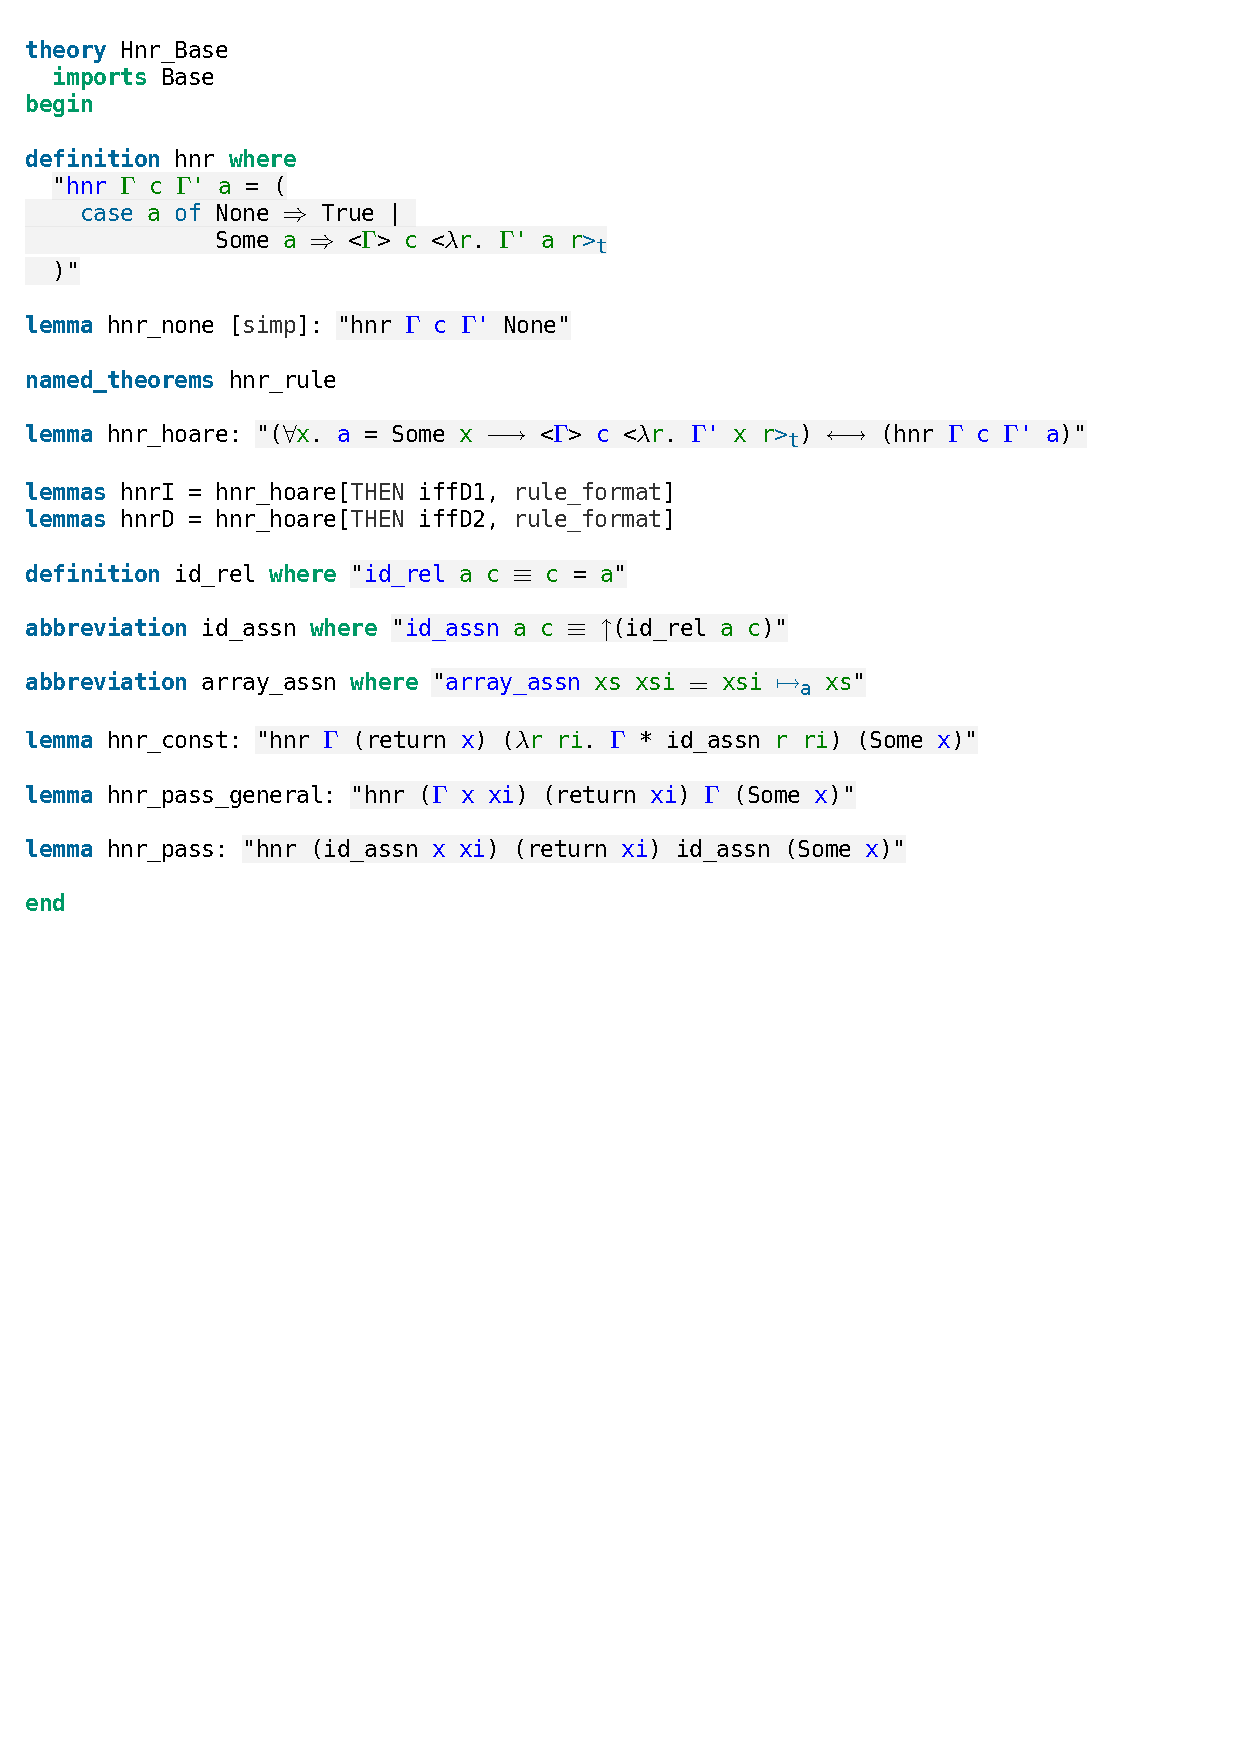
\includegraphics[trim={0 24,8cm 0 2,4cm}, clip, width=1.00\textwidth]{figures/Theory_Hnr_Base.pdf}
    \caption[Hnr predicate]{Hnr predicate}
    \label{fig:hnr_predicate}
\end{figure}

\noindent |a| is defined using an option type, such that the abstract function cannot just be total but also partial. It will help us automate the translation of recursive functions [link].
Consequently, we can directly prove that |hnr| holds for failed or non-terminating functions (\autoref{fig:hnr_none}).

\begin{figure}[htpb]
    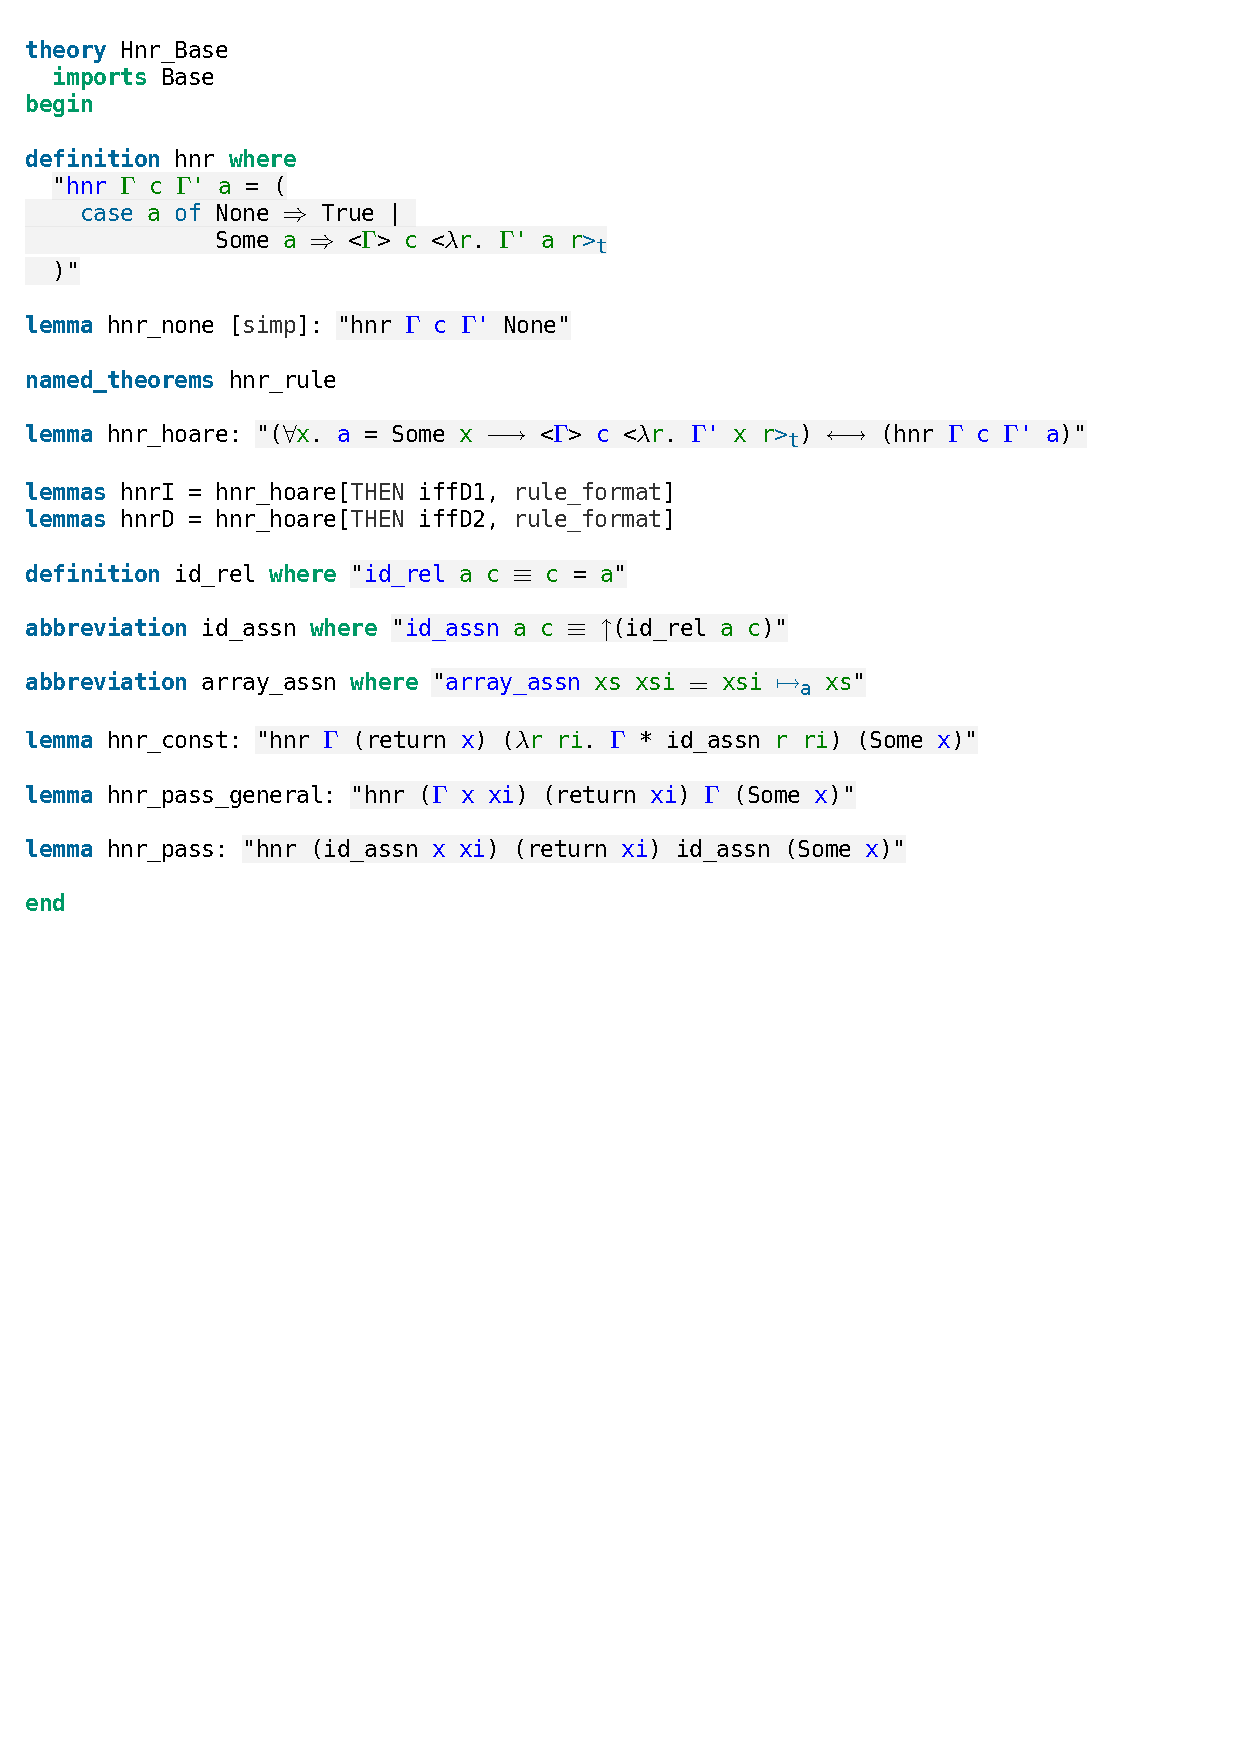
\includegraphics[trim={0 23,8cm 0 5,2cm}, clip, width=1.00\textwidth]{figures/Theory_Hnr_Base.pdf}
    \caption[Failing hnr]{Failing hnr}
    \label{fig:hnr_none}
\end{figure}

\noindent While building up the refinement infrastructure, we assume input functions that have a termination proof and are monadified in the option monad similar to [Wimmer 2018]. That means that every value and constant is assigned to a separate variable using monadic binds or lets. Recursive functions are assumed to be defined using the option monad fix point operator [link]. An automatic translation of functions into the assumed format is not implemented yet [link future work].

\begin{figure}[htpb]
    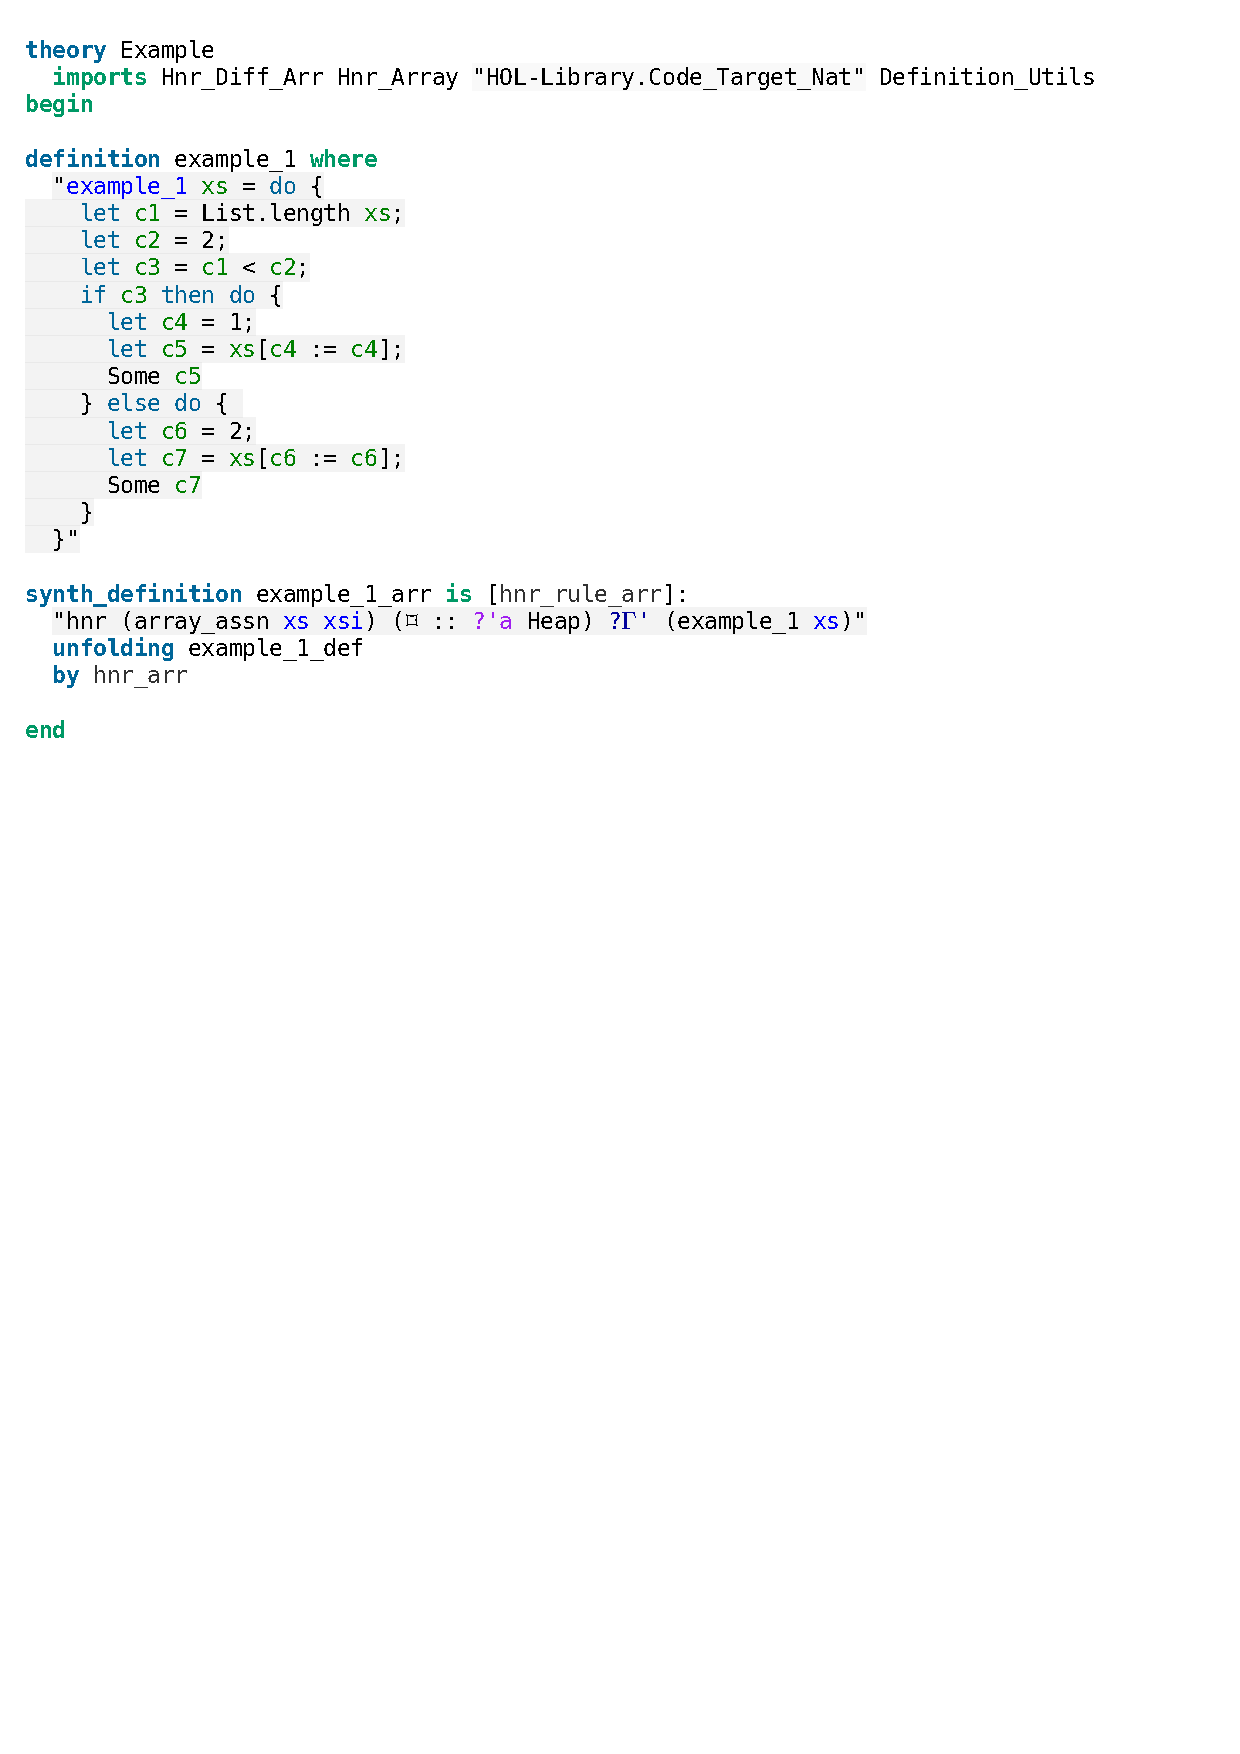
\includegraphics[trim={0 20,2cm 0 2,4cm}, clip, width=1.00\textwidth]{figures/Theory_Example.pdf}
    \caption[Example for a monadified function]{Example for a monadified function}
    \label{fig:monadified_example}
\end{figure}

\noindent We will collect all the |hnr| rules inside a rule set called |hnr|\_|rule| and create conversions between |hnr| and Hoare triples to prove these rules (\autoref{fig:hnr_base}).\\
Further, we will build up the |hnr| rules such that every value has an assertion. The basic assertion therefor is the identity assertion, which states that a value is refined to itself. For that, we wrap the equality operator inside a definition so that no accidental simplifications can happen.

\begin{figure}[htpb]
    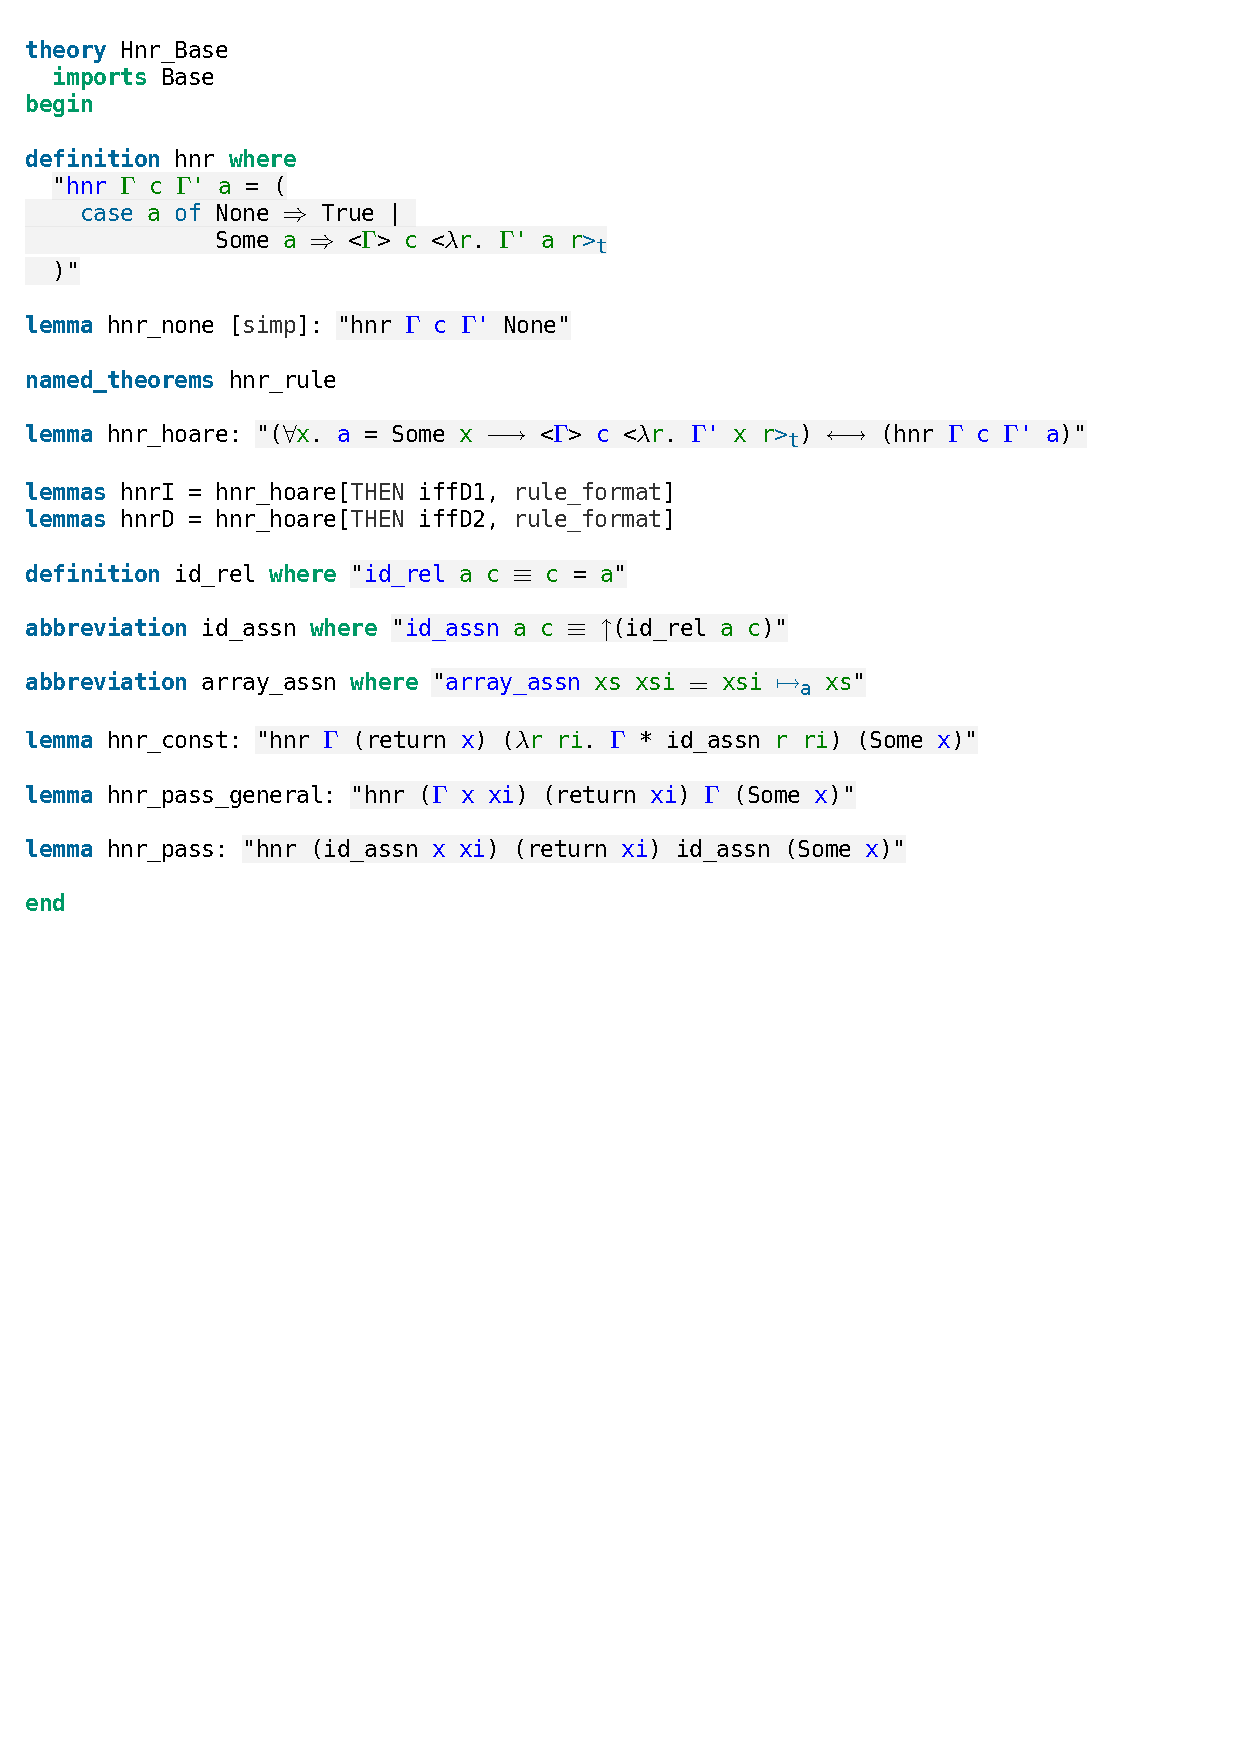
\includegraphics[trim={0 17,8cm 0 6,2cm}, clip, width=1.00\textwidth]{figures/Theory_Hnr_Base.pdf}
    \caption[Basic hnr setup]{Basic hnr setup}
    \label{fig:hnr_base}
\end{figure}

\section{Constant Rule and Pass Rule}\label{section:hnr_const_pass}

To cope with our self-set rule that every value gets an assertion, we introduce a |hnr| rule, which creates identity assertions for constants (\autoref{fig:hnr_const}).

\begin{figure}[htpb]
    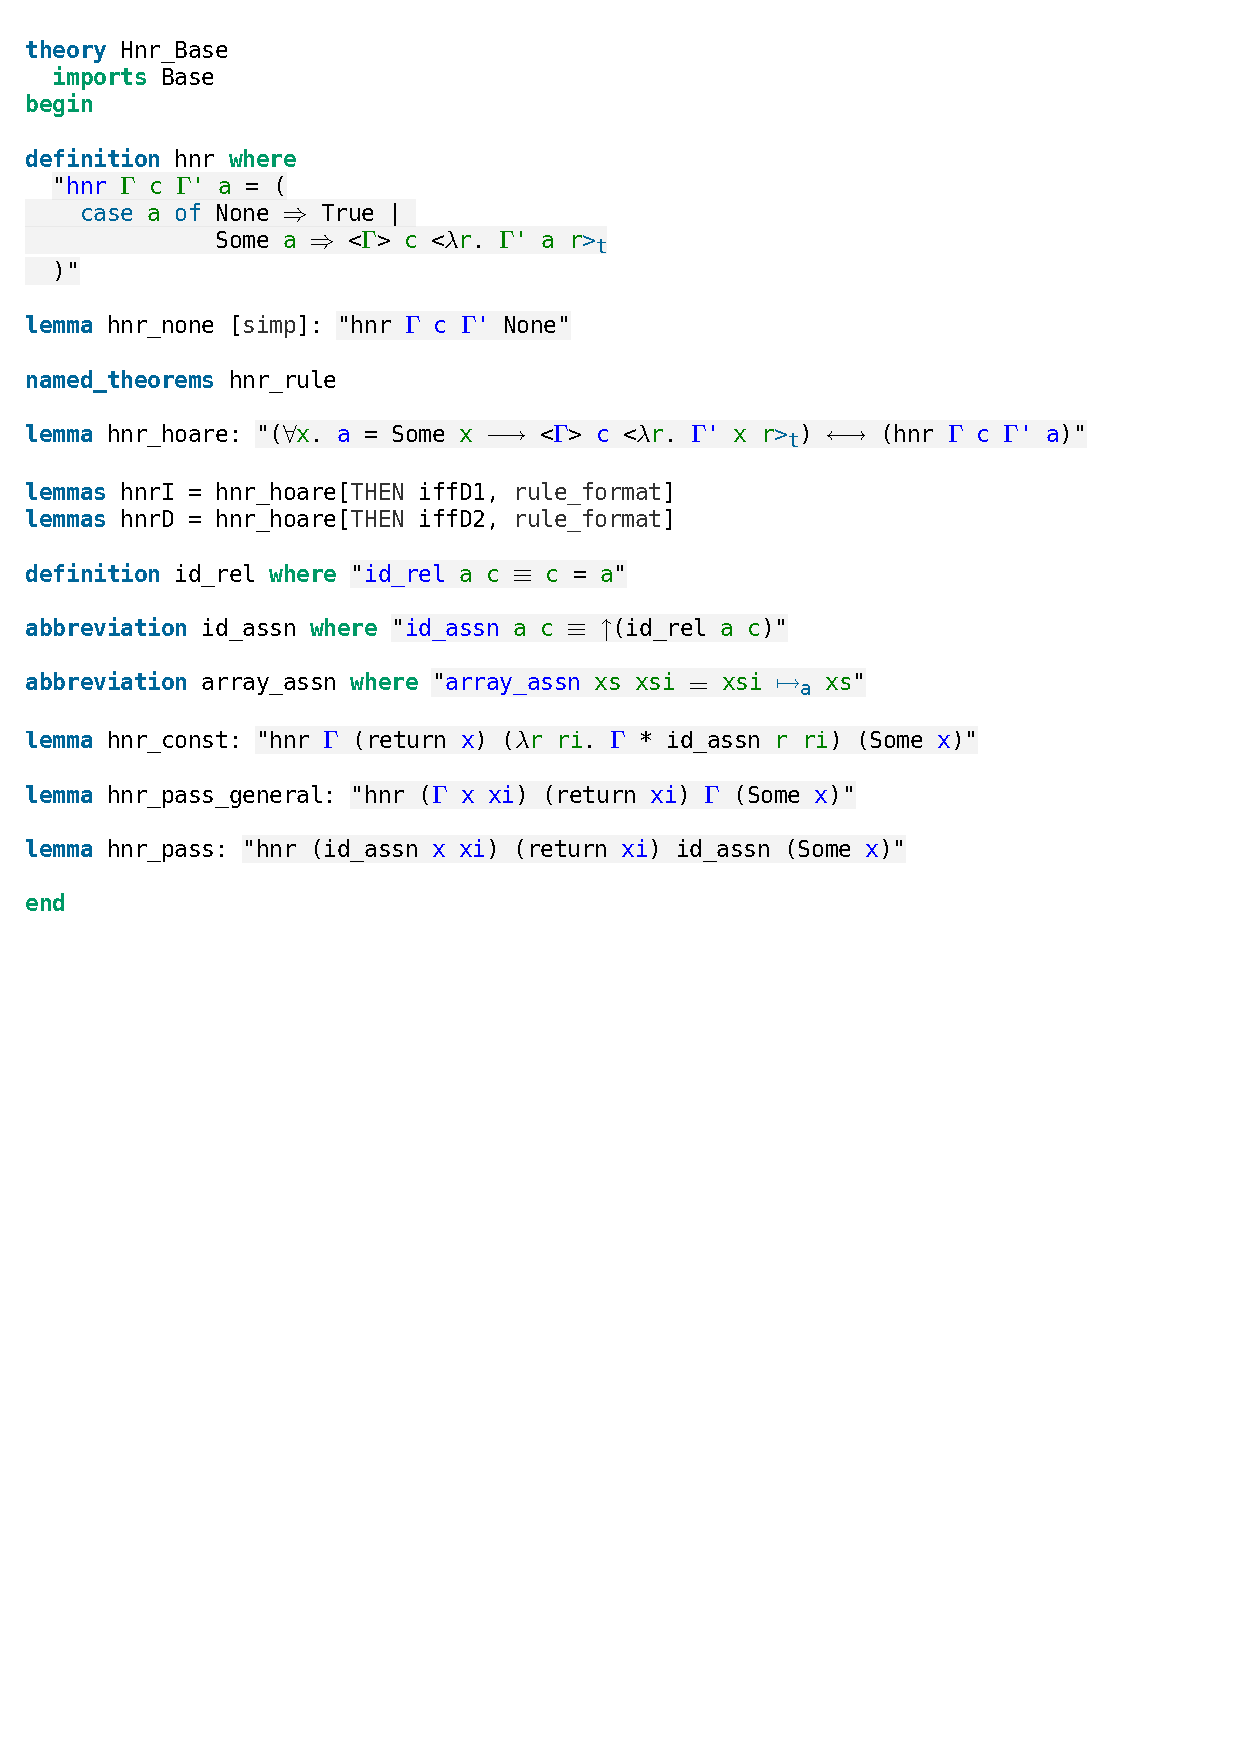
\includegraphics[trim={0 16,8cm 0 12,2cm}, clip, width=1.00\textwidth]{figures/Theory_Hnr_Base.pdf}
    \caption[Constant rule]{Constant rule}
    \label{fig:hnr_const}
\end{figure}

\noindent If no other |hnr| rule can be applied, this will be our fallback rule. The proof for the rule is a conversion of the |hnr| predicate to a Hoare triple, and then the separation logic proof automation does the rest.
In the case that we already have an assertion for a value, we do not need to create a new assertion but can simply pass on the existing one. \autoref{fig:hnr_pass} shows a general rule for that purpose. Later, we will specify this rule for the different assertion types, for example, the diff array master assertion. However, in the first step, we just specify it for identity assertions.

\begin{figure}[htpb]
    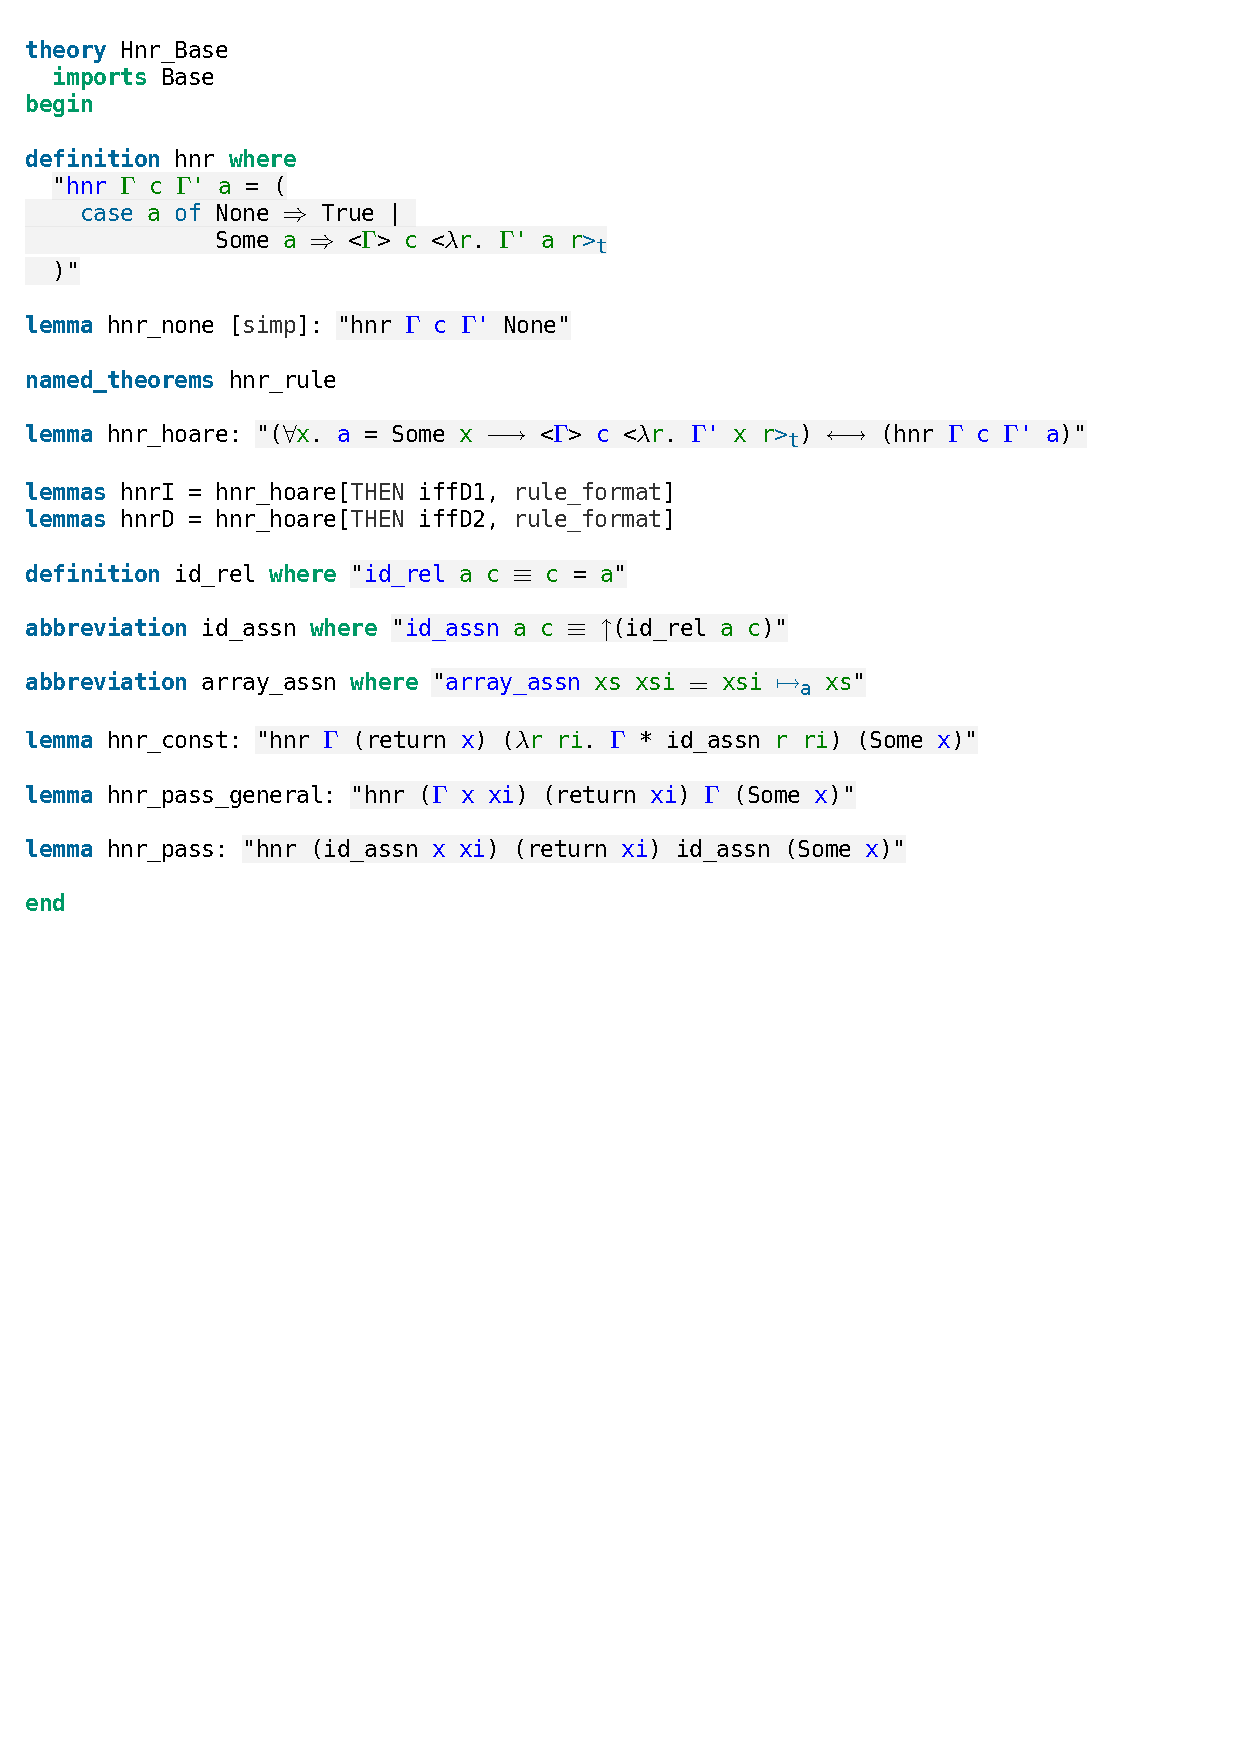
\includegraphics[trim={0 15cm 0 13,2cm}, clip, width=1.00\textwidth]{figures/Theory_Hnr_Base.pdf}
    \caption[Pass rule]{Pass rule}
    \label{fig:hnr_pass}
\end{figure}

\noindent Again, the proof is a conversion to a Hoare triple and then separation logic proof automation.

\section{Keep - Drop}\label{section:keep_drop}

Since Imperative/HOL translates by default to a garbage-collected language, we need a facility to drop assertions of data structures that go out of scope. In the branches of the |if|-statement in \autoref{fig:monadified_example}, for example, the variables |c4| - |c7| are going out of scope after the branches are left, such that it would not be possible to keep assertions for them. 
We create the definition in \autoref{fig:keep_drop} to separate the assertions we want to keep and drop in our |hnr| rules.

\begin{figure}[htpb]
    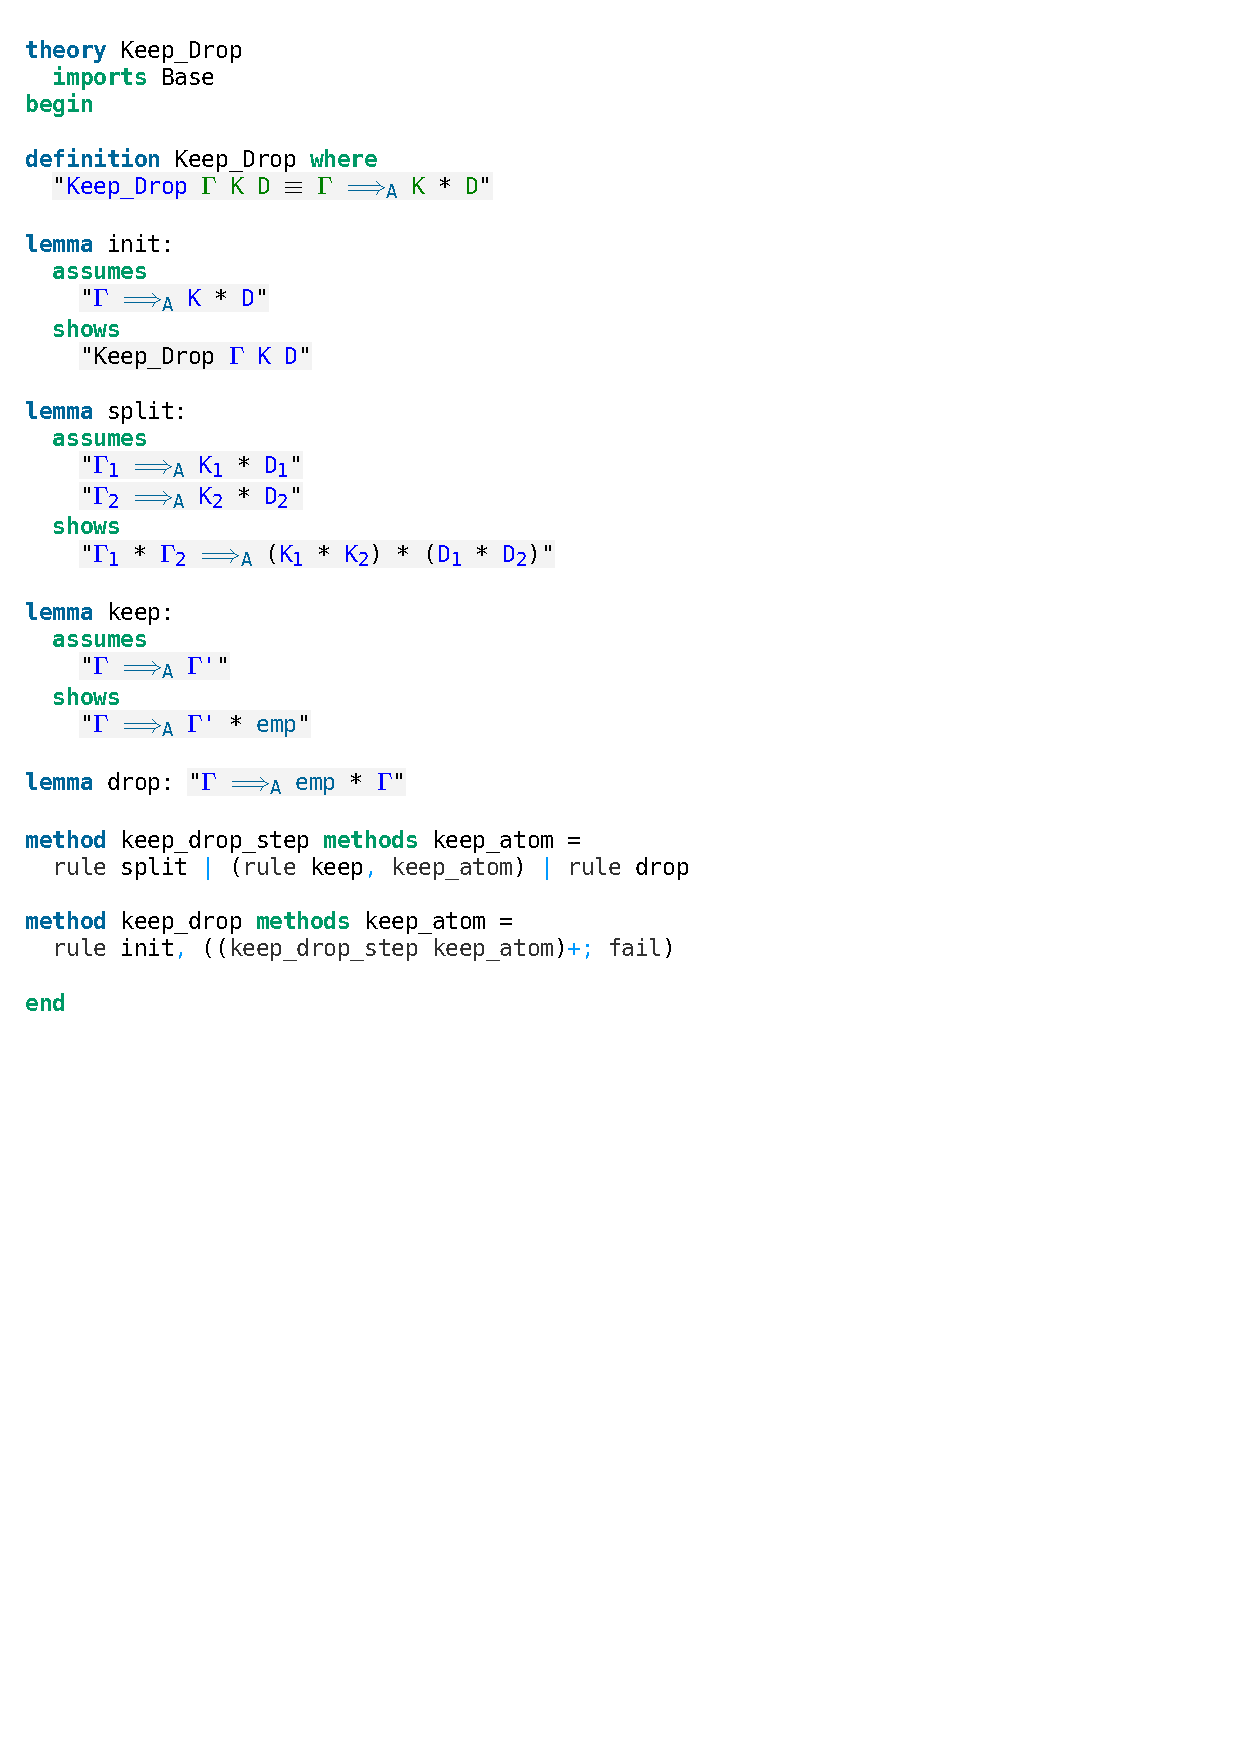
\includegraphics[trim={0 26,2cm 0 2,4cm}, clip, width=1.00\textwidth]{figures/Theory_Keep_Drop.pdf}
    \caption[Separation of assertions to keep or drop]{Separation of assertions to keep or drop}
    \label{fig:keep_drop}
\end{figure}

\noindent $\Gamma$ describes all our current assertions, which we then split into what we want to keep (|K|) and what we want to drop (|D|). For instance, rules for translating case distinctions will produce such goals. To resolve them, we first unfold the definition by using the initialization rule (\autoref{fig:keep_drop_init}).

\begin{figure}[htpb]
    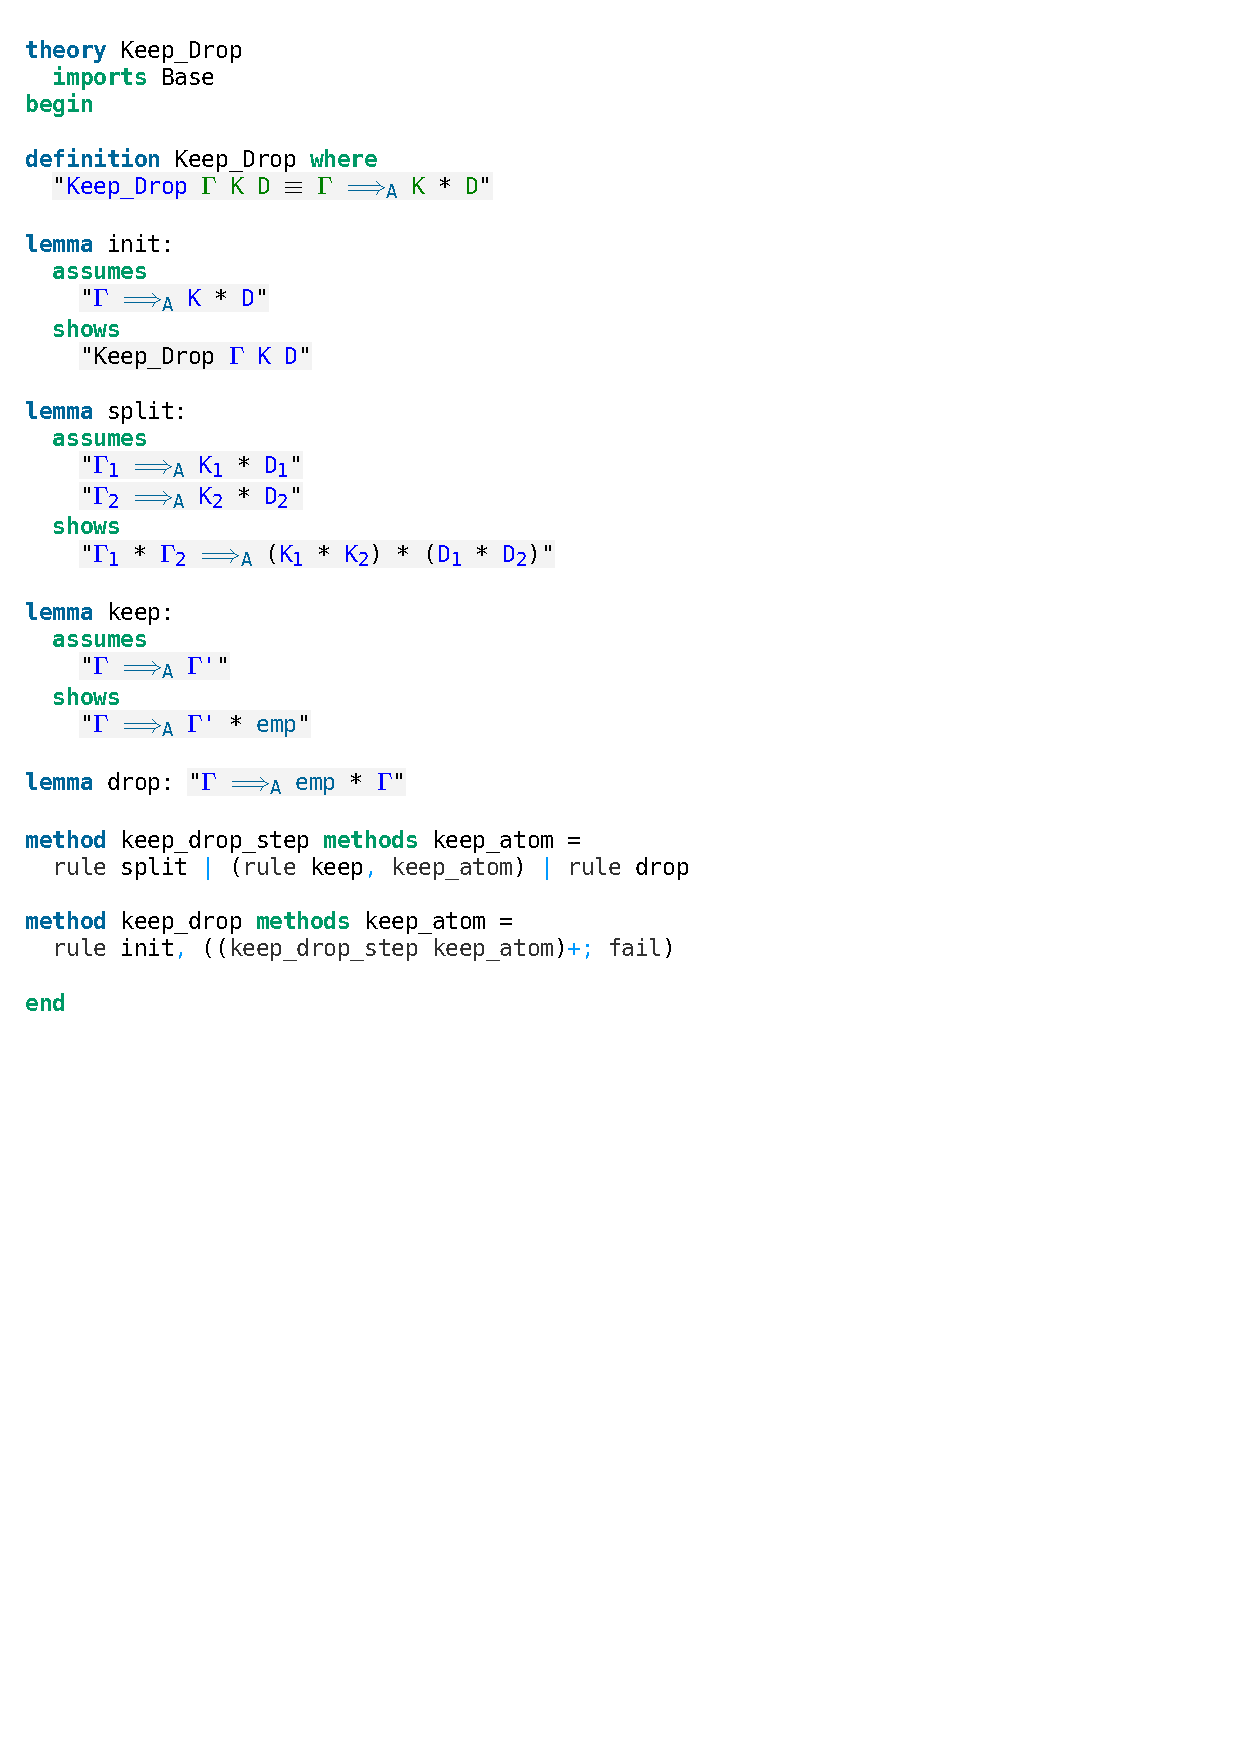
\includegraphics[trim={0 23,4cm 0 3,8cm}, clip, width=1.00\textwidth]{figures/Theory_Keep_Drop.pdf}
    \caption[Keep-Drop initialization rule]{Keep - Drop initialization rule}
    \label{fig:keep_drop_init}
\end{figure}

\noindent After that, there are three different rules (\autoref{fig:keep_drop_rules}) that we try to apply to resolve the goal:\\
1. We try to split up the assertion as far as possible using the separation conjunction.\\
2. If we cannot split up the assertion anymore, we try to keep it by replacing its drop part with the empty assertion. Note that we do not use $\Gamma$ $\Longrightarrow_A$ |emp *| $\Gamma'$ here to allow more sophisticated matching methods than simple entailment. For example, for matching master assertions, we want to allow different orders of elements inside it.\\
3. If keeping an assertion does not work, we drop it by replacing its keep part with the empty assertion and putting the whole assertion into the drop part.\\
We can use an Eisbach method (\autoref{fig:keep_drop_methods}) to put these three rules together as described. Further, we put the initialization rule in front of it and execute the step as often as possible to resolve keep-drop statements automatically.

\begin{figure}[htpb]
    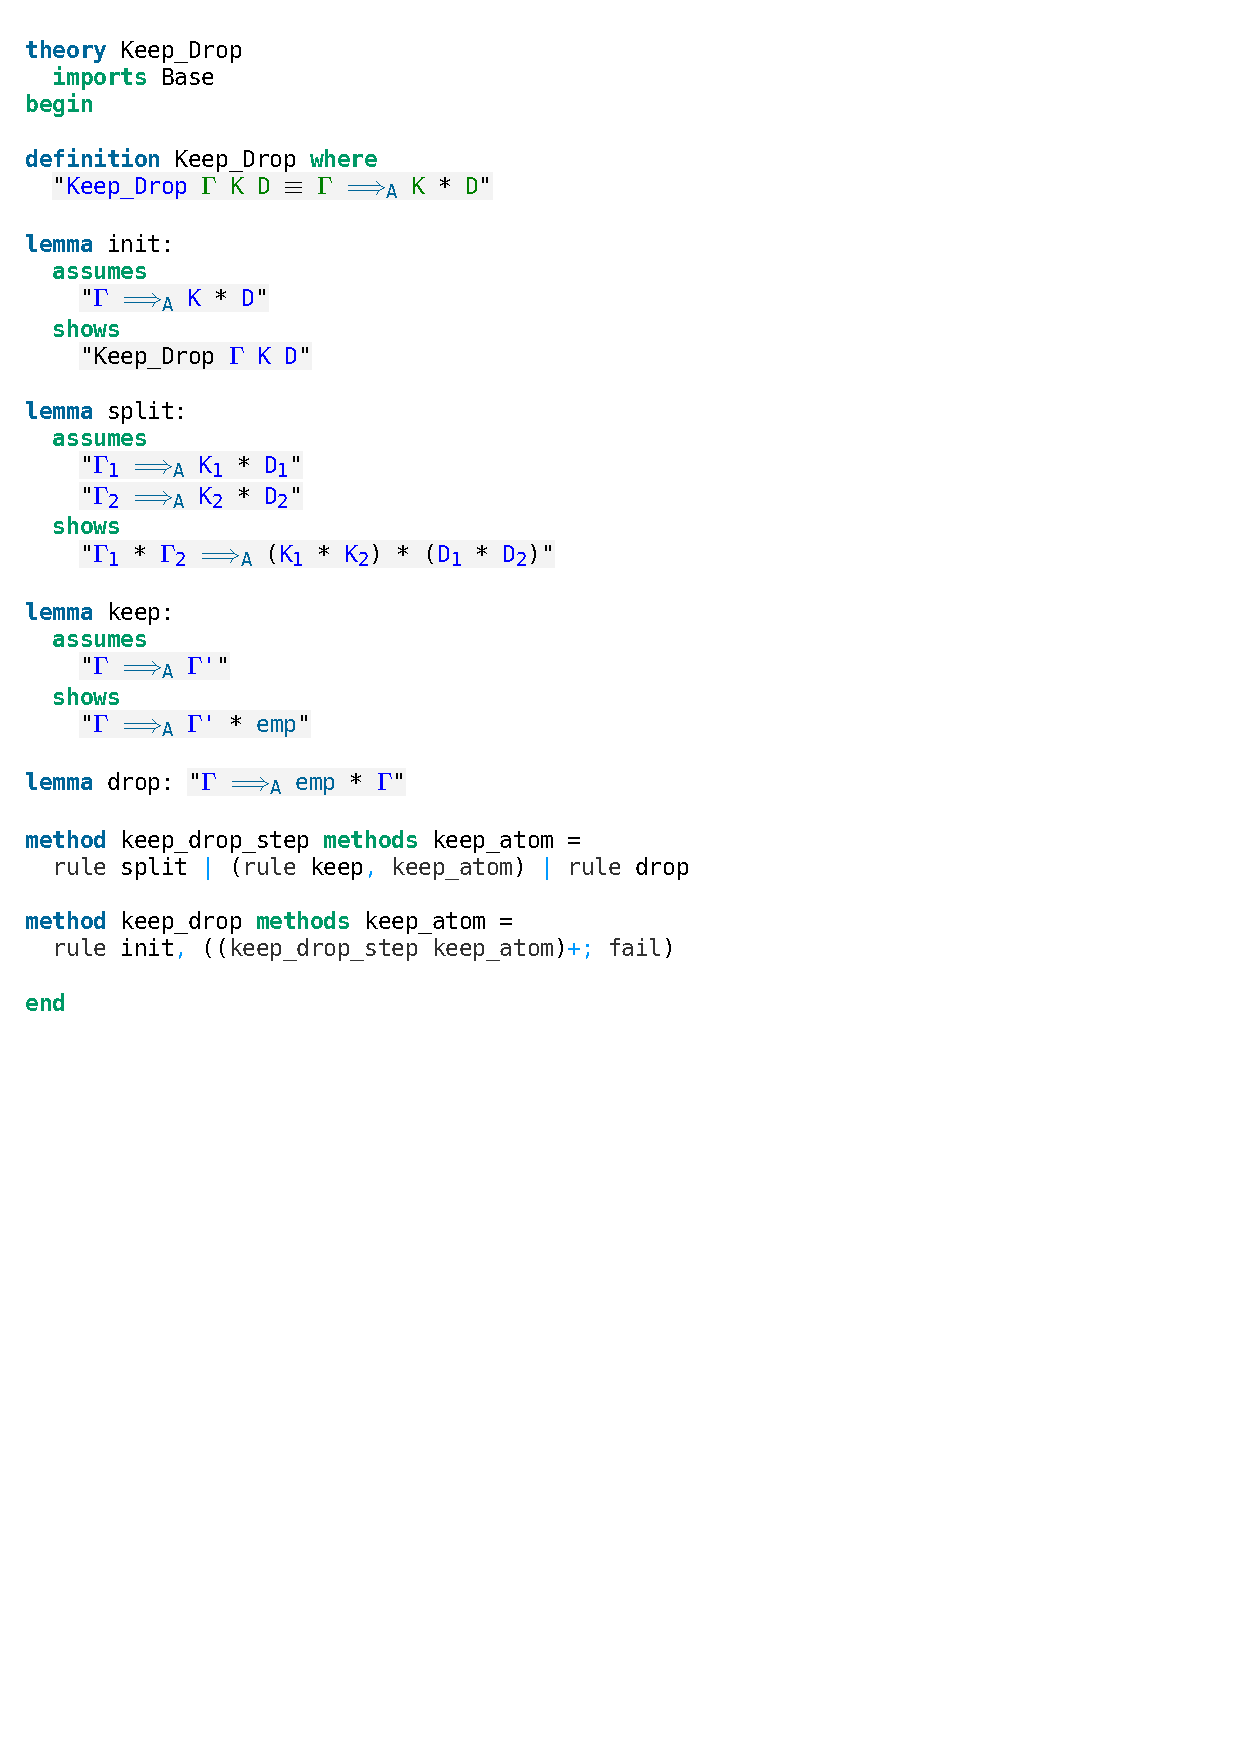
\includegraphics[trim={0 16,2cm 0 6,8cm}, clip, width=1.00\textwidth]{figures/Theory_Keep_Drop.pdf}
    \caption[Keep-Drop rules]{Keep - Drop rules}
    \label{fig:keep_drop_rules}
\end{figure}

\begin{figure}[htpb]
    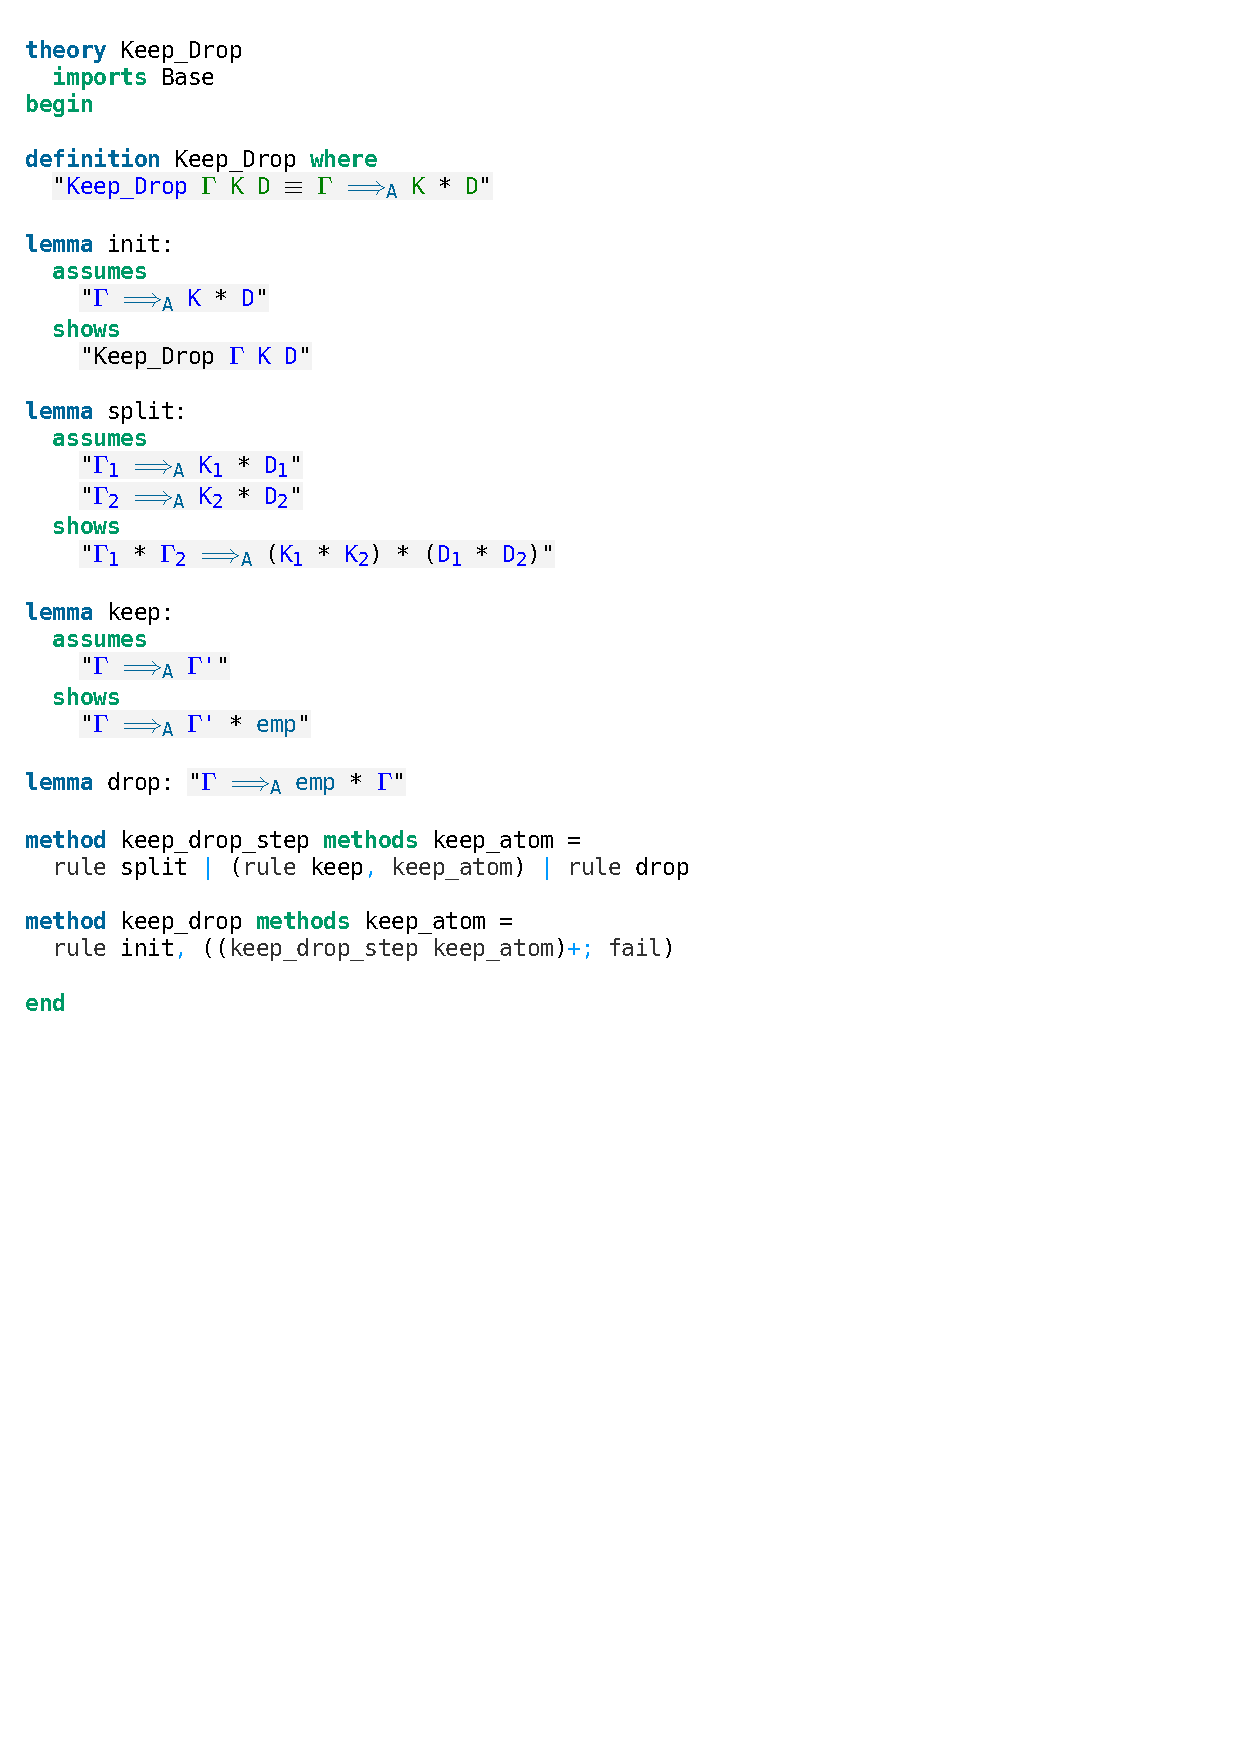
\includegraphics[trim={0 13,4cm 0 14cm}, clip, width=1.00\textwidth]{figures/Theory_Keep_Drop.pdf}
    \caption[Keep-Drop methods]{Keep - Drop methods}
    \label{fig:keep_drop_methods}
\end{figure}

\section{Normalization}

For example, after resolving a keep-drop clause, the assertions might not be normalized anymore, meaning that the assertion can contain empty clauses and does not have the default bracketing. We introduce the definition in \autoref{fig:norm} to mark places where this can happen.

\begin{figure}[htpb]
    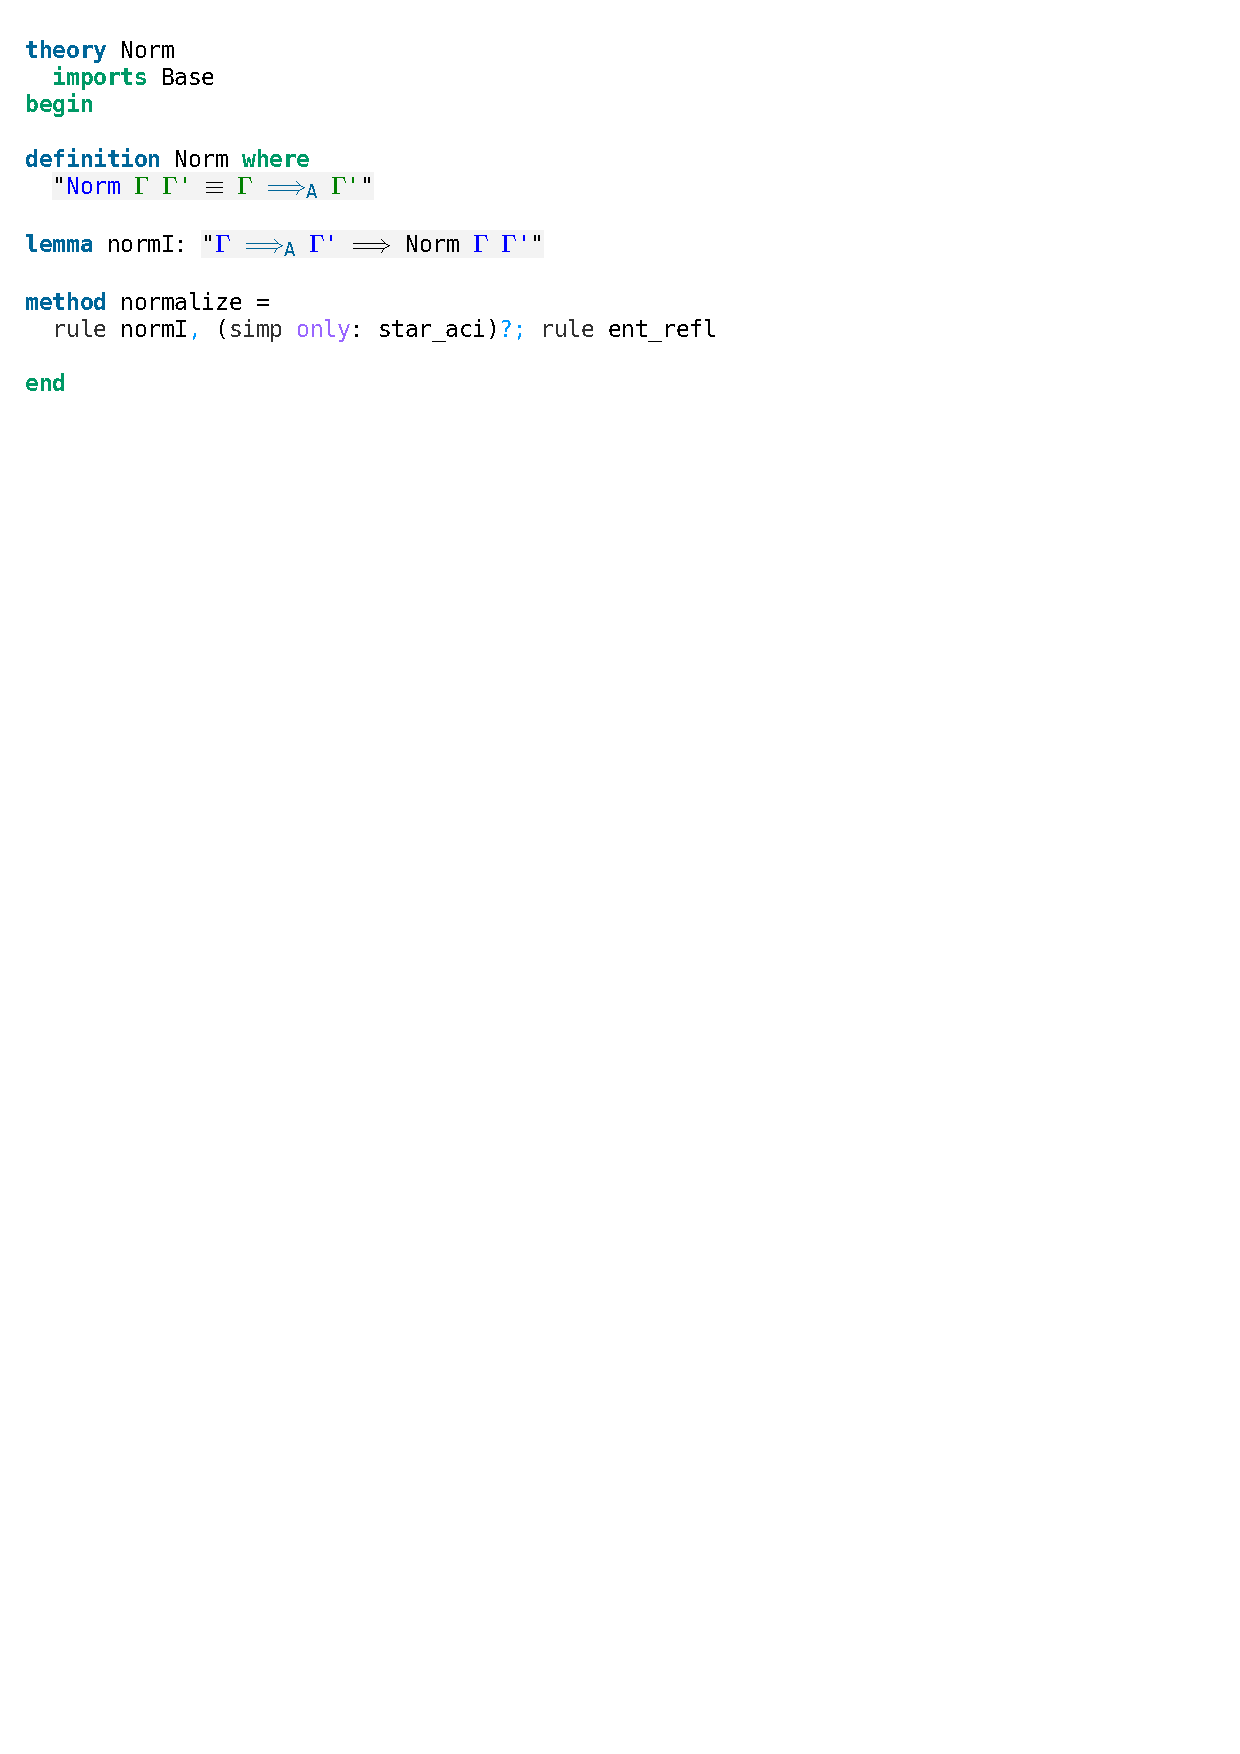
\includegraphics[trim={0 26,2cm 0 2,4cm}, clip, width=1.00\textwidth]{figures/Theory_Norm.pdf}
    \caption[Normalization definition]{Normalization definition}
    \label{fig:norm}
\end{figure}

\noindent When reaching such a goal, we can do the normalization by first unfolding the definition. The separation logic library has a rule collection called |star|\_|aci|, which can then normalize the assertion by giving it to the simplifier. After that, as the last step, we can solve the entailment by reflexivity. 

\begin{figure}[htpb]
    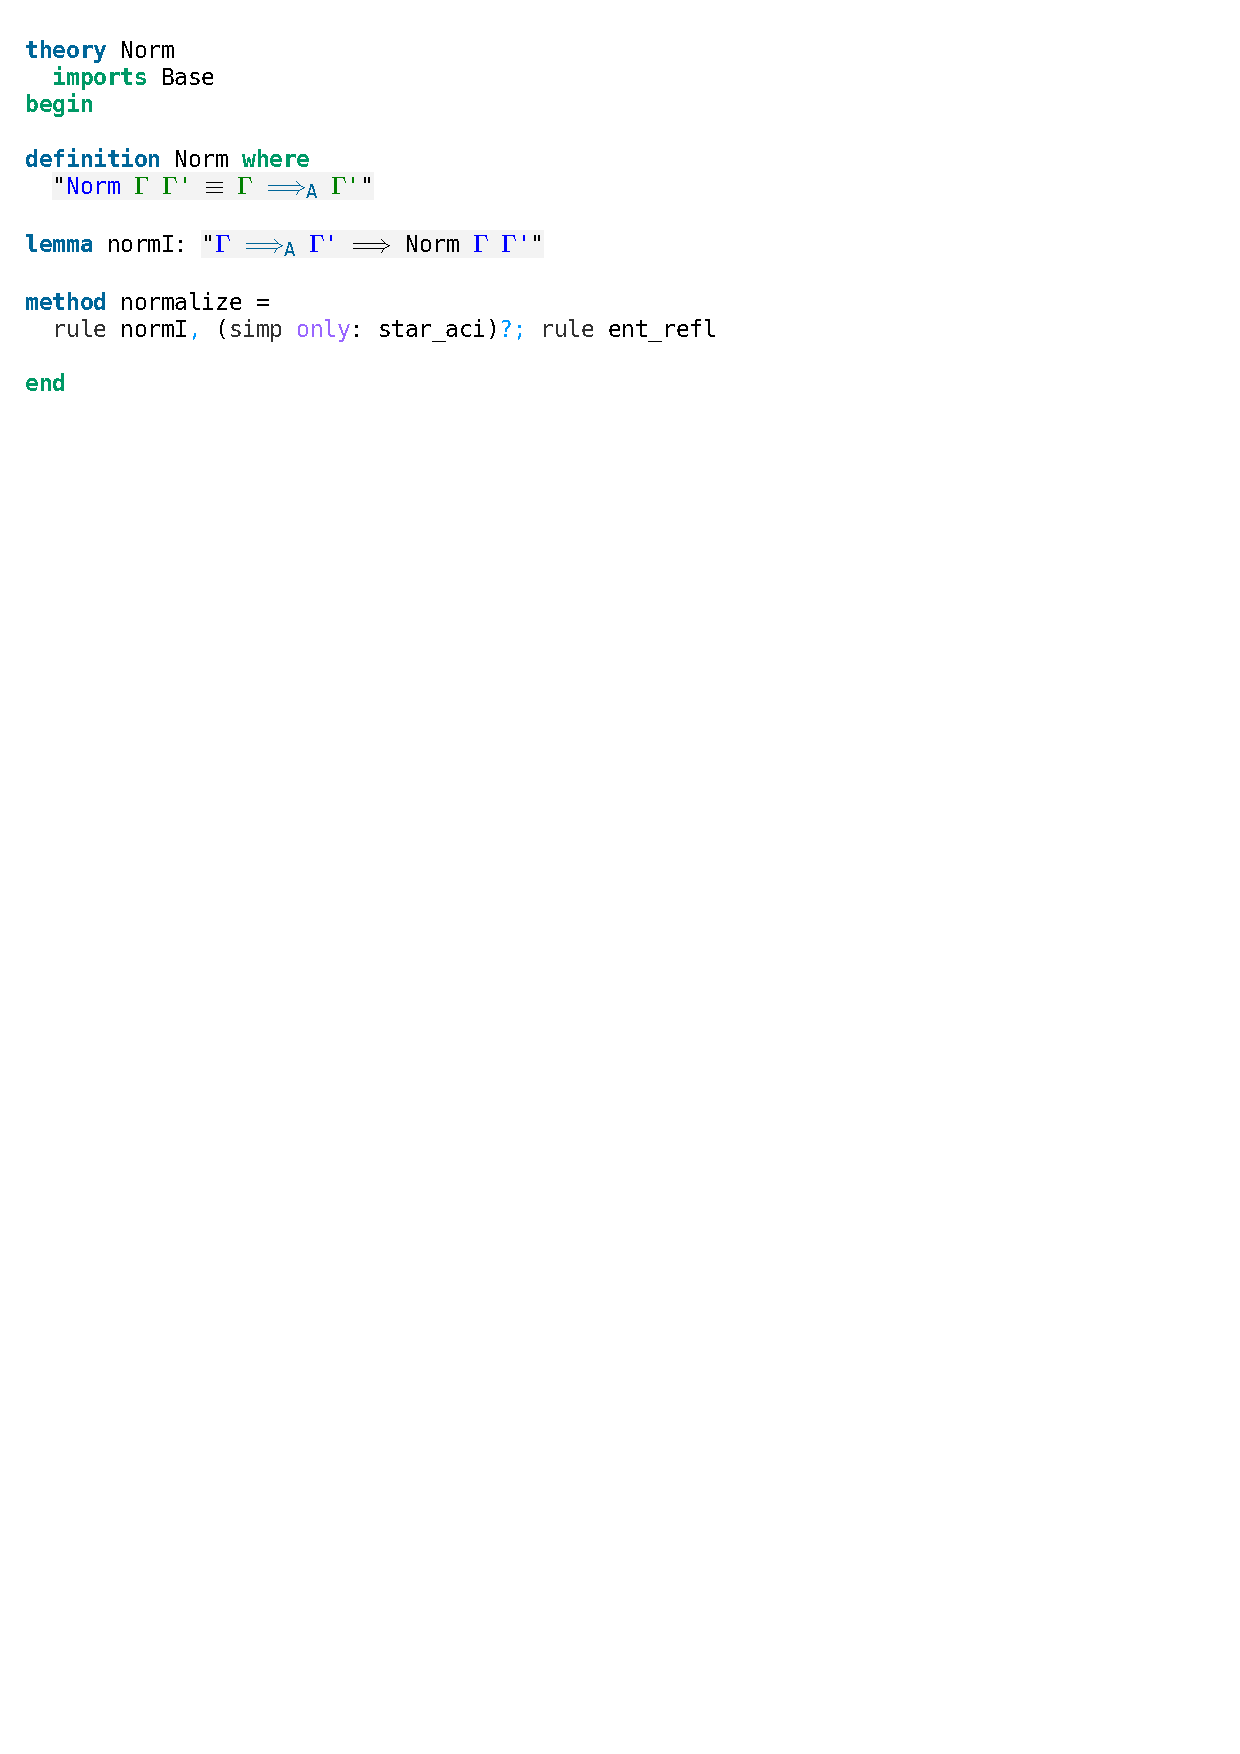
\includegraphics[trim={0 23,9cm 0 3,9cm}, clip, width=1.00\textwidth]{figures/Theory_Norm.pdf}
    \caption[Normalization procedure]{Normalization procedure}
    \label{fig:norm_procedure}
\end{figure}

\section{Merge}

After an |if|- or |case|-statement, every branch has its own assertion, which we need to merge into one to continue with the function refinement. As for keep-drop and normalization before, we introduce a definition again (\autoref{fig:merge}).

\begin{figure}[htpb]
    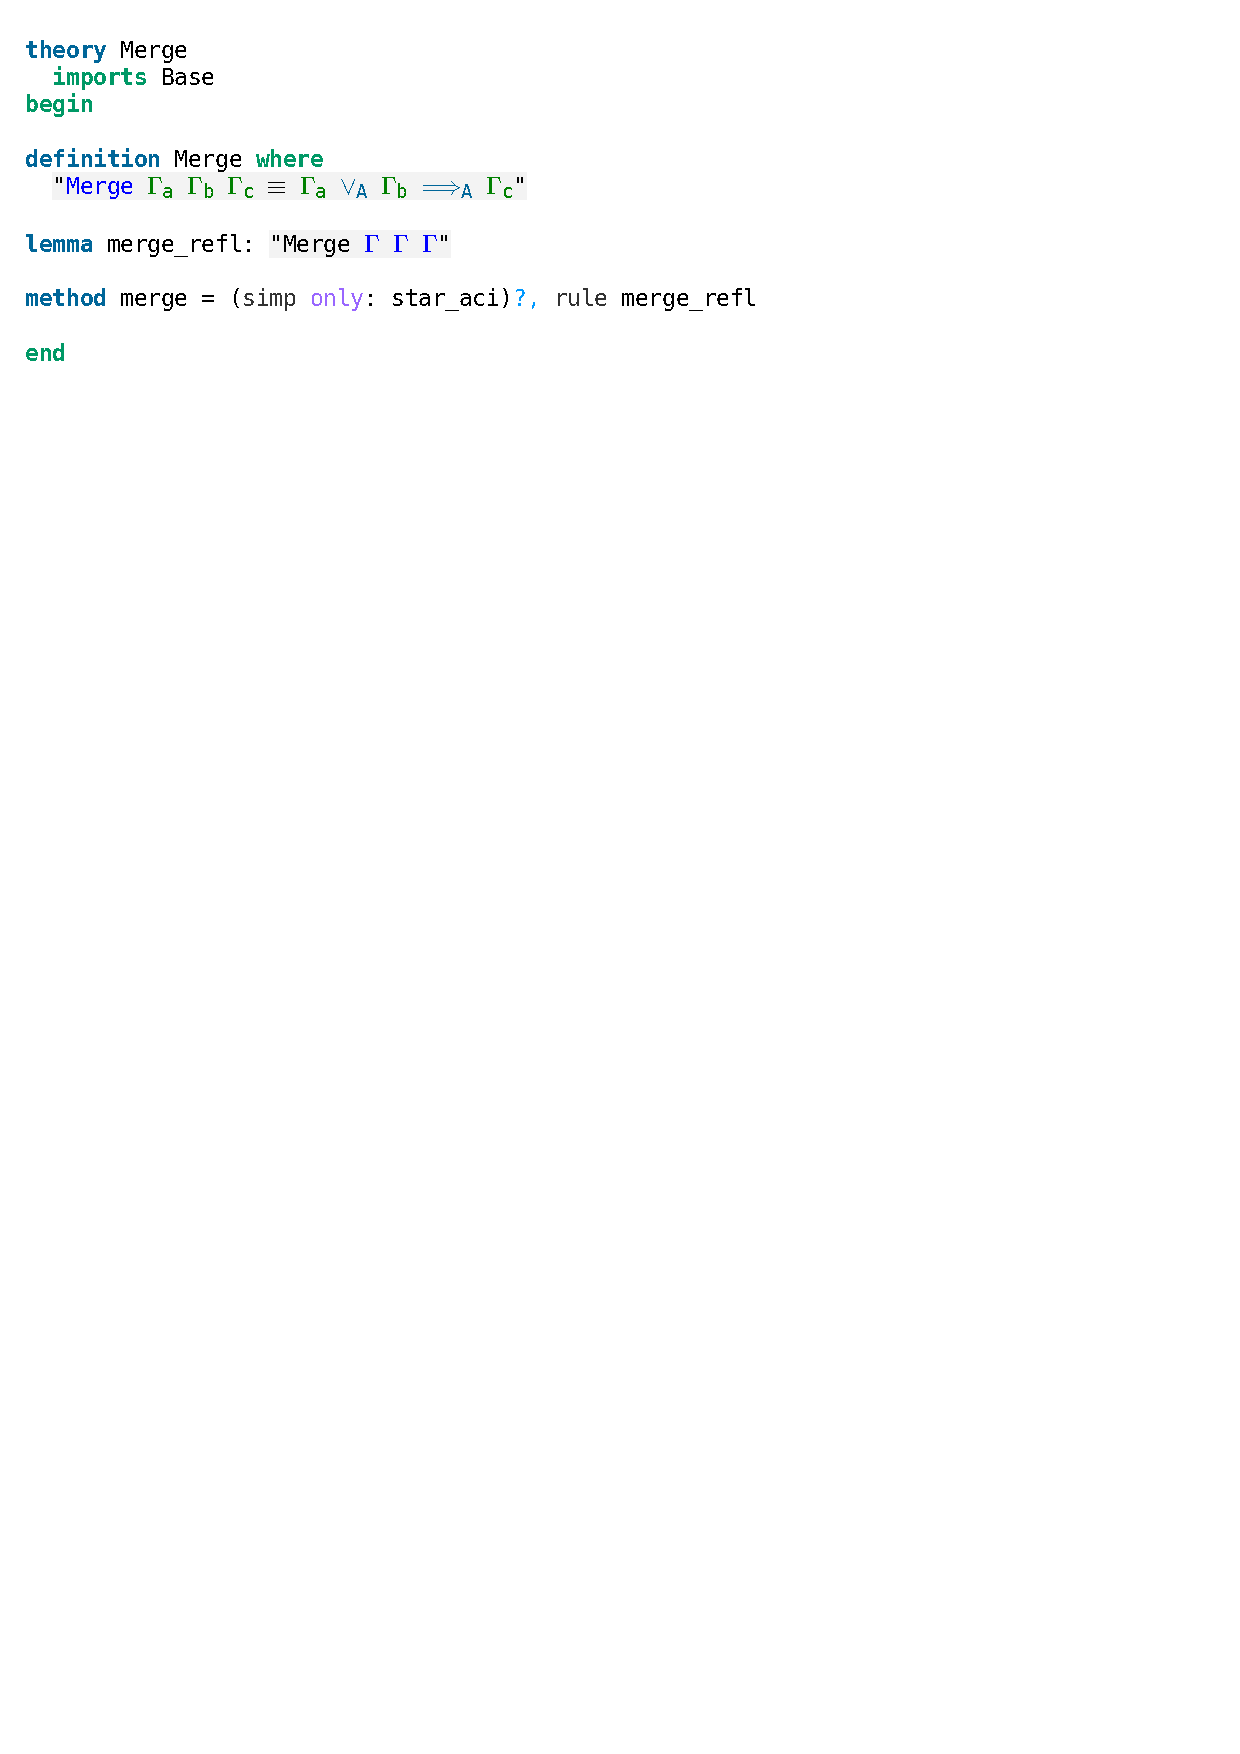
\includegraphics[trim={0 26,2cm 0 2,4cm}, clip, width=1.00\textwidth]{figures/Theory_Merge.pdf}
    \caption[Merge definition]{Merge definition}
    \label{fig:merge}
\end{figure}

\noindent The first two parameters, $\Gamma_a$ and $\Gamma_b$ describe the postconditions of two different branches. We connect them with a separation logic disjunction because either one or the other branch runs. The common elements of the two assertions then come together in $\Gamma_c$.
Because of our keep drop routine, which we expect to be executed prior to the merge, we can assume that the postconditions of both branches are the same. Since they may not be normalized, we normalize them in the same way as in the previous section and then resolve the merge by reflexivity. In \autoref{fig:merge_method} we put these steps together using an Eisbach method.

\begin{figure}[htpb]
    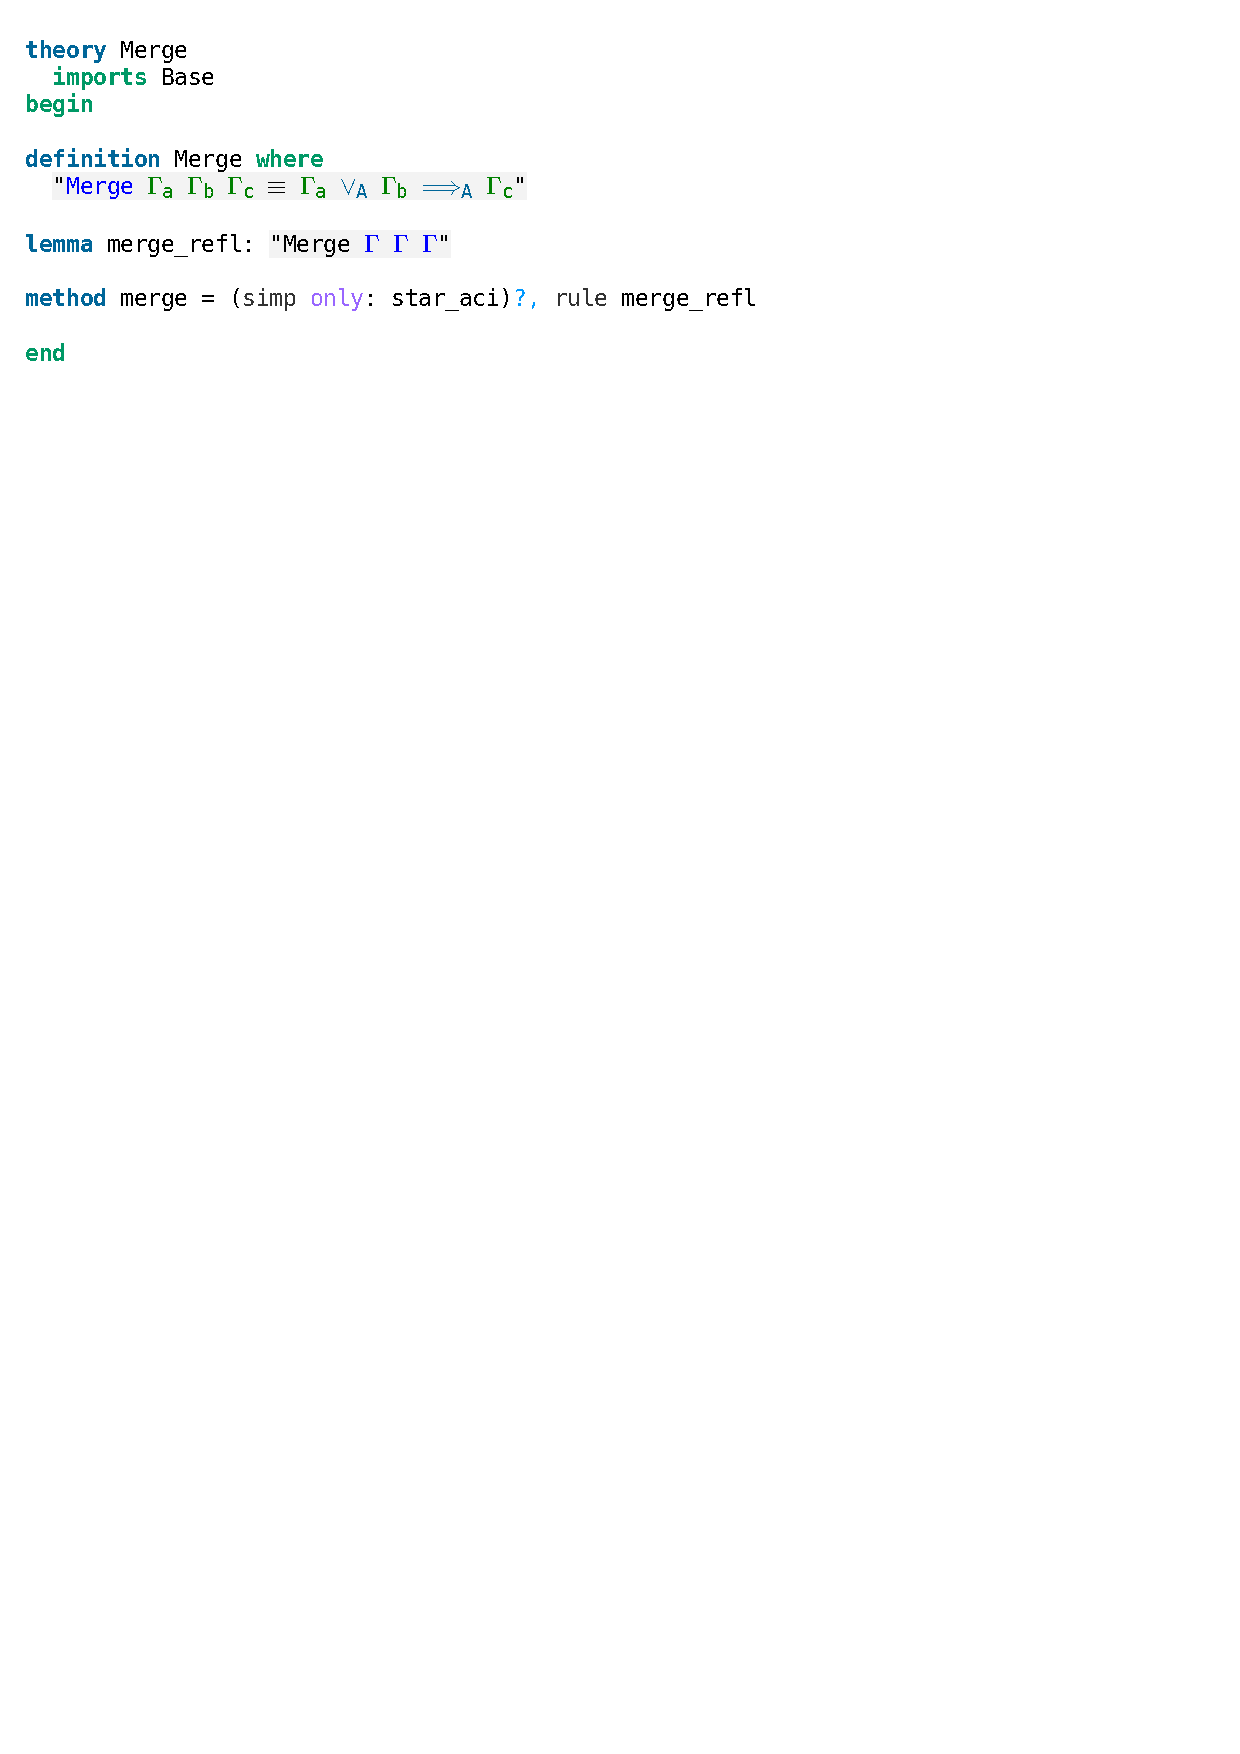
\includegraphics[trim={0 24,4cm 0 3,9cm}, clip, width=1.00\textwidth]{figures/Theory_Merge.pdf}
    \caption[Merge method]{Merge method}
    \label{fig:merge_method}
\end{figure}

\section{Hnr Rules}

In the following, we define some general |hnr| conversion rules of language statements, which we collect in the previously defined rule set called |hnr|\_|rule| (\autoref{fig:hnr_base}).

\subsection{Tuple}

When reaching the creation of a tuple, we can translate it into the binding of two already translated programs, which we then combine into a tuple. As a result, we have two |hnr| clauses in the assumption. The first of these has the same precondition as the conclusion. The second takes the postcondition of the first as its precondition since they run one after the other, and the second can depend on the result of the first one. The postcondition of the second clause is then consequently the postcondition of the conclusion, which can depend on the results of both clauses. To satisfy these dependencies in the conclusion, we deconstruct the tuple using the selectors for its first and second elements. \\
The proof of this rule is a conversion of the |hnr|s to Hoare triples and separation logic proof automation.

\begin{figure}[htpb]
    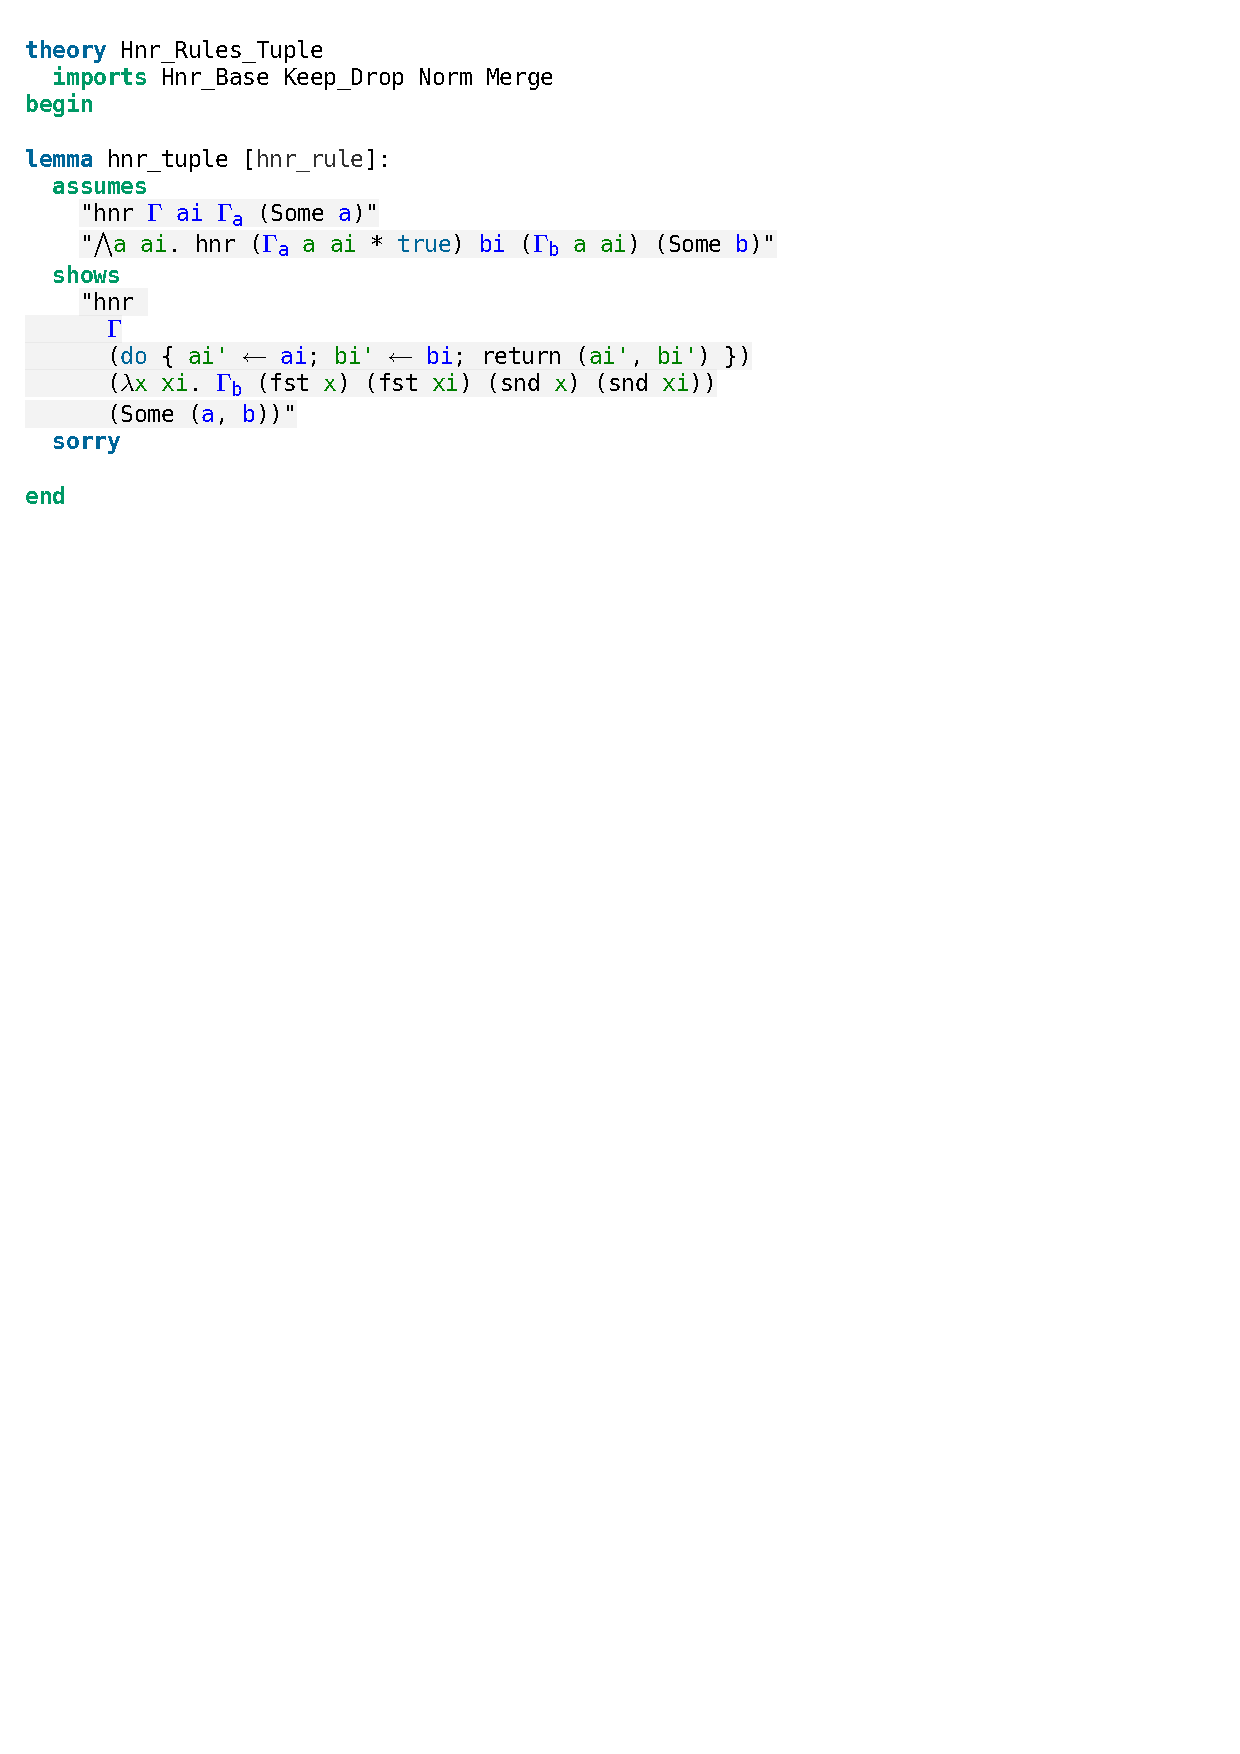
\includegraphics[trim={0 22,4cm 0 2,4cm}, clip, width=1.00\textwidth]{figures/Theory_Hnr_Rules_Tuple.pdf}
    \caption[Hnr tuple rule]{Hnr tuple rule}
    \label{fig:hnr_tuple}
\end{figure}

\subsection{Bind}

When binding a variable in the option monad (equivalent to let-bindings), we naturally also want to have a bind in the heap monad. Therefore, we create two |hnr| clauses as assumptions to achieve that - one for the bound value and one for the context of the bound value. Additionally, we introduce a keep-drop clause to drop the dependencies on the locally bound variable again. As described in \autoref{section:keep_drop}, we always need a normalization clause accompanying the keep-drop clause.\\
The proof of the rule works by converting to Hoare triples again, then using the proof automation, and unfolding and applying the keep-drop and normalization definitions.

\begin{figure}[htpb]
    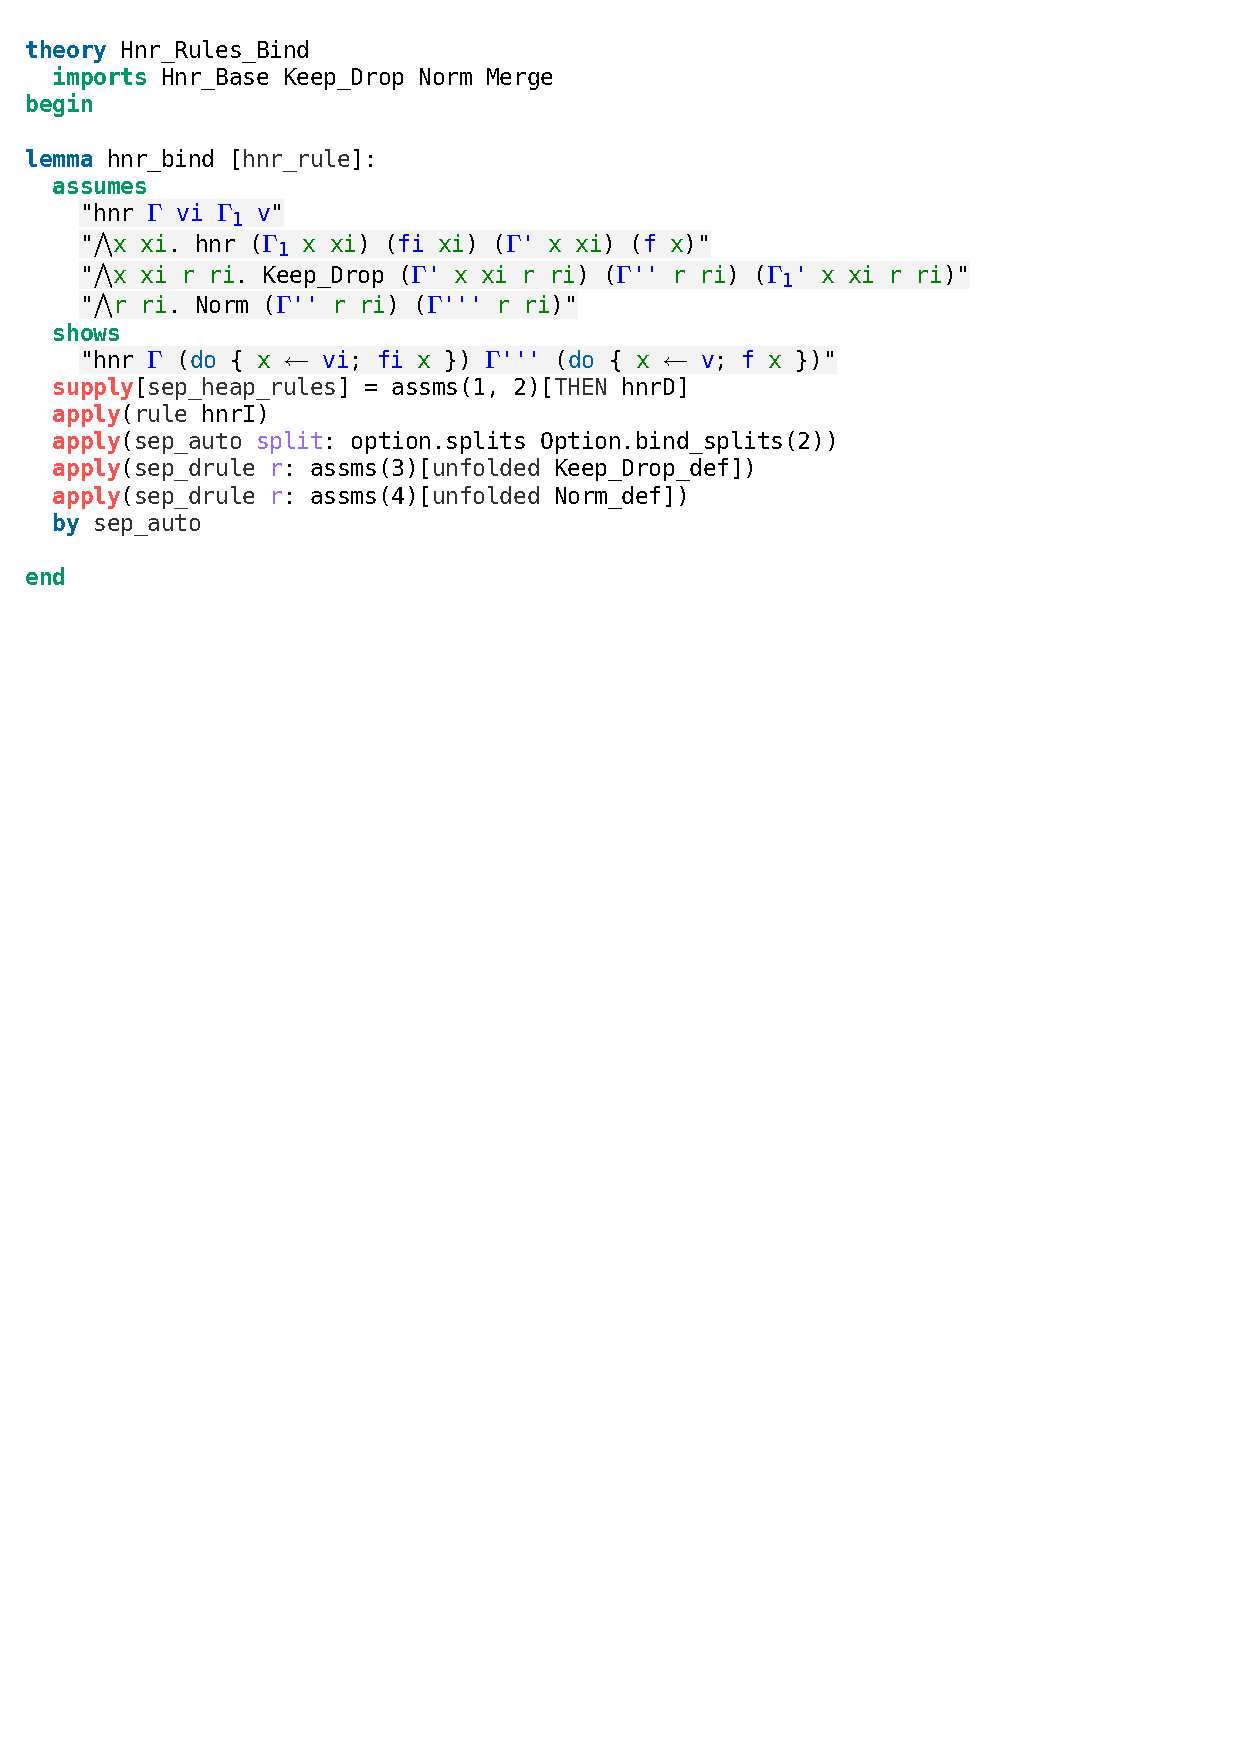
\includegraphics[trim={0 23,4cm 0 2,4cm}, clip, width=1.00\textwidth]{figures/Theory_Hnr_Rules_Bind.pdf}
    \caption[Hnr bind rule]{Hnr bind rule}
    \label{fig:hnr_bind}
\end{figure}

\subsection{If}

To convert an |if|-statement, we assume that we have already converted its two branches and have an identity assertion for its condition and the condition's abstraction. Additionally, we need a merge clause, which merges the two postconditions of the branches to the postcondition of the whole statement.\\
The proof of the rule consists of unfolding the merge definition, destructuring the |if|-statement, and using rules for disjunctions in separation logic assertions.

\begin{figure}[htpb]
    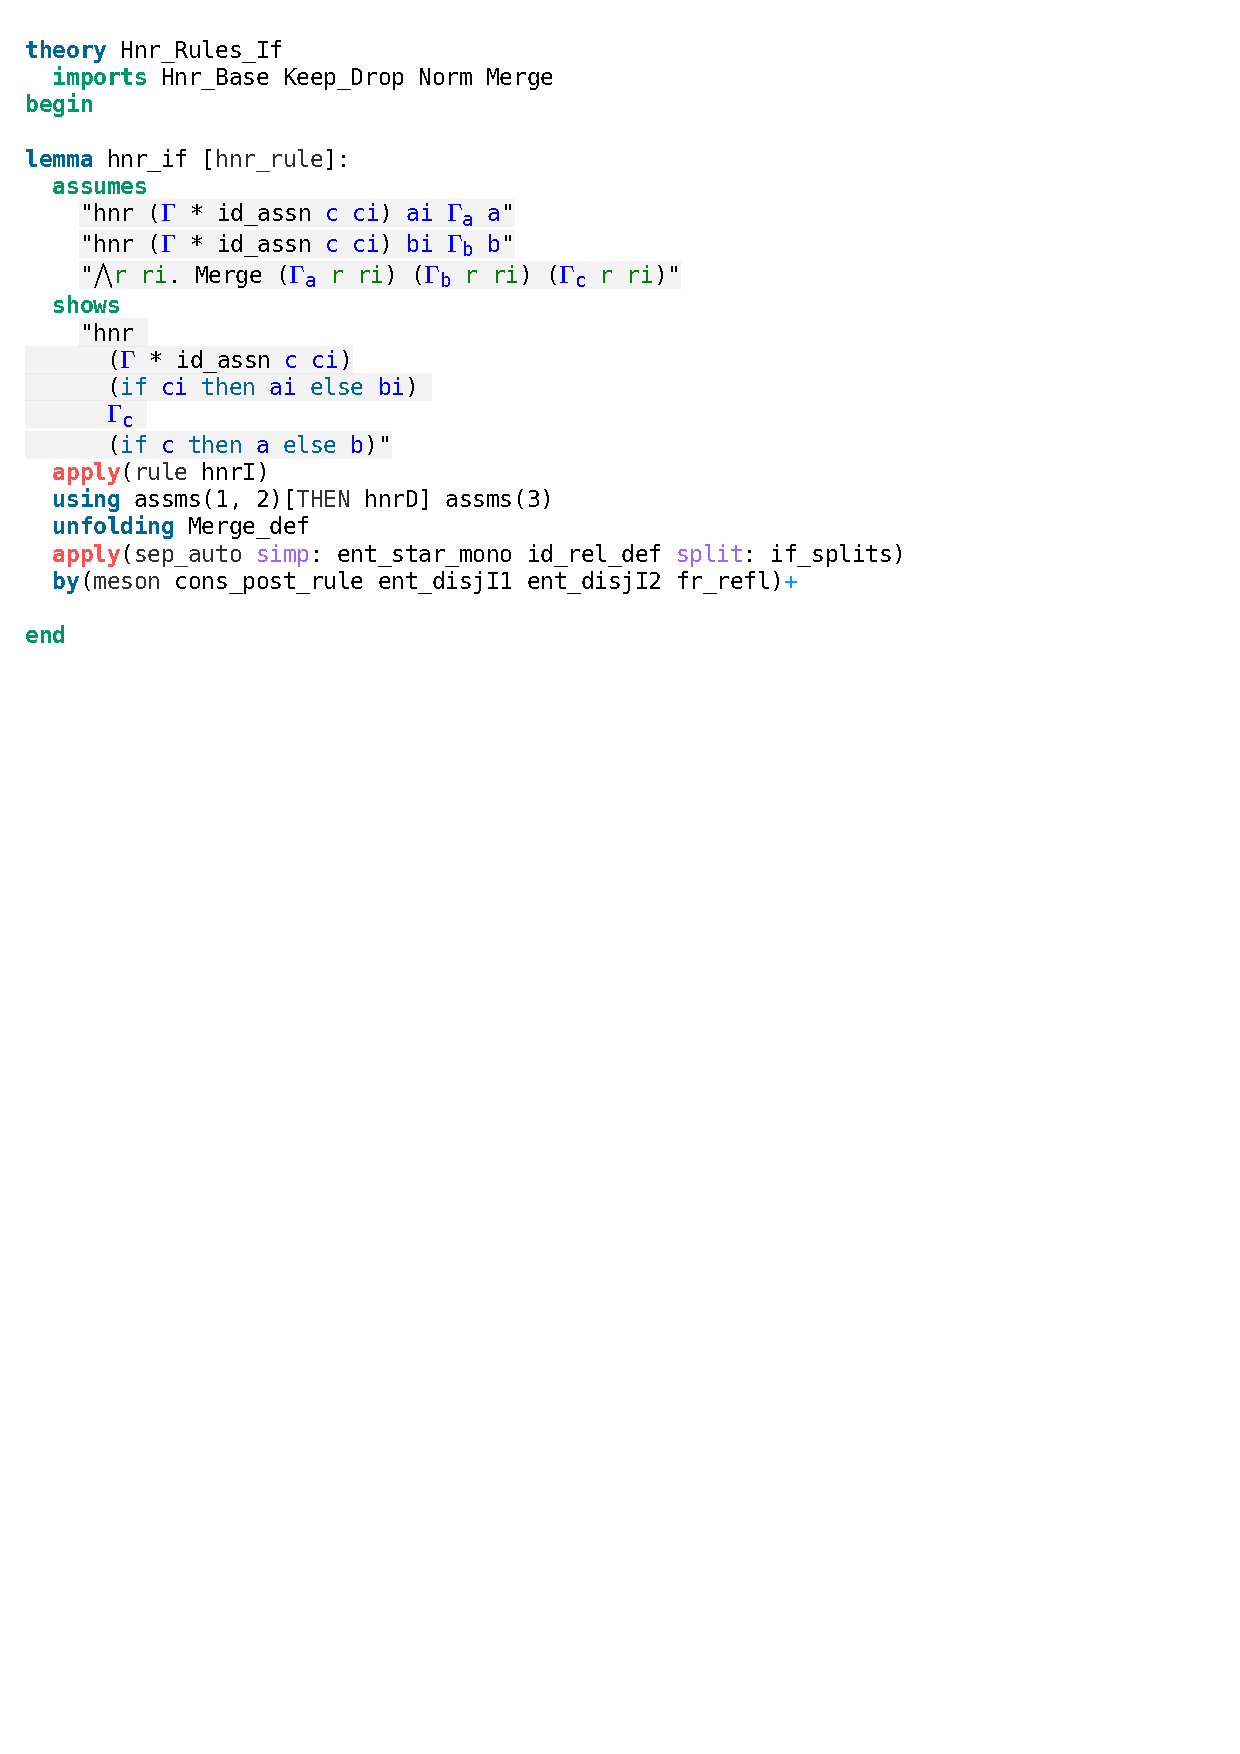
\includegraphics[trim={0 21,9cm 0 2,4cm}, clip, width=1.00\textwidth]{figures/Theory_Hnr_Rules_If.pdf}
    \caption[Hnr if rule]{Hnr if rule}
    \label{fig:hnr_if}
\end{figure}

\subsection{Case}

We defined rules for pattern matching on tuples, the sum type of the HOL library, natural numbers, and lists. They are very similar, such that we just describe them generally. In the future, we will evaluate if a general version of these rules is possible. Also, we do not yet support the conversion of case distinctions on refined types and types that contain refined types [link future work].\\
A case rule assumes the conversion of all its branches. Further, it associates keep-drop and normalization clauses with the |hnr| assumptions, such that the bound internal values of the destructured constructors, which the branches can depend on, are dropped again. Using these conversions, we can build up the case statement in the imperative program again. Therefore, the value that is pattern matched needs to be identical in both programs, shown by an identity assertion in the precondition of the |hnr| rule. Due to this, we have the deficiency of not being able to convert pattern matches on refined types, which would have different assertions.
Like in the |if| rule (\autoref{fig:hnr_if}), a last additional assumption merges the postconditions of the branches again.

\begin{figure}[htpb]
    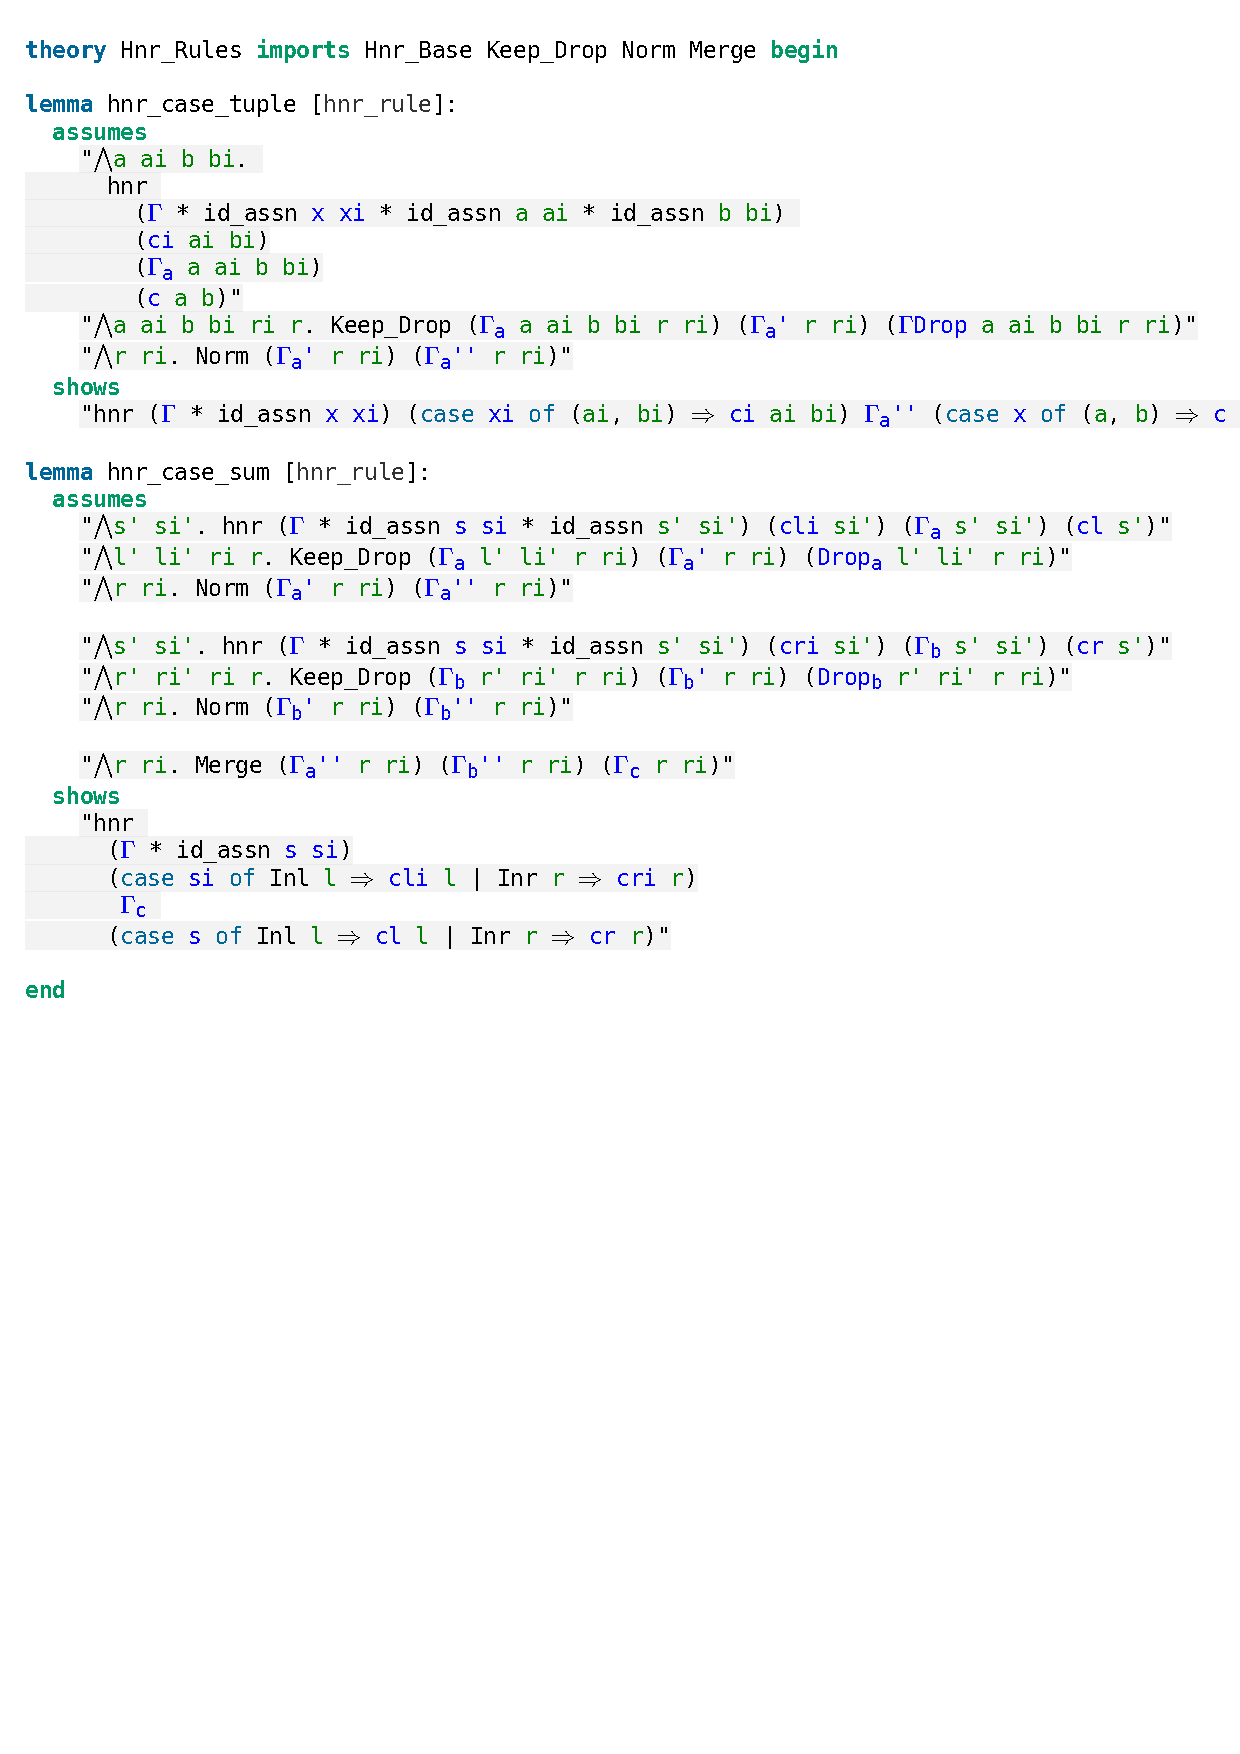
\includegraphics[trim={0 13,6cm 0 1,6cm}, clip, width=1.00\textwidth]{figures/Theory_Hnr_Rules_Case_1.pdf}
    \caption[Hnr case rules - 1]{Hnr case rules - 1}
    \label{fig:hnr_case_1}
\end{figure}

\begin{figure}[htpb]
    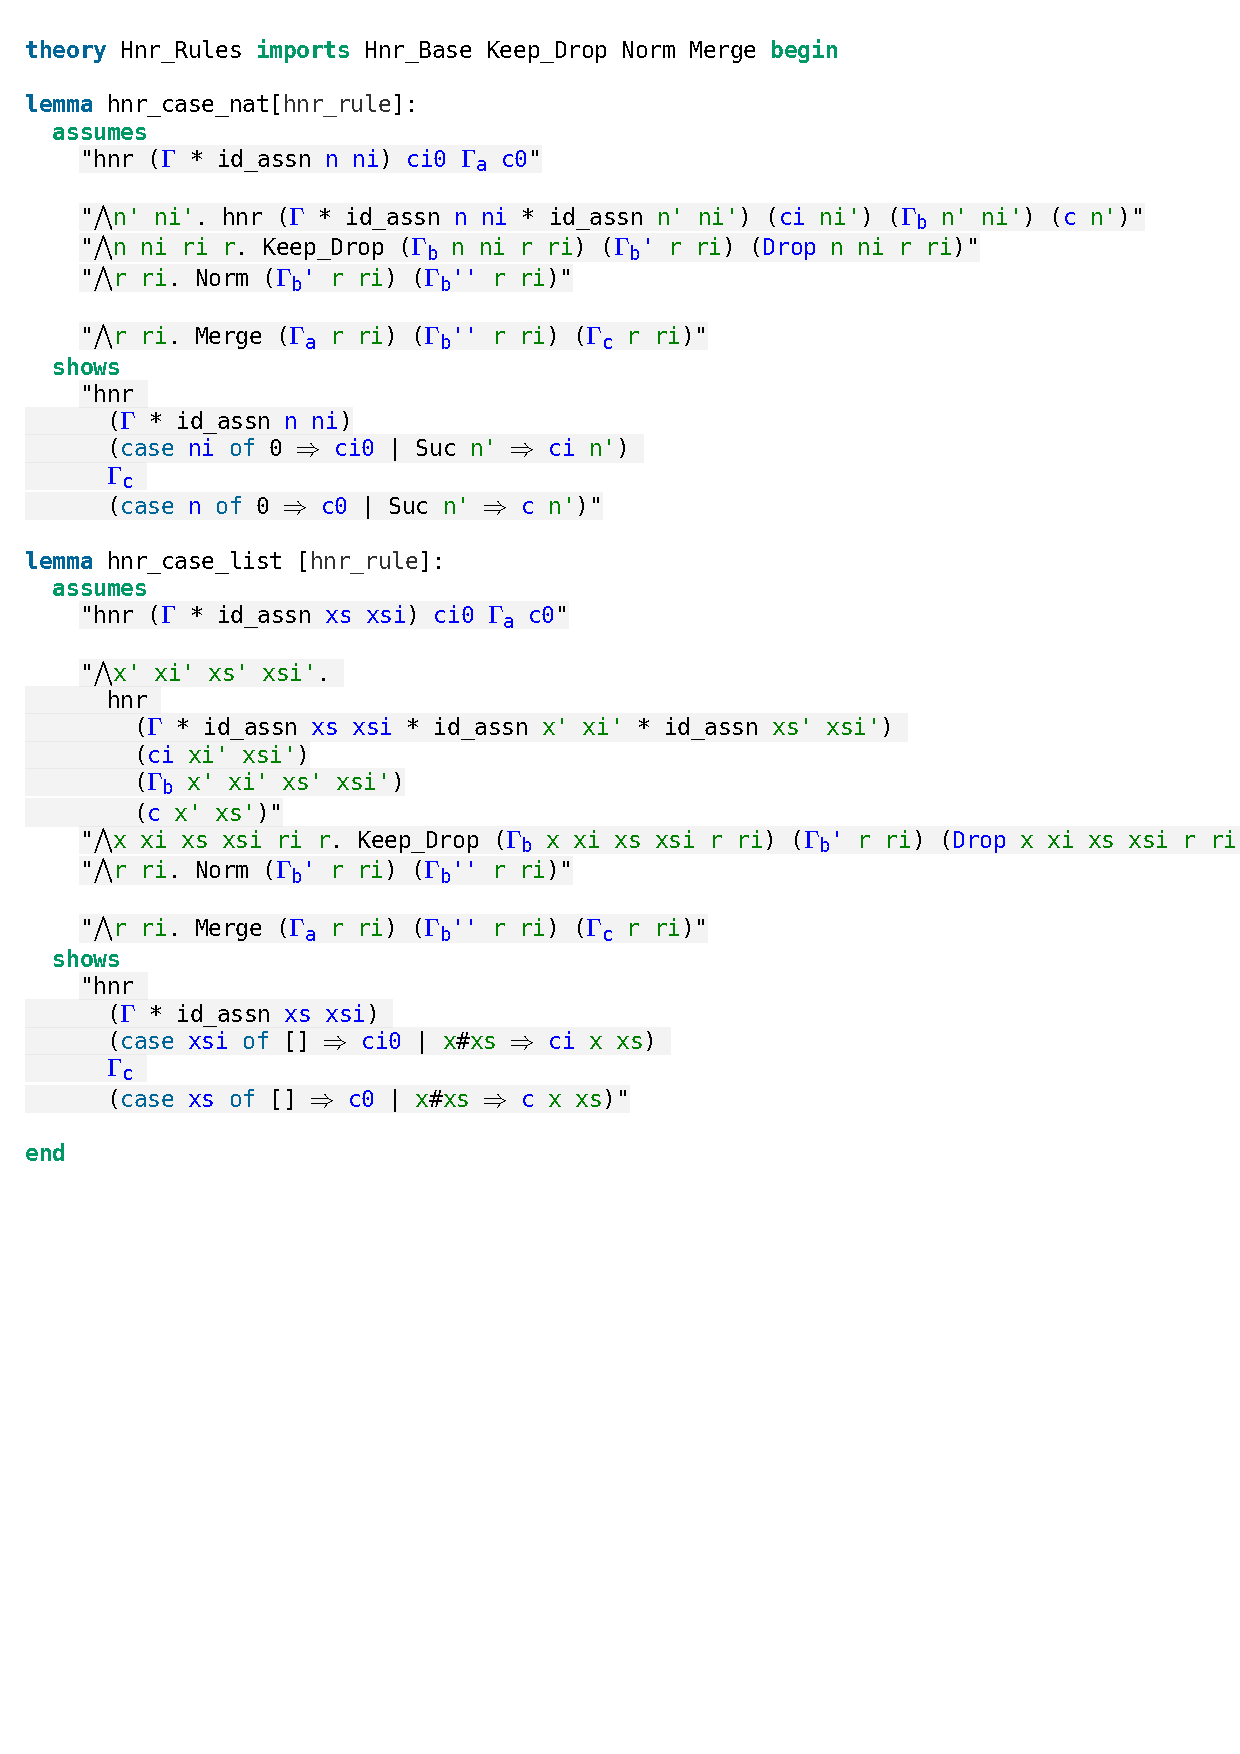
\includegraphics[trim={0 10,8cm 0 1,6cm}, clip, width=1.00\textwidth]{figures/Theory_Hnr_Rules_Case_2.pdf}
    \caption[Hnr case rules - 2]{Hnr case rules - 2}
    \label{fig:hnr_case_2}
\end{figure}

\noindent To prove the rules, we first convert the |hnr|s to Hoare triples, unfold the merge definition, and split up the conclusion into all possible cases of the pattern match using the separation logic proof automation and its |split| option. Now, we have individual goals for each case of the pattern match. We can solve these goals by using the translation assumptions of the branches and some standard rules for disjunctions of separation logic assertions. Additionally, the associated keep drop and normalization clauses help the simplifier.

\section{Fallbacks}

Expressions like |let c3 = c1 < c2| in \autoref{fig:monadified_example} cannot be translated using the constant rule (\autoref{fig:hnr_const}) since the expression is not fully evaluated, and the translation cannot depend directly on its abstraction. Theoretically, it would be possible to also monadify the less function and then translate it. However, when a expression does not contain a refined value, there is a more straightforward approach.\\
First, we can reduce such a translation to an equality assumption of the abstract and translated value, following the precondition of the |hnr| statement. Further, we can introduce an identity assertion, like in the constant rule, but we will have to prove the equality assumption in the next step (\autoref{fig:hnr_fallback}). 

\begin{figure}[htpb]
    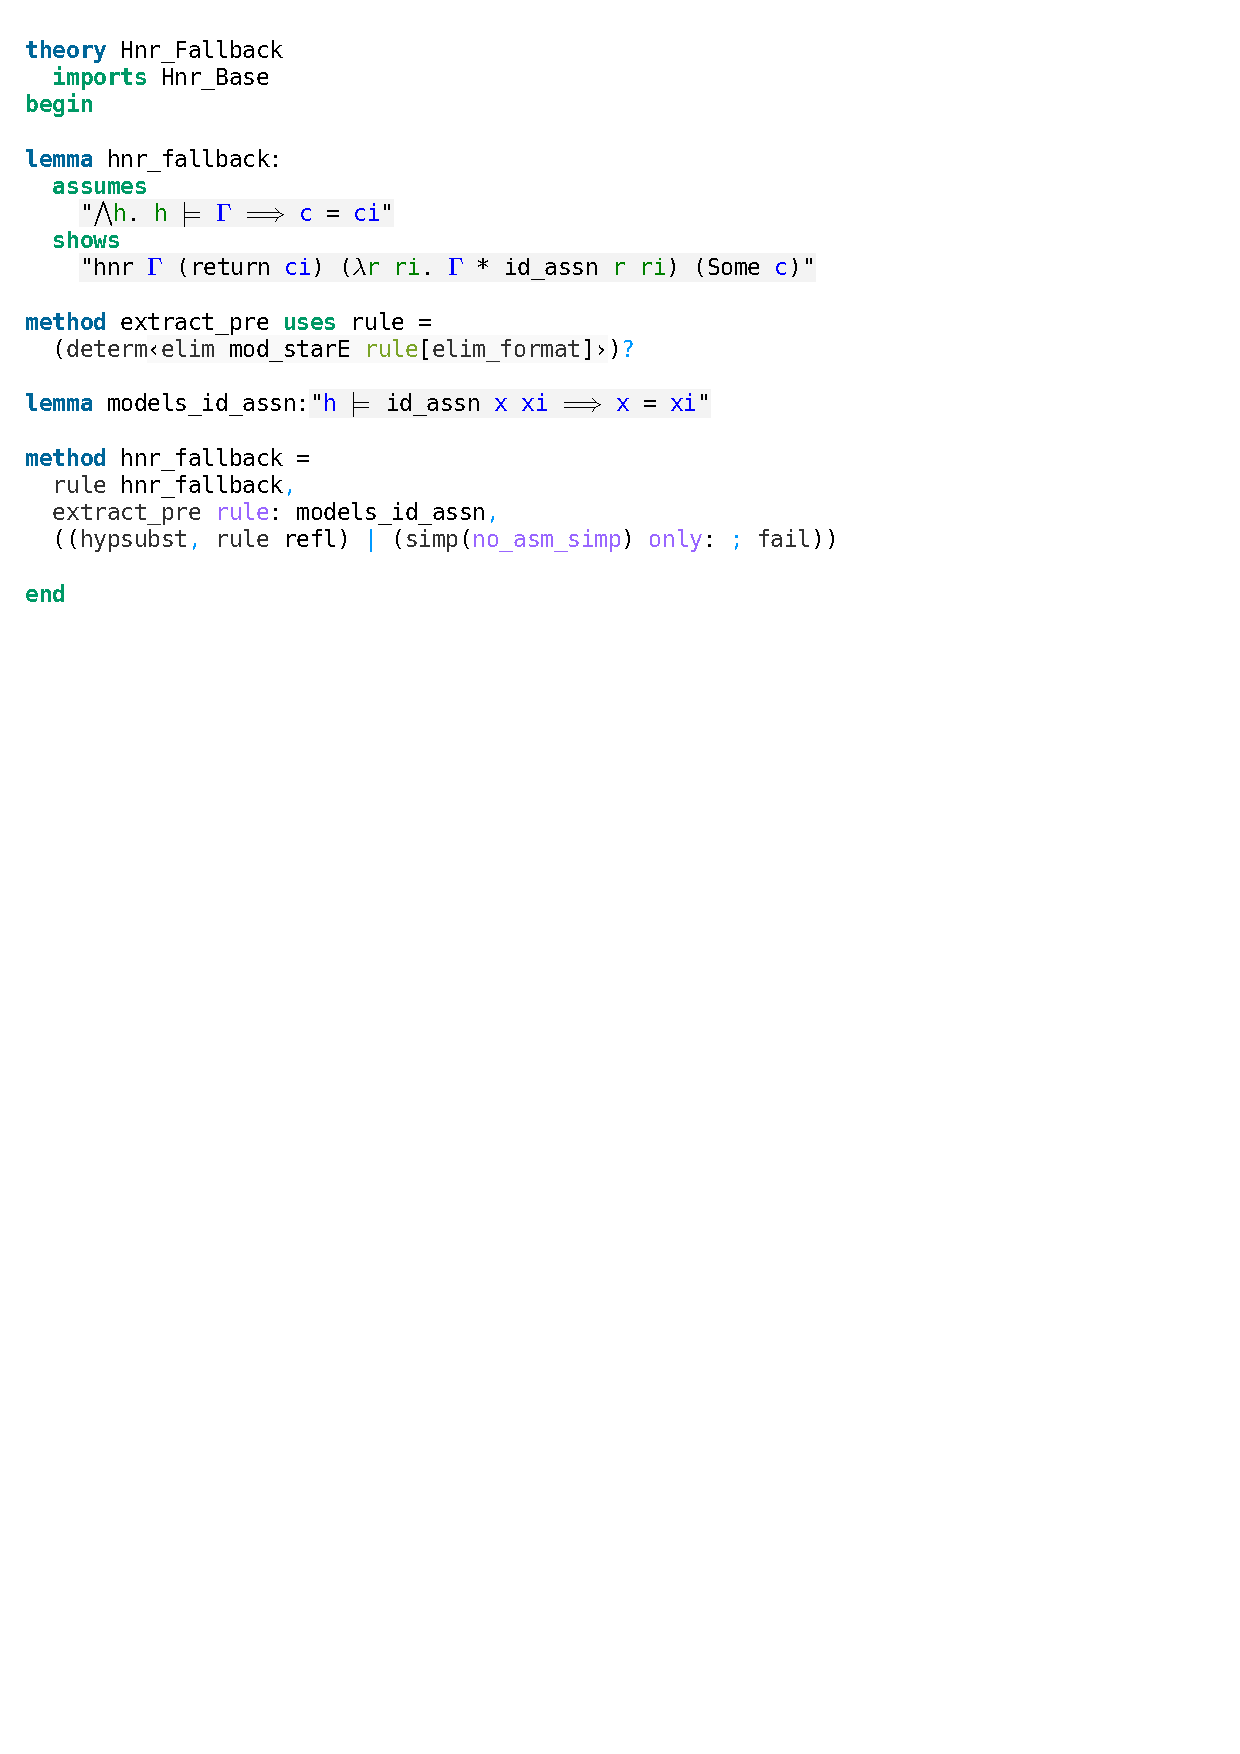
\includegraphics[trim={0 24,8cm 0 2,4cm}, clip, width=1.00\textwidth]{figures/Theory_Hnr_Fallback.pdf}
    \caption[Hnr fallback rule]{Hnr fallback rule}
    \label{fig:hnr_fallback}
\end{figure}

\noindent We can do that by substituting all the identities of the precondition. In our small example, we would substitute |c1| and |c2| with their translations, which is possible because we do not refine natural numbers and have assertions for every value.
In the final step, we can resolve the statement with simple reflexivity. We created an Eisbach method in \autoref{fig:hnr_fallback_method} for this procedure.

\begin{figure}[htpb]
    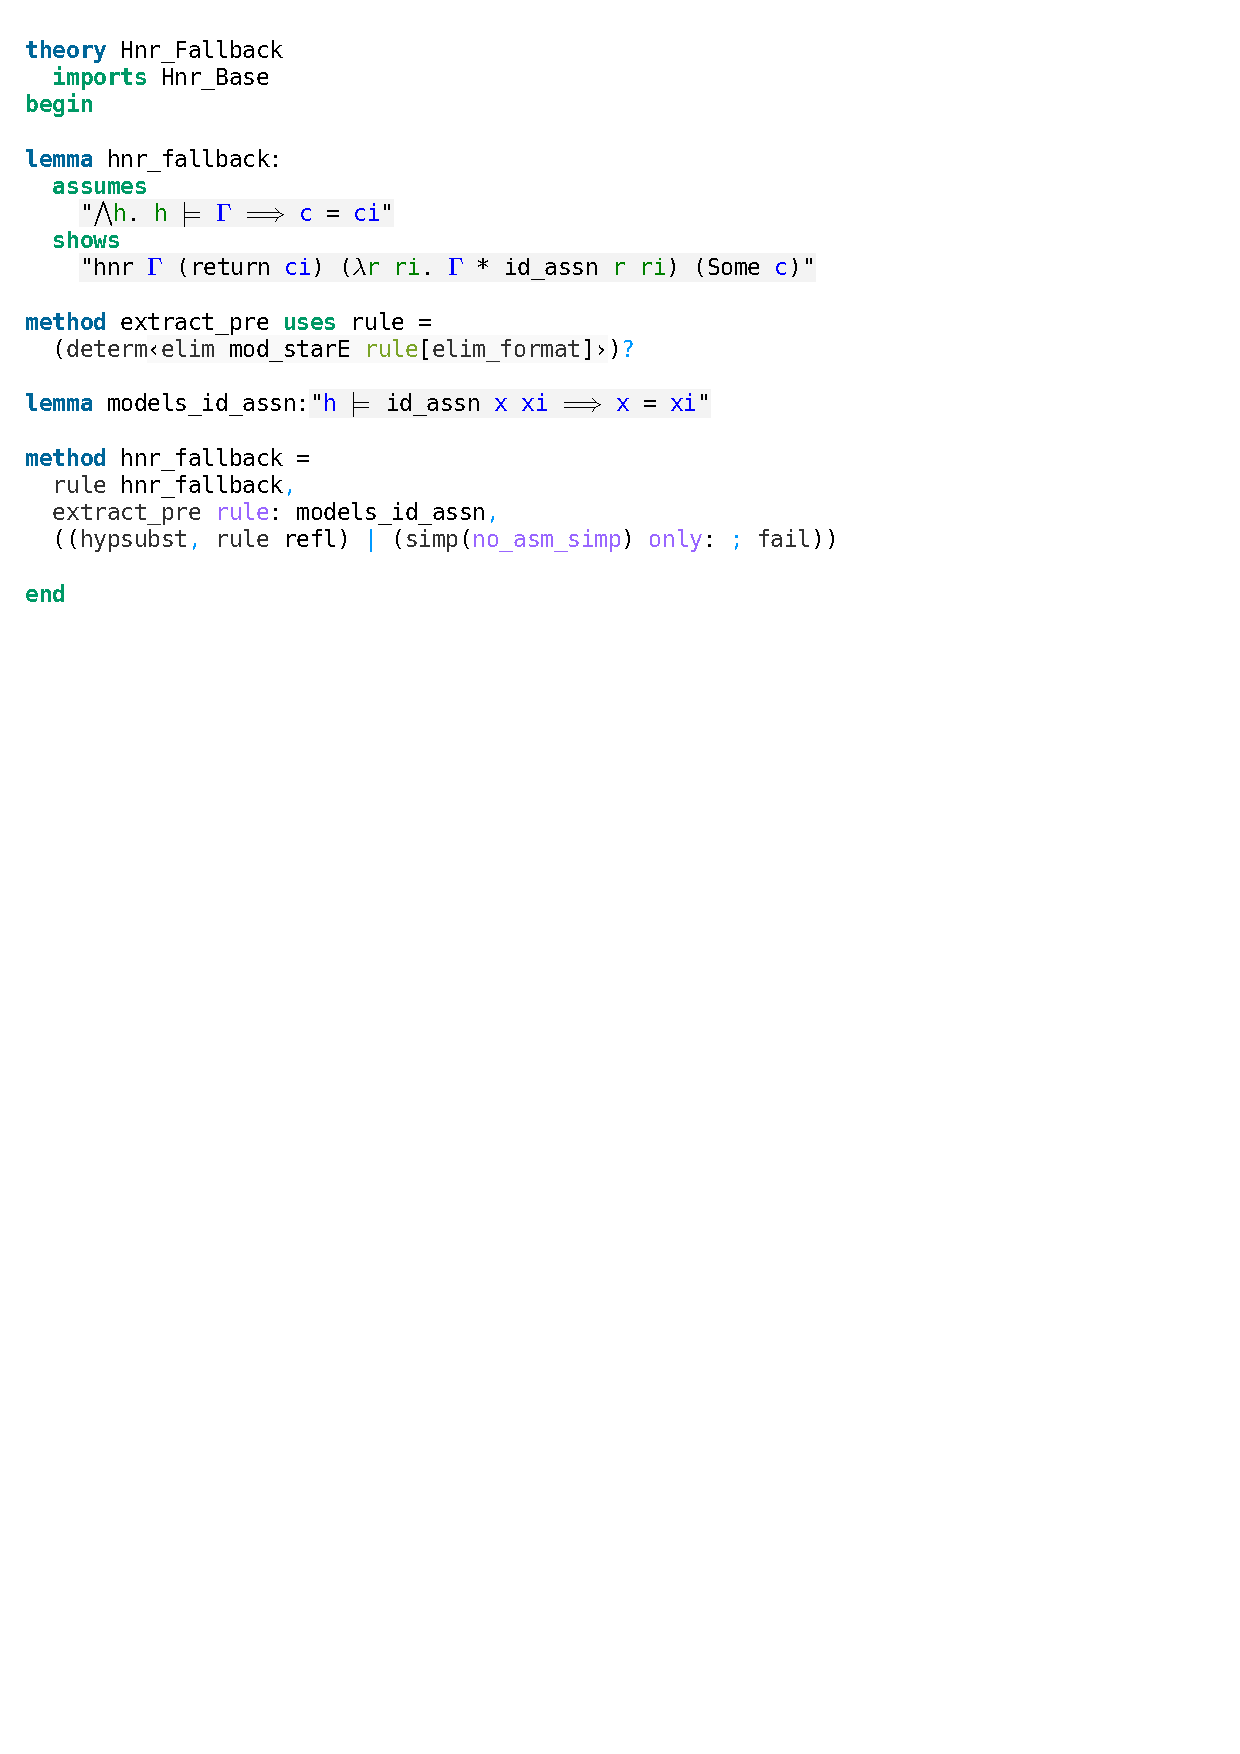
\includegraphics[trim={0 19,4cm 0 5,2cm}, clip, width=1.00\textwidth]{figures/Theory_Hnr_Fallback.pdf}
    \caption[Hnr fallback method]{Hnr fallback method}
    \label{fig:hnr_fallback_method}
\end{figure}

\section{Frame Inference}

The pre- and postconditions of the |hnr| statements during translation might not just contain the assertions needed for the translation. We will call these additional assertions \textit{frame} since they can be around the currently needed assertions. \\
Because it would be cumbersome to formulate all the |hnr| rules with this possible \textit{frame} in mind, we create a rule that automatically does so for us (\autoref{fig:hnr_frame_rule}).

\begin{figure}[htpb]
    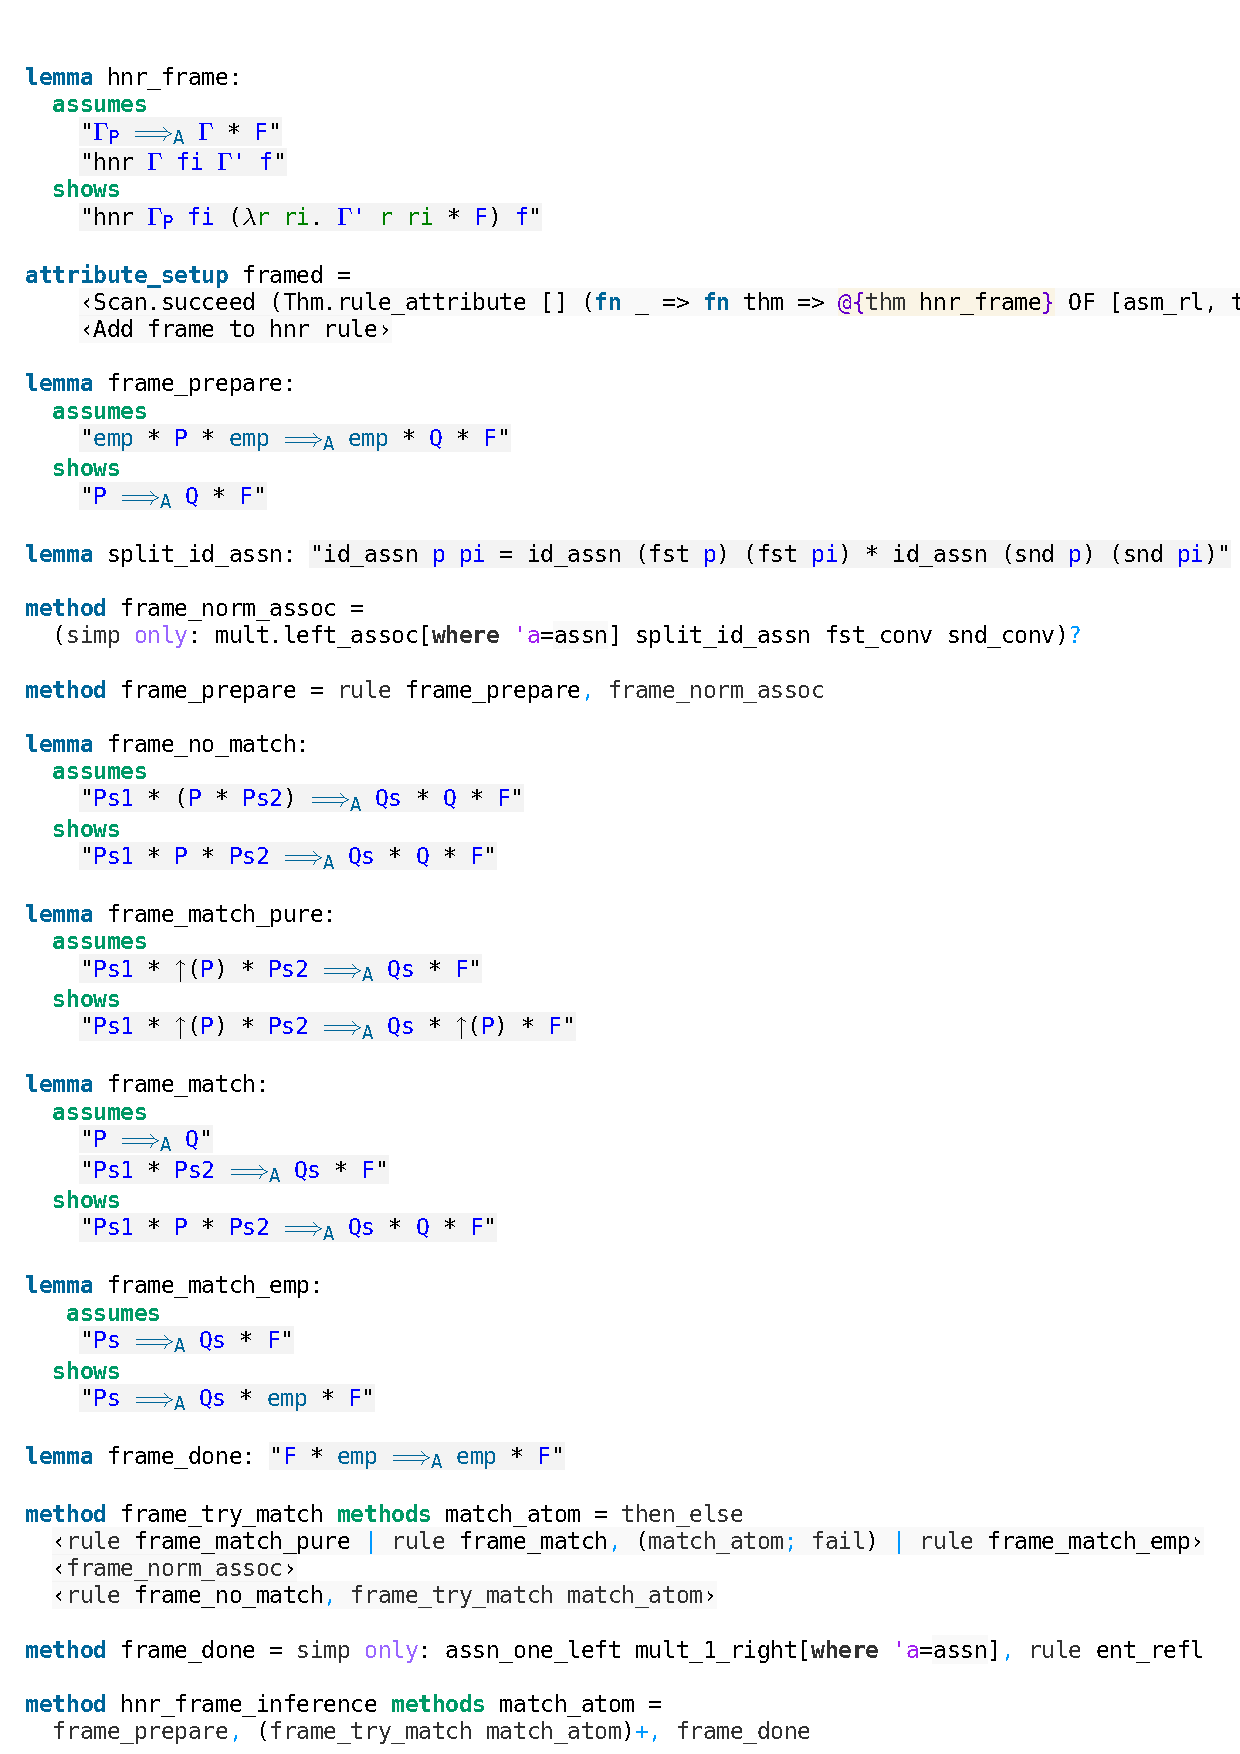
\includegraphics[trim={0 26,2cm 0 0,5cm}, clip, width=1.00\textwidth]{figures/Theory_Hnr_Frame.pdf}
    \caption[Frame rule]{Frame rule}
    \label{fig:hnr_frame_rule}
\end{figure}

\noindent It splits up the precondition into the frame and the needed assertions for proving the |hnr| statement. The frame is then passed on unchanged to the postcondition.\\
The proof of this rule can be done by translation to Hoare triples and proof automation.\\
To apply the rule conveniently, we create an attribute called |framed|. We will use this attribute, inter alia, with our previously defined pass rule (\autoref{fig:hnr_pass}) because it also needs to work if not just one identity assertion is in the precondition.
The converted pass rule looks like the following:

\begin{samepage}
\noindent $\Gamma_P \Longrightarrow_A$ |id|\_|assn x xi| $*$ |F|

\nopagebreak
\noindent $\Longrightarrow$ |hnr| $\Gamma_P$ |(return xi)| $(\lambda$ |r ri. id|\_|assn r ri| $*$ |F) (Some x)|
\end{samepage}

\noindent However, how do we identify the assertions that belong to the frame and those that are needed by the next rule? Or in other words, how do we resolve the second assumption of the frame rule?
We create a frame inference method for this purpose. The starting point is the assumption of a goal of the following form: |P| $\Longrightarrow_A$ |Q| $*$ |F|.\\
We want to split up an assertion |P| into |Q|, which the next |hnr| rule needs, and a frame |F|. Therefore, we rotate through the elements in |Q| by changing associativity stepwise from left to right. For each element, we rotate similarly through |P| until we find a matching assertion, which we then remove from |P|. The assertions which remain in |P| are consequently the frame.\\
\autoref{fig:frame_inference_example} shows an example where |P| consists of the assertions |a|, |b|, |c| and |d|, and |Q| contains |a| and |c|. By removing |a| and |c|, only |b| and |d| remain, which are the frame.

\begin{figure}[htpb]
    \centering
    |a| $*$ |b| $*$ |c| $*$ |d| $\Longrightarrow_A$ |a| $*$ |c| $*$ |?F| \\
            |b| $*$ |c| $*$ |d| $\Longrightarrow_A$ |c| $*$ |?F| \\
                    |b| $*$ |d| $\Longrightarrow_A$ |?F|
    \caption[Frame inference example]{Frame inference example}
    \label{fig:frame_inference_example}
\end{figure}

\noindent We put these steps together in a parameterized Eisbach method taking the matching strategy for assertions to also allow more sophisticated methods than simple entailment. We will use that for matching the master assertions of our diff arrays.

\section{Recursion}

We now have almost all the parts together, which we need to translate a program in the option monad to one in the heap monad. Only recursions are missing. Since we assume recursive functions using the option monad fix-point operator, we will reach a goal of the following form:\\
|hnr (|$\Gamma$ |x xi) ?c ?|$\Gamma$' |(option.fixp|\_|fun f x)|\\
|?c| is the imperative program we want to construct using the fix-point operator of the heap monad. For that, we create and prove the rule in \autoref{fig:hnr_recursion}.

\begin{figure}[htpb]
    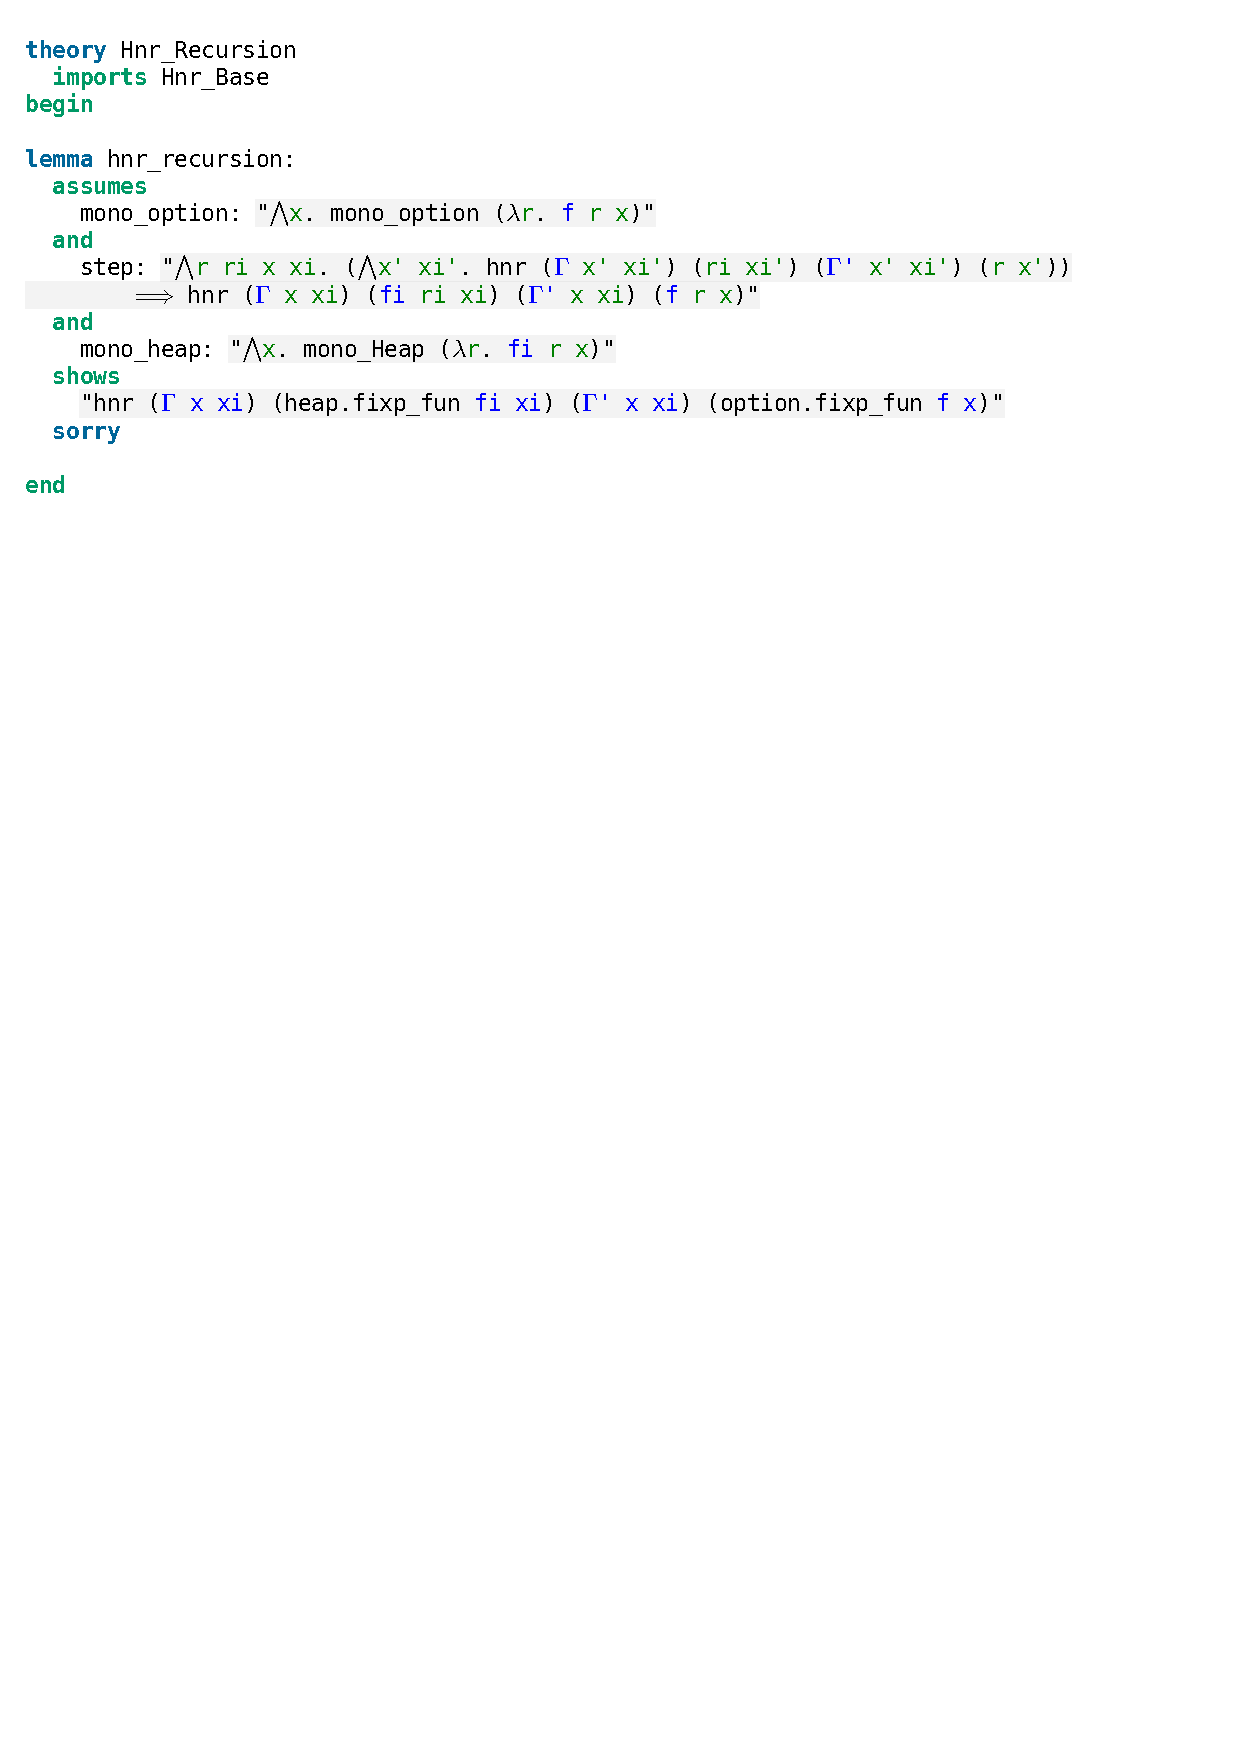
\includegraphics[trim={0 22,6cm 0 2,4cm}, clip, width=1.00\textwidth]{figures/Theory_Hnr_Recursion.pdf}
    \caption[Hnr recursion rule]{Hnr recursion rule}
    \label{fig:hnr_recursion}
\end{figure}

\noindent It states that we can construct a recursive function by assuming the |hnr| statement for the recursive call and showing that it also holds for the recursive call wrapped into the function body. Additionally, we need to assume the monotonicity of the original function and the translated function. Later on, we can show these properties automatically by using a tactic of the partial function package.\\
The application of the recursion rule is not yet fully automated, such that one needs to manually provide the pre- and postconditions [link future work]. An example is in [], where we translate the Lomuto partitioning algorithm.

\section{General Hnr Automation}\label{section:general_hnr}

Having now all the parts together, we can construct the |hnr| automation. First, we create an Eisbach method for applying the |hnr| rules we created in [hnr rules] and a custom rule set, where we will provide our (diff) array rules (\autoref{fig:hnr_rule_method}). The custom rules are applied framed with the frame inference running afterward.

\begin{figure}[htpb]
    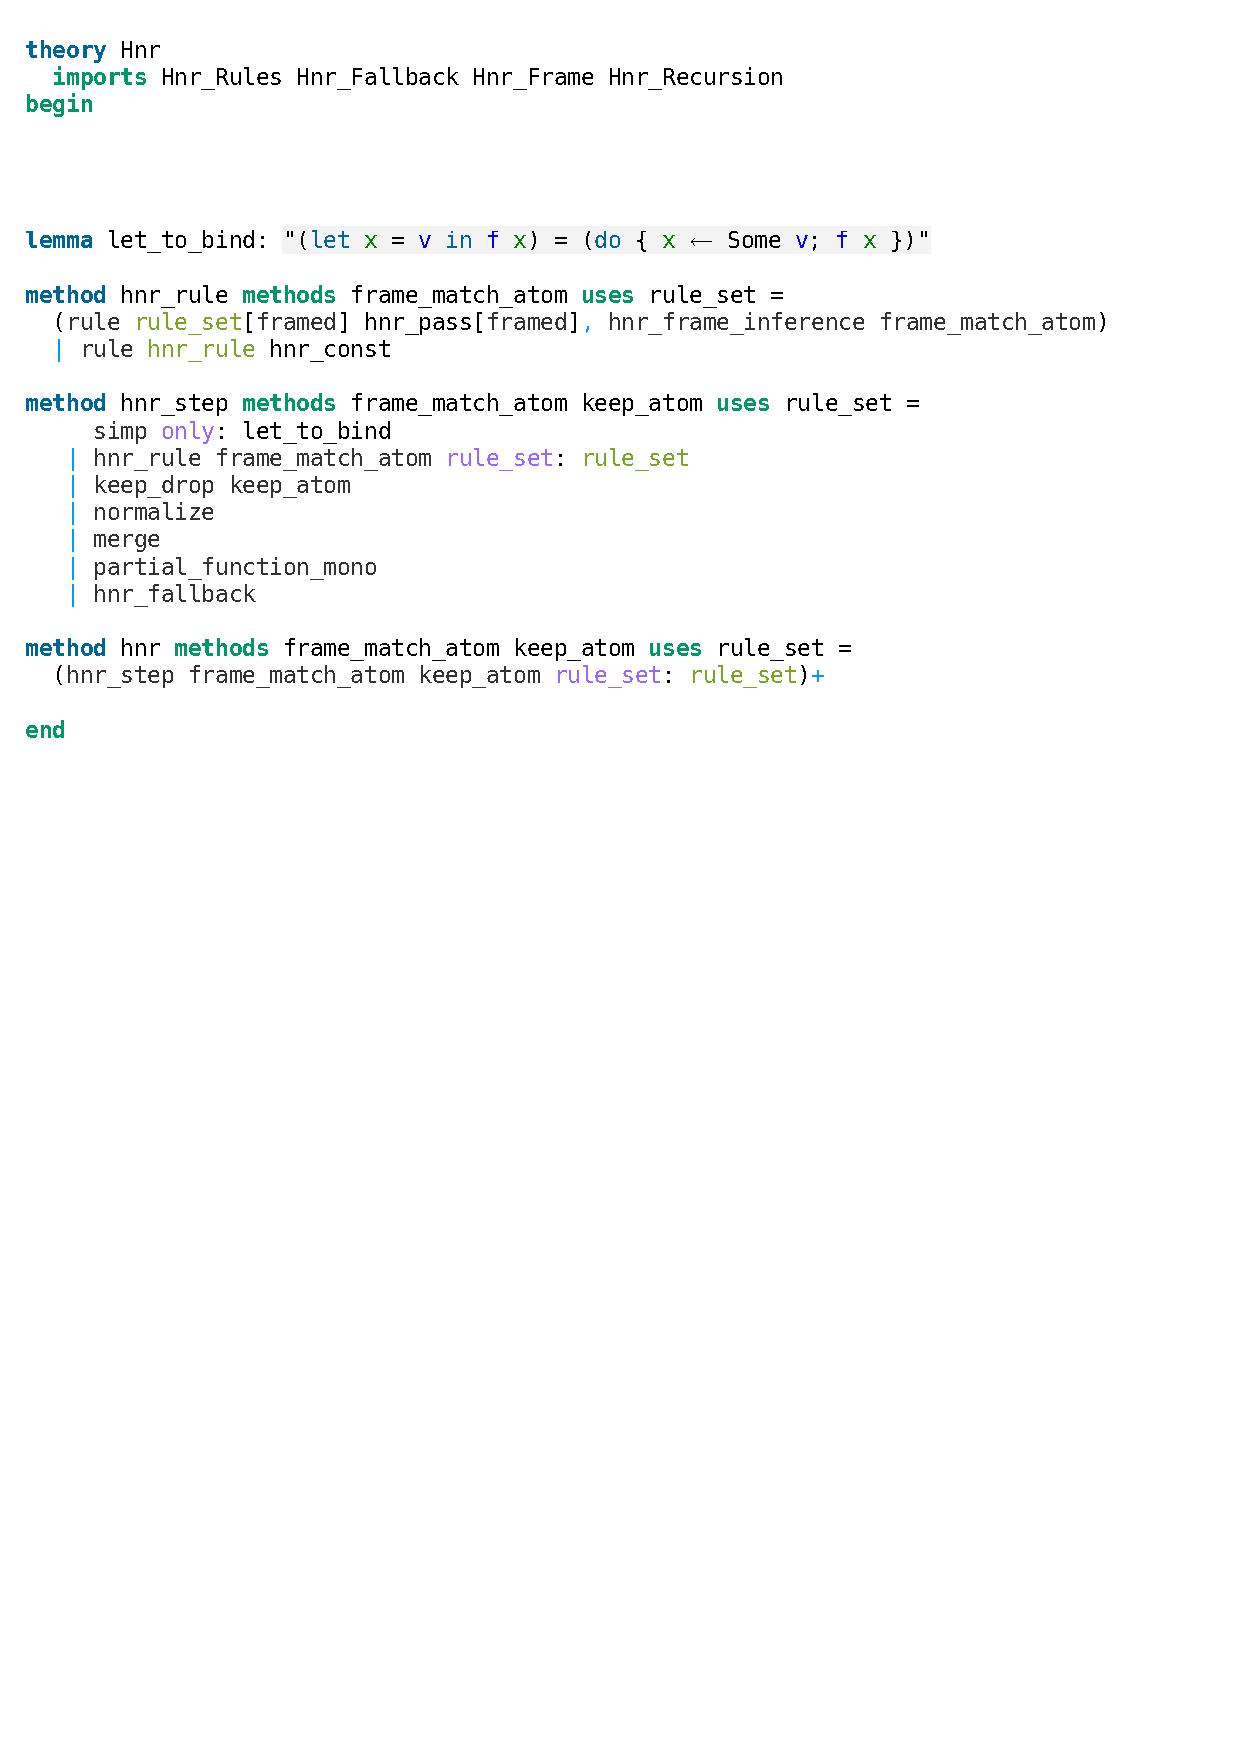
\includegraphics[trim={0 23,6cm 0 4,8cm}, clip, width=1.00\textwidth]{figures/Theory_Hnr.pdf}
    \caption[Hnr rule method]{Hnr rule method}
    \label{fig:hnr_rule_method}
\end{figure}

\noindent Next, we put the |hnr| rule, keep drop, normalize, merge, monotonicity solver, and fallback methods in this order together so that the first method that can be applied is applied (\autoref{fig:hnr_step_method}).\\
Doing this as many times as possible completes our translation automation (\autoref{fig:hnr_method}).

\begin{figure}[htpb]
    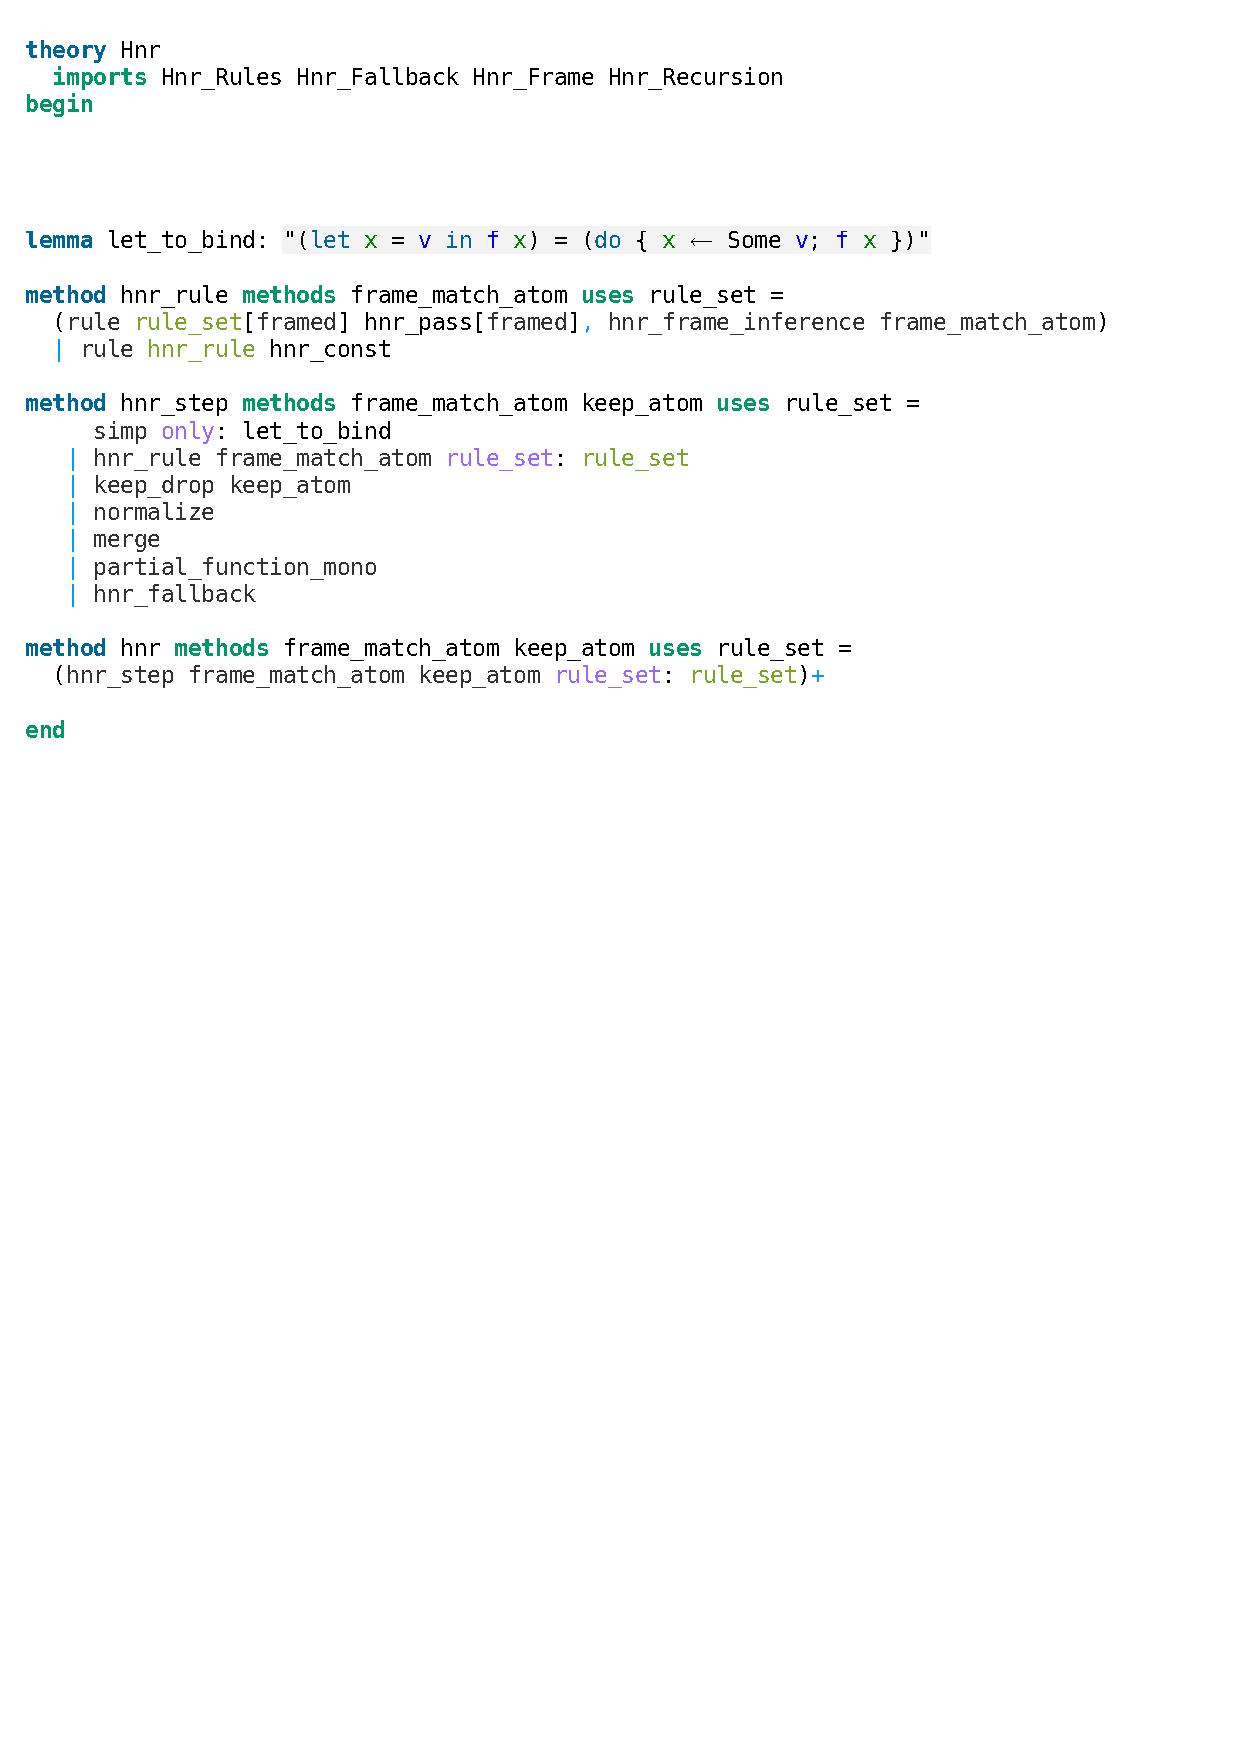
\includegraphics[trim={0 19,2cm 0 6,6cm}, clip, width=1.00\textwidth]{figures/Theory_Hnr.pdf}
    \caption[Hnr step method]{Hnr step method}
    \label{fig:hnr_step_method}
\end{figure}

\begin{figure}[htpb]
    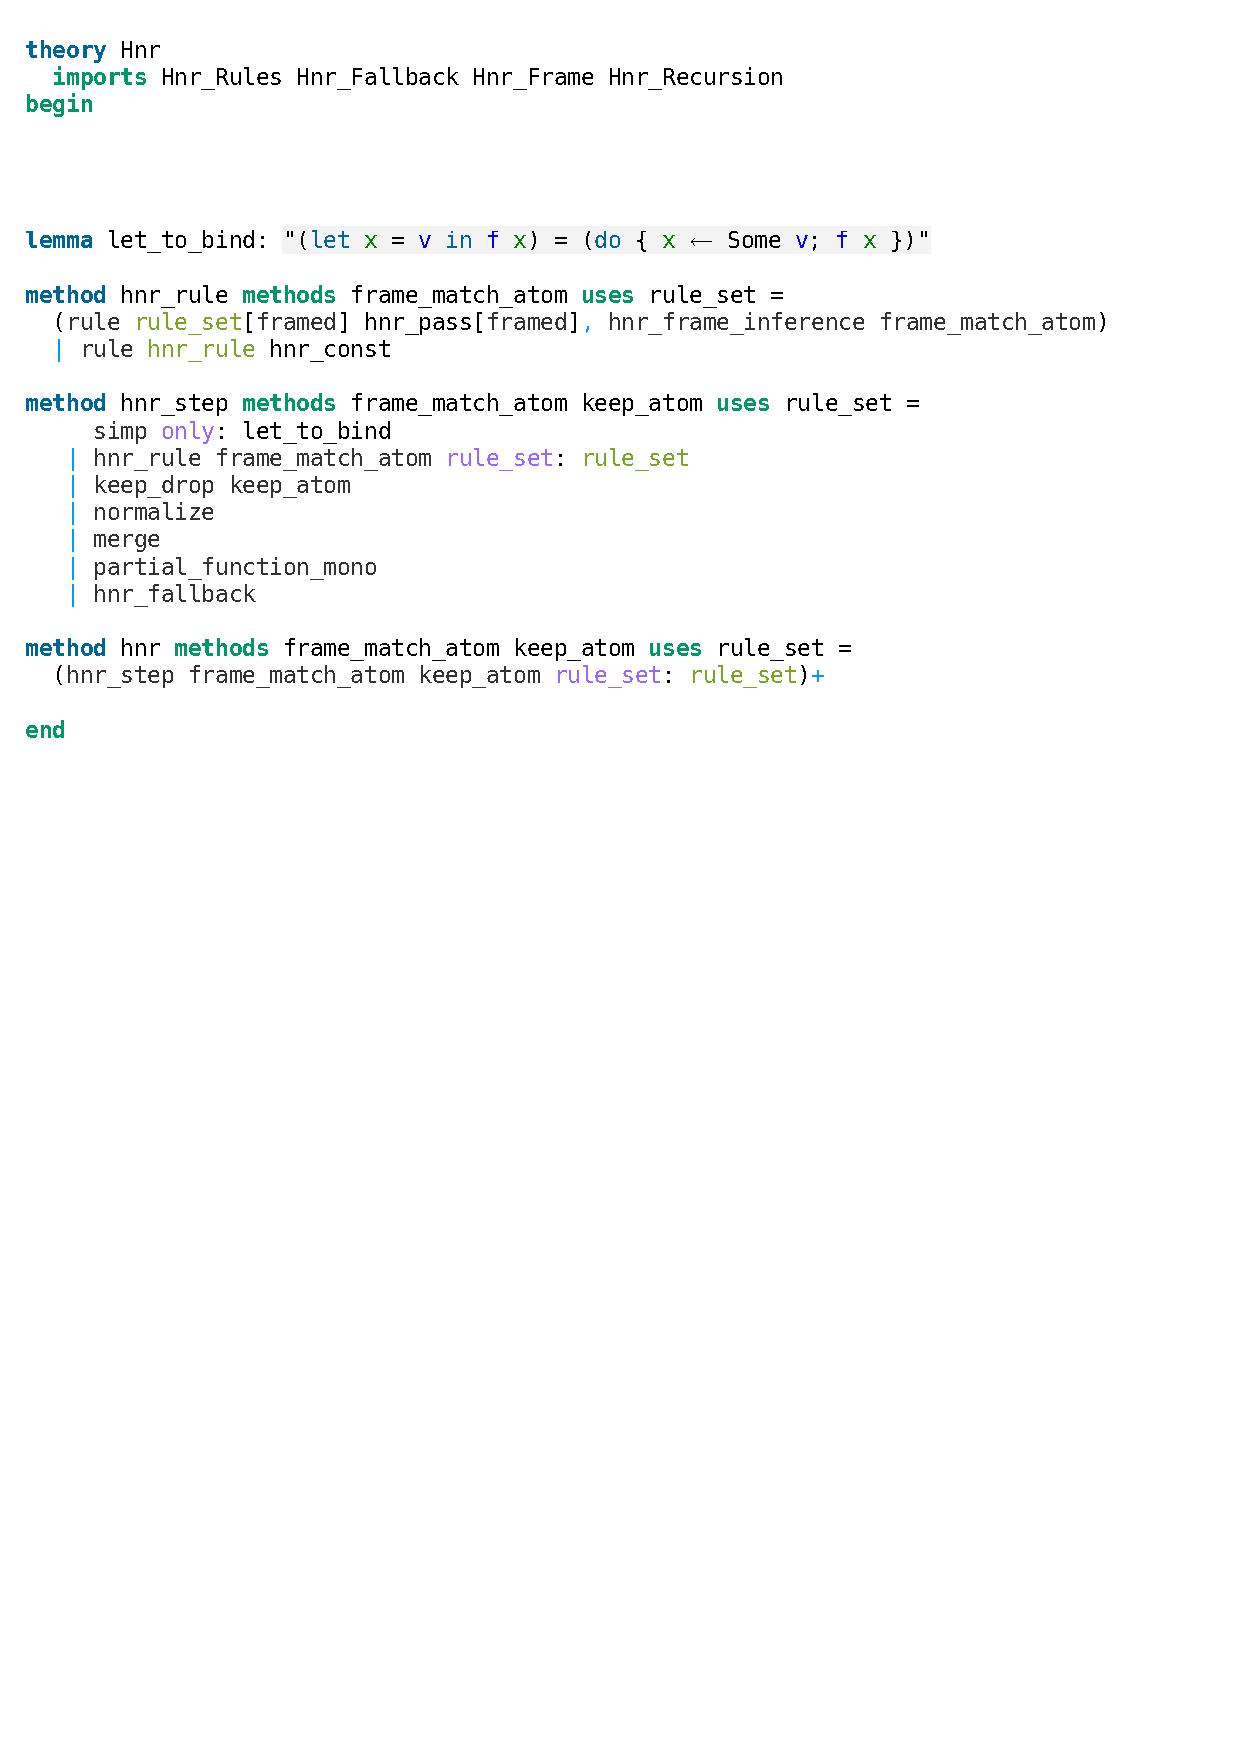
\includegraphics[trim={0 18cm 0 10,8cm}, clip, width=1.00\textwidth]{figures/Theory_Hnr.pdf}
    \caption[Hnr method]{Hnr method}
    \label{fig:hnr_method}
\end{figure}

\section{Hnr Array}

Since we do not just want to transfer programs from the option monad to the heap monad but also use the features of the heap, we will create |hnr| rules for converting lists to arrays and diff arrays (\autoref{section:hnr_diff_arr}). 
To mark lists that should be converted to arrays, we create the definition in \autoref{fig:hnr_array_marker}.

\begin{figure}[htpb]
    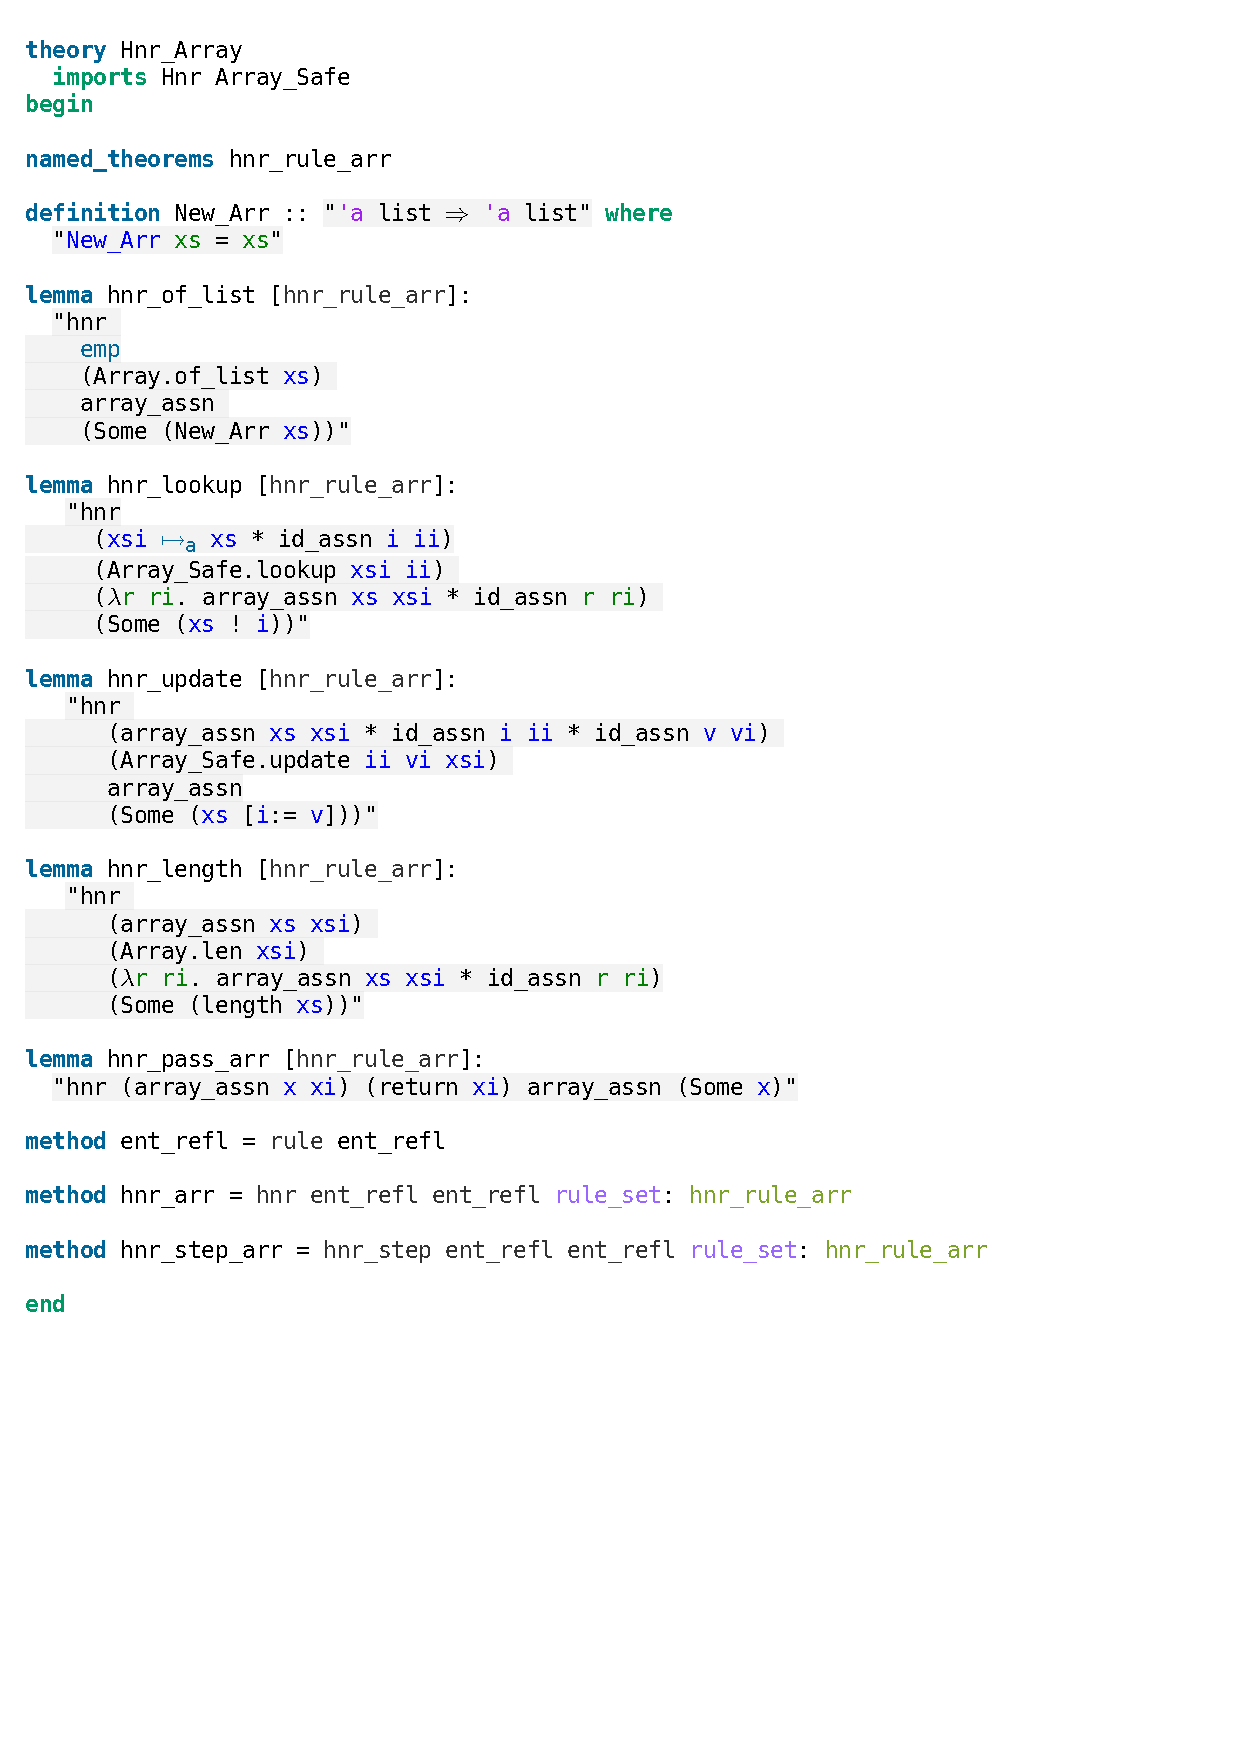
\includegraphics[trim={0 25,4cm 0 3,4cm}, clip, width=1.00\textwidth]{figures/Theory_Hnr_Array.pdf}
    \caption[Hnr array marker]{Hnr array marker}
    \label{fig:hnr_array_marker}
\end{figure}

\noindent If we reach such a definition, we create an array and introduce an array assertion using the rule in \autoref{fig:hnr_array_constructor}.

\begin{figure}[htpb]
    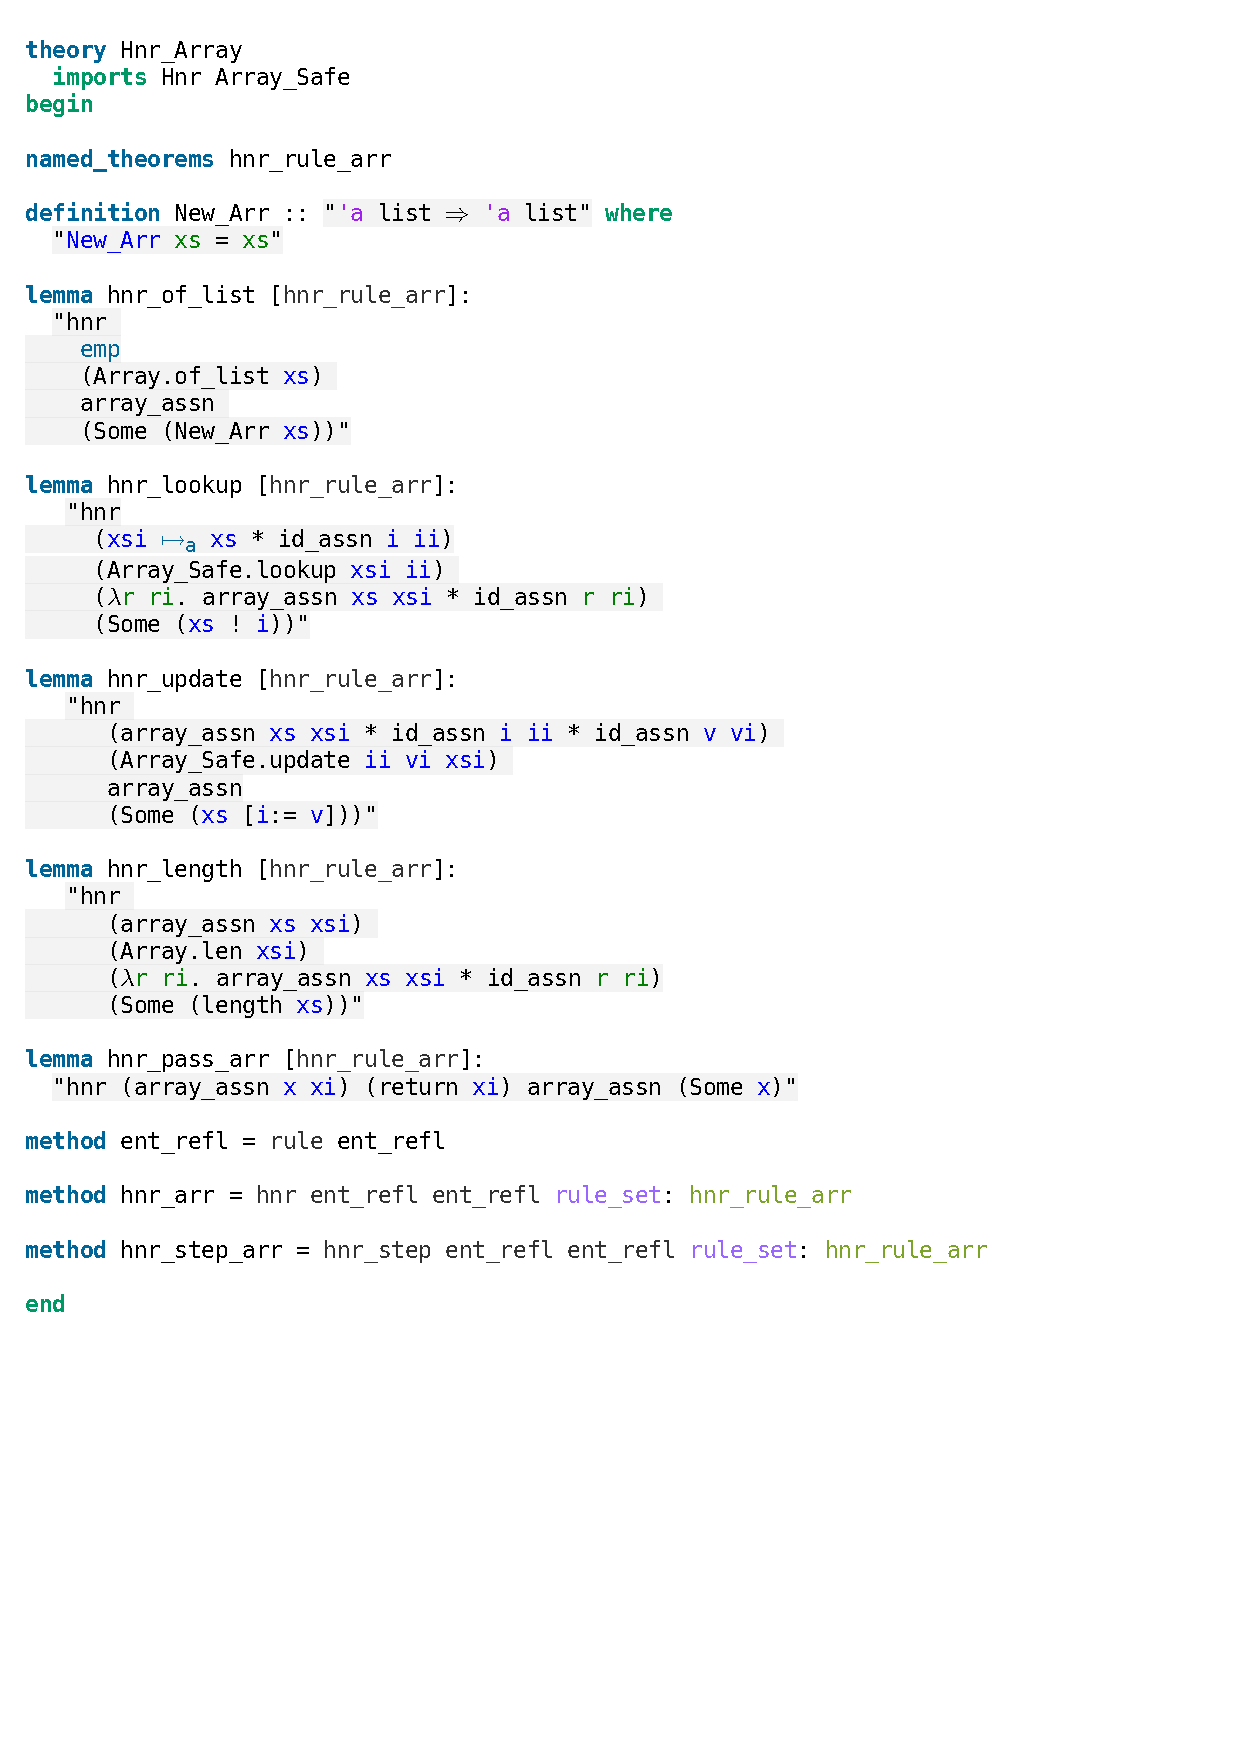
\includegraphics[trim={0 22,1cm 0 4,8cm}, clip, width=1.00\textwidth]{figures/Theory_Hnr_Array.pdf}
    \caption[Hnr array constructor]{Hnr array constructor}
    \label{fig:hnr_array_constructor}
\end{figure}

\noindent We collect the array rules in a rule set called |hnr|\_|rule|\_|arr|, which we then pass on to the |hnr| automation methods. The other rules are similarly straightforward and follow the rule of having an assertion for every variable in the program. Moreover, they use safe versions of the standard array operation of Imperative/HOL, which we created analogous to the safe versions of the diff array operations (\autoref{section:safe_diff_arr}), so we do not have to deal with the bounds of the arrays.

\begin{figure}[htpb]
    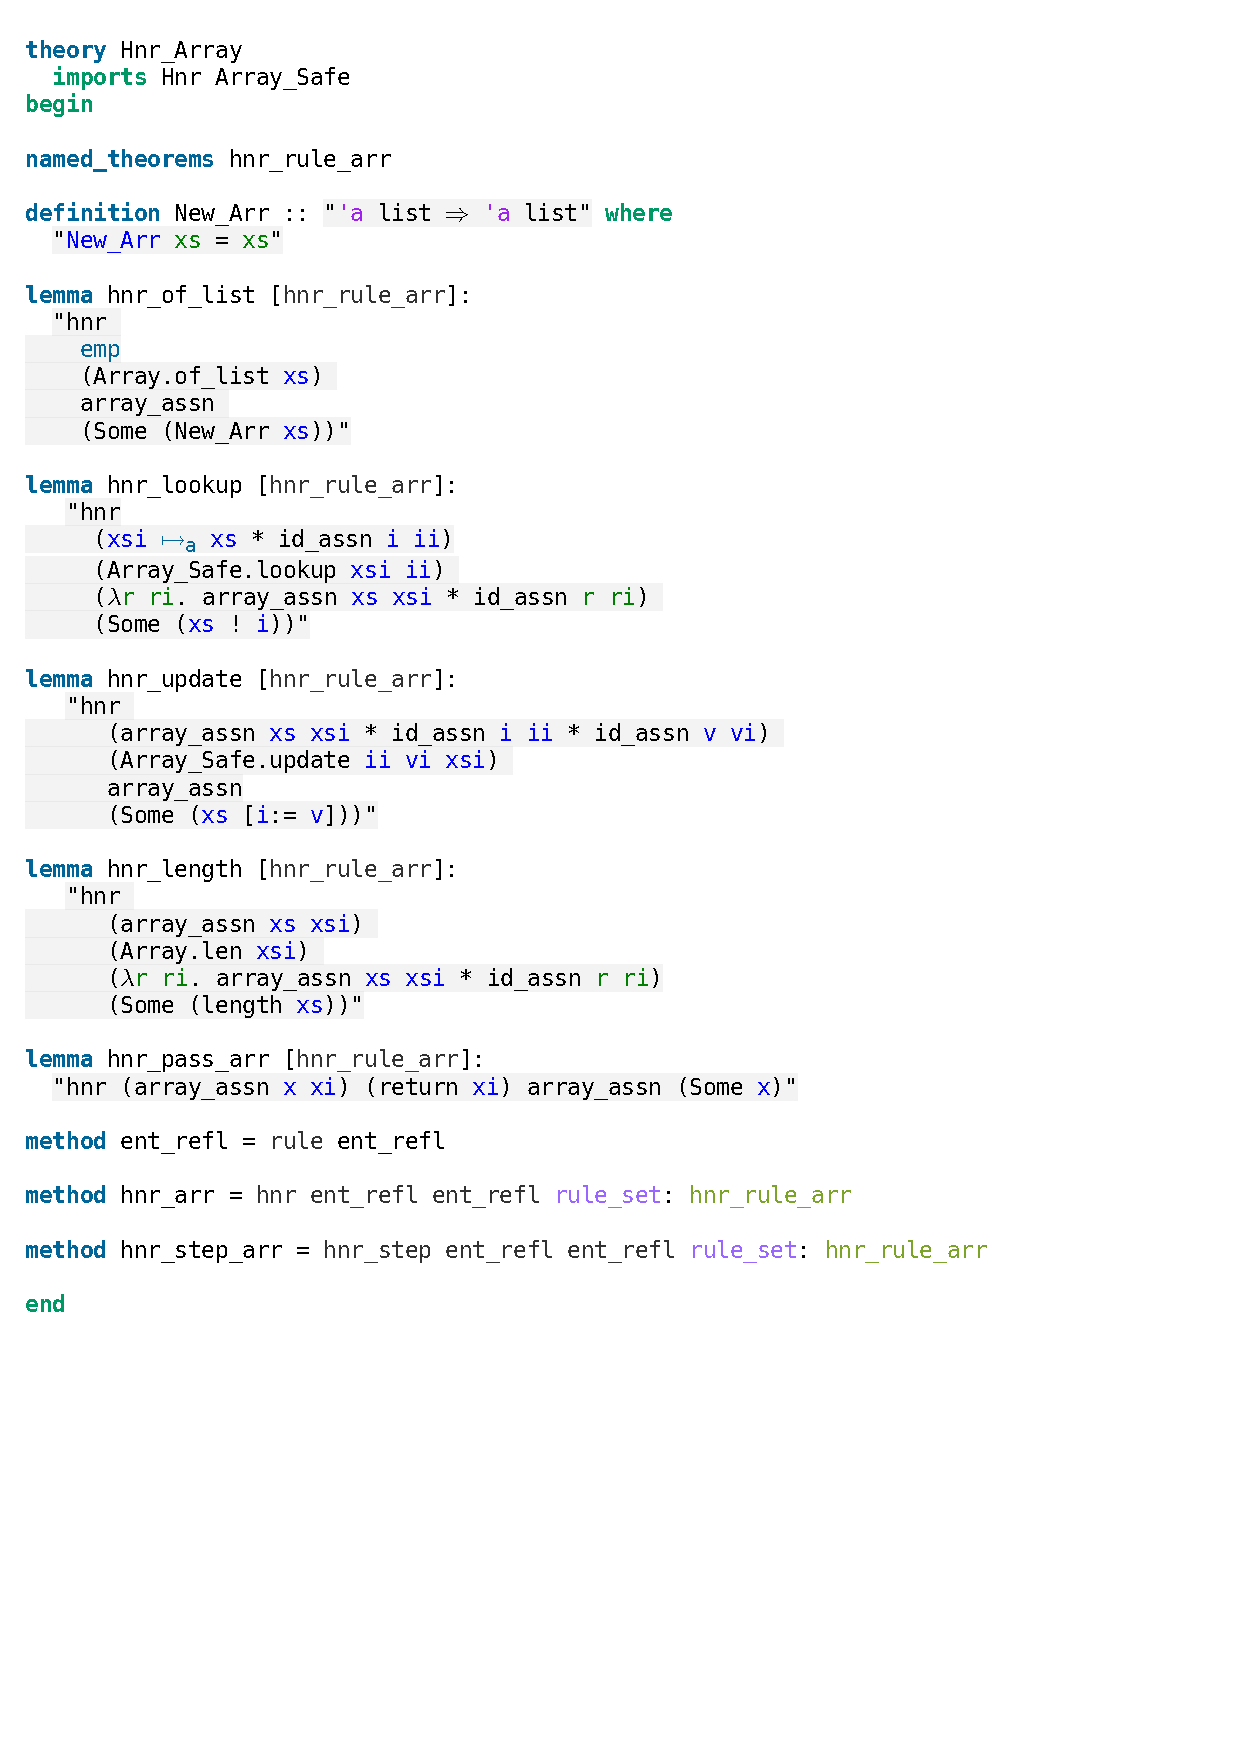
\includegraphics[trim={0 11cm 0 8cm}, clip, width=1.00\textwidth]{figures/Theory_Hnr_Array.pdf}
    \caption[Hnr array rules]{Hnr array rules}
    \label{fig:hnr_array_rules}
\end{figure}

\noindent All the rules can be directly proven by converting the |hnr| statements to Hoare triples and then using the separation logic proof automation. Moreover, by passing the rule set to the |hnr| proof automation (\autoref{section:general_hnr}) and using entailment reflexivity as strategies for the frame inference and keep drop method, we can finally convert programs using lists to arrays with verified equivalence.

\begin{figure}[htpb]
    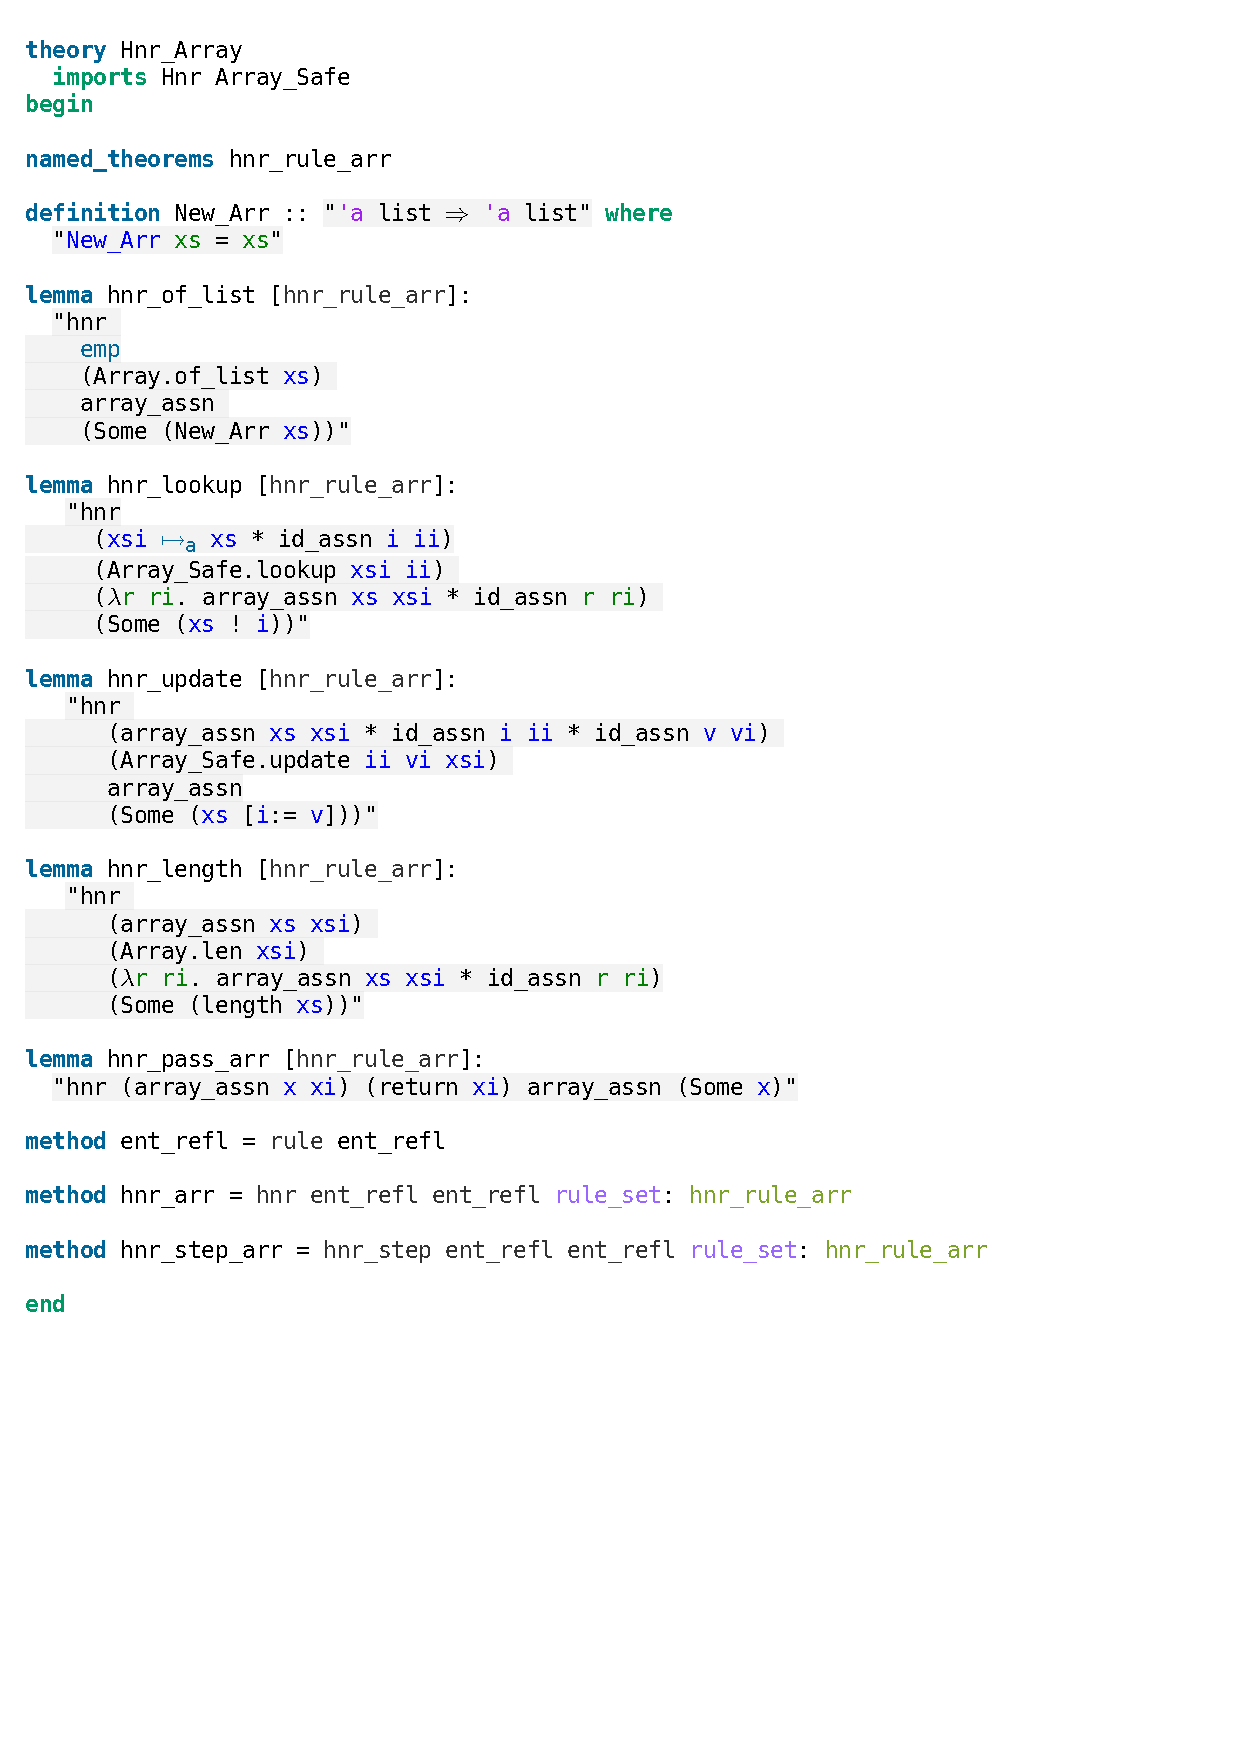
\includegraphics[trim={0 9,2cm 0 19cm}, clip, width=1.00\textwidth]{figures/Theory_Hnr_Array.pdf}
    \caption[Hnr array method]{Hnr array method}
    \label{fig:hnr_array_method}
\end{figure}

\noindent As an example, we translate \autoref{fig:monadified_example}, which results in \autoref{fig:hnr_array_example}, where the list length operation and the list update operations are replaced with the corresponding array operations.

\begin{figure}[htpb]
    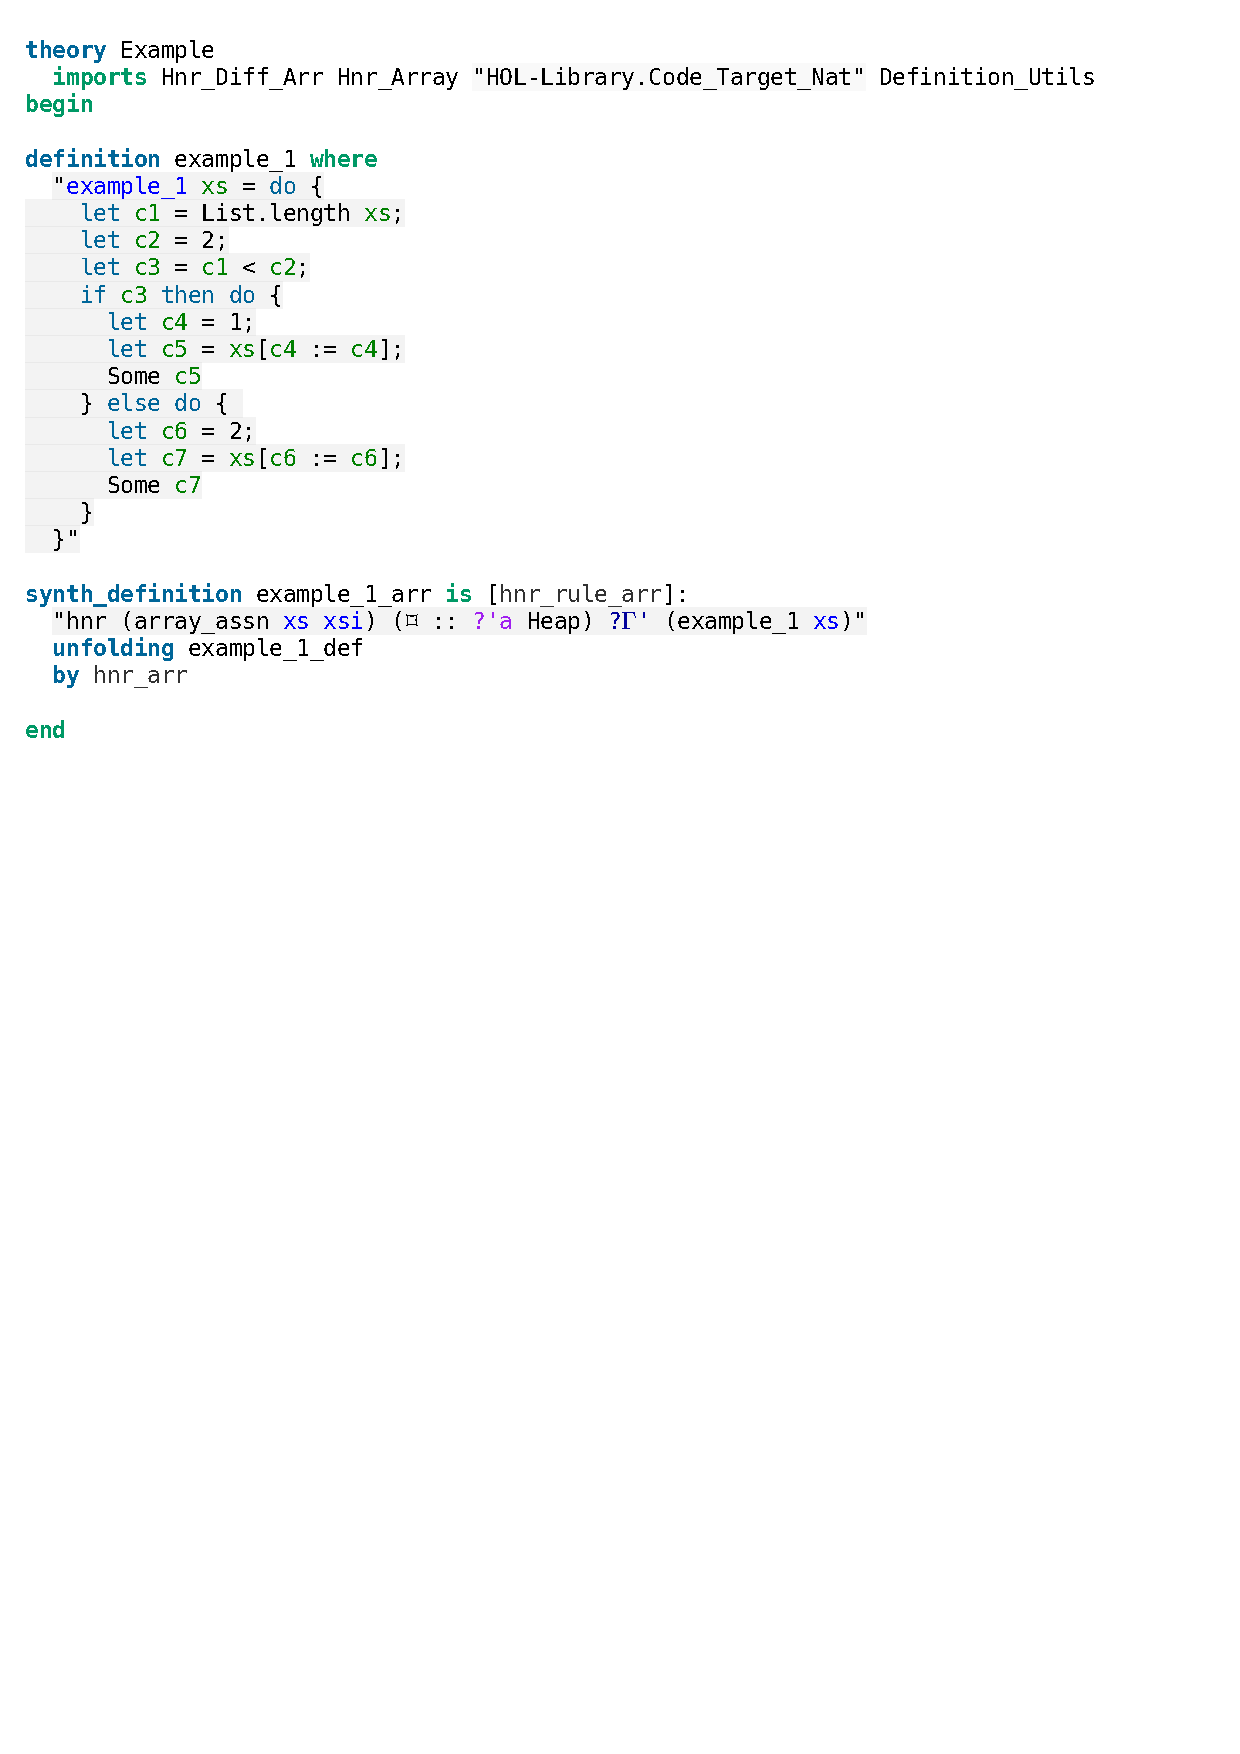
\includegraphics[trim={0 18cm 0 9,8cm}, clip, width=1.00\textwidth]{figures/Theory_Example.pdf}
    {
    \footnotesize
    |Output:|\\
    |example|\_|1|\_|arr| $\equiv$ \\
    |Array|.|len xsi >>=| \\
    |(|$\lambda$|x. return 2 >>=| \\
    |   (|$\lambda$|xa. return (x < xa) >>=| \\
    |       (|$\lambda$|x. if x| \\
    |           then return 1 >>=| \\
    |               (|$\lambda$|x. Array|\_|Safe.update x x xsi >>= return)| \\
    |           else return 2 >>=| \\
    |               (|$\lambda$|x. Array|\_|Safe.update x x xsi >>= return)|\\
    |       )|\\
    |    )|\\
    |)|
    }
    
    \caption[Example translation to arrays]{Example translation to arrays}
    \label{fig:hnr_array_example}
\end{figure}

\noindent More examples are in the theory |Test|\_|Hnr|.|thy|. \\
The conversion works unless the list is used in a non-linear way since arrays are ephemeral. To also cover this case, we will use diff arrays. 

\section{Hnr Diff Array}\label{section:hnr_diff_arr}

The |hnr| rules for diff arrays are analogous to the array ones, except for the array assertion, instead of which we use a new version of the master assertion (\autoref{fig:hnr_master_assn}). 

\begin{figure}[htpb]
    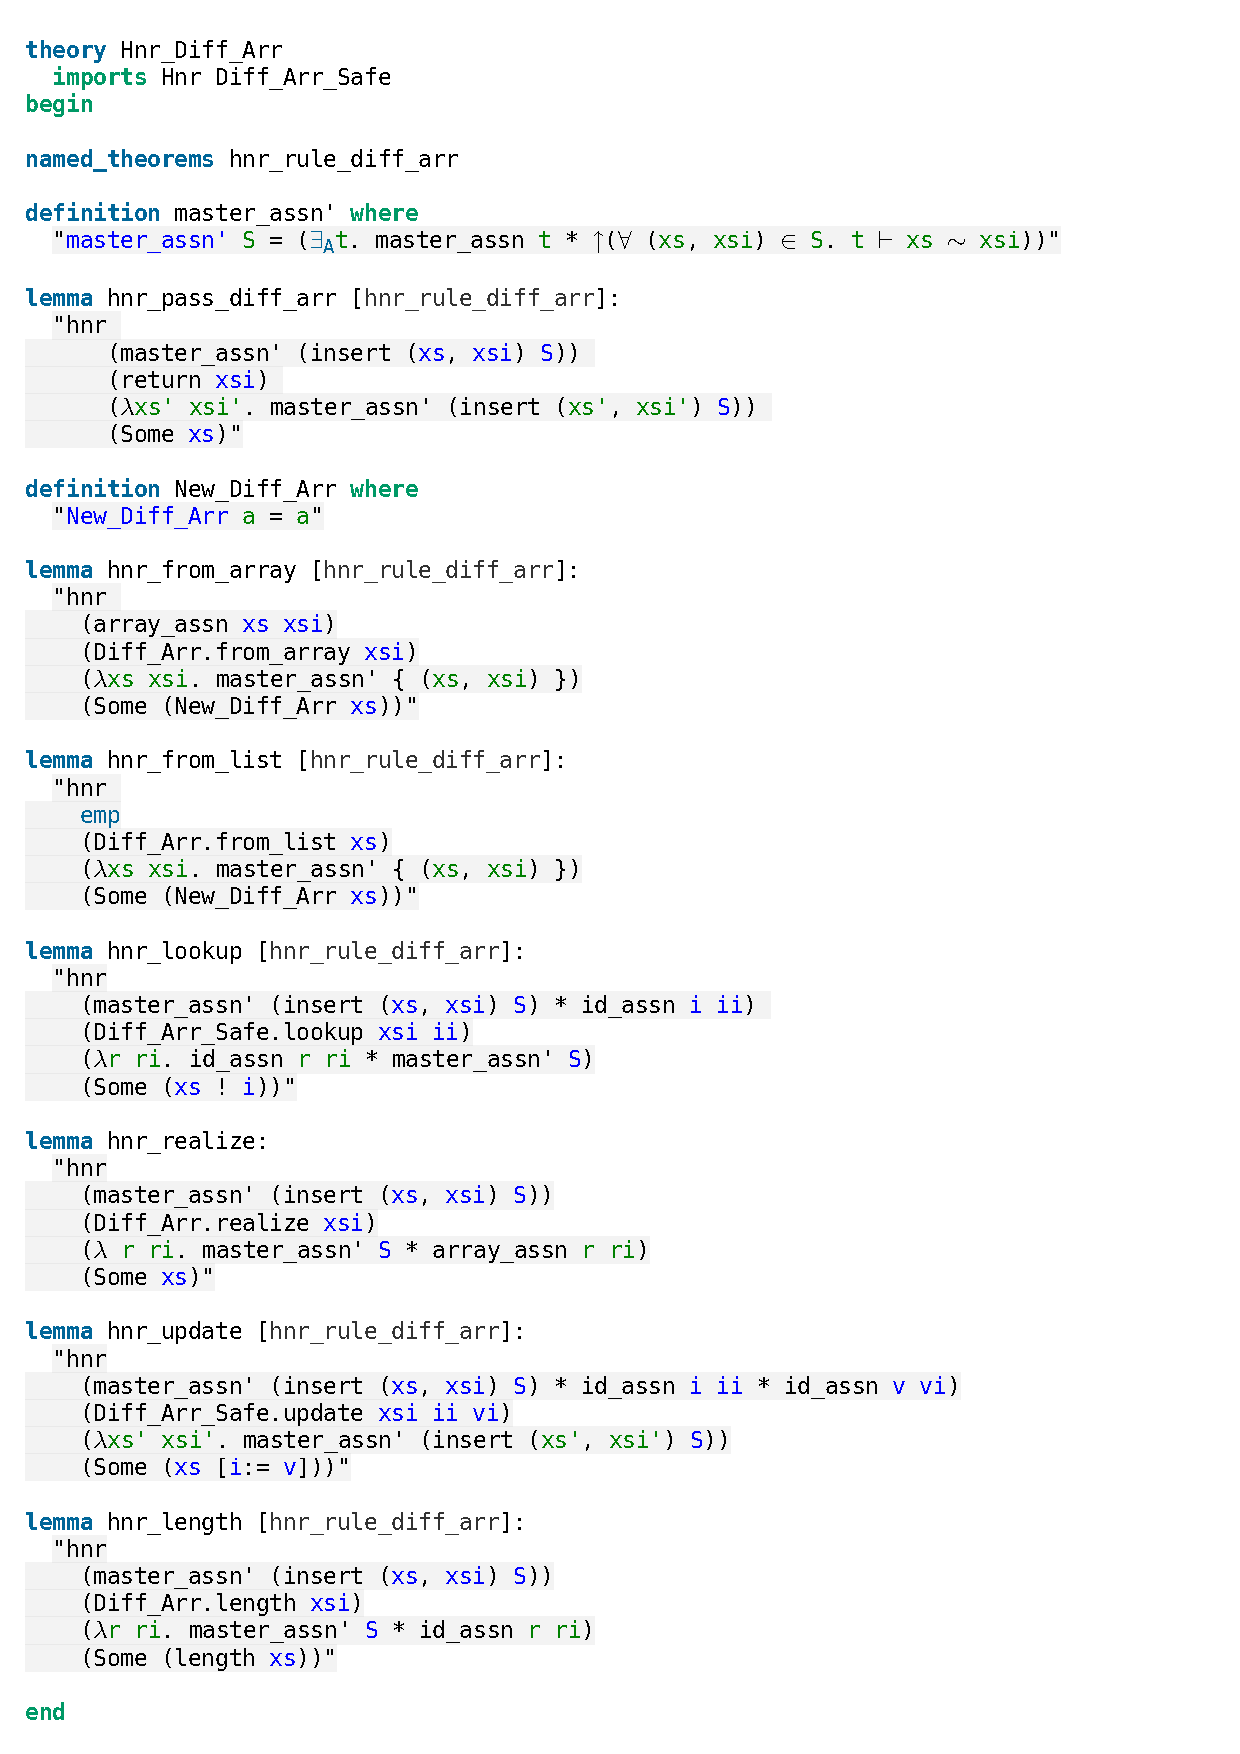
\includegraphics[trim={0 25,4cm 0 3,4cm}, clip, width=1.00\textwidth]{figures/Theory_Hnr_Diff_Arr.pdf}
    \caption[Hnr master assertion]{Hnr master assertion}
    \label{fig:hnr_master_assn}
\end{figure}

\noindent This new version already contains the diff array relation and takes a set of diff arrays and its corresponding list abstractions. These represent all the available versions of the diff array. Further, we ensure again that each variable in each rule has an assertion and collect all the rules in a rule set (\autoref{fig:hnr_diff_arr_rules}). Also, we introduce a definition with the name |New|\_|Diff|\_|Arr| to mark places where a diff array should be created.

\begin{figure}[htpb]
    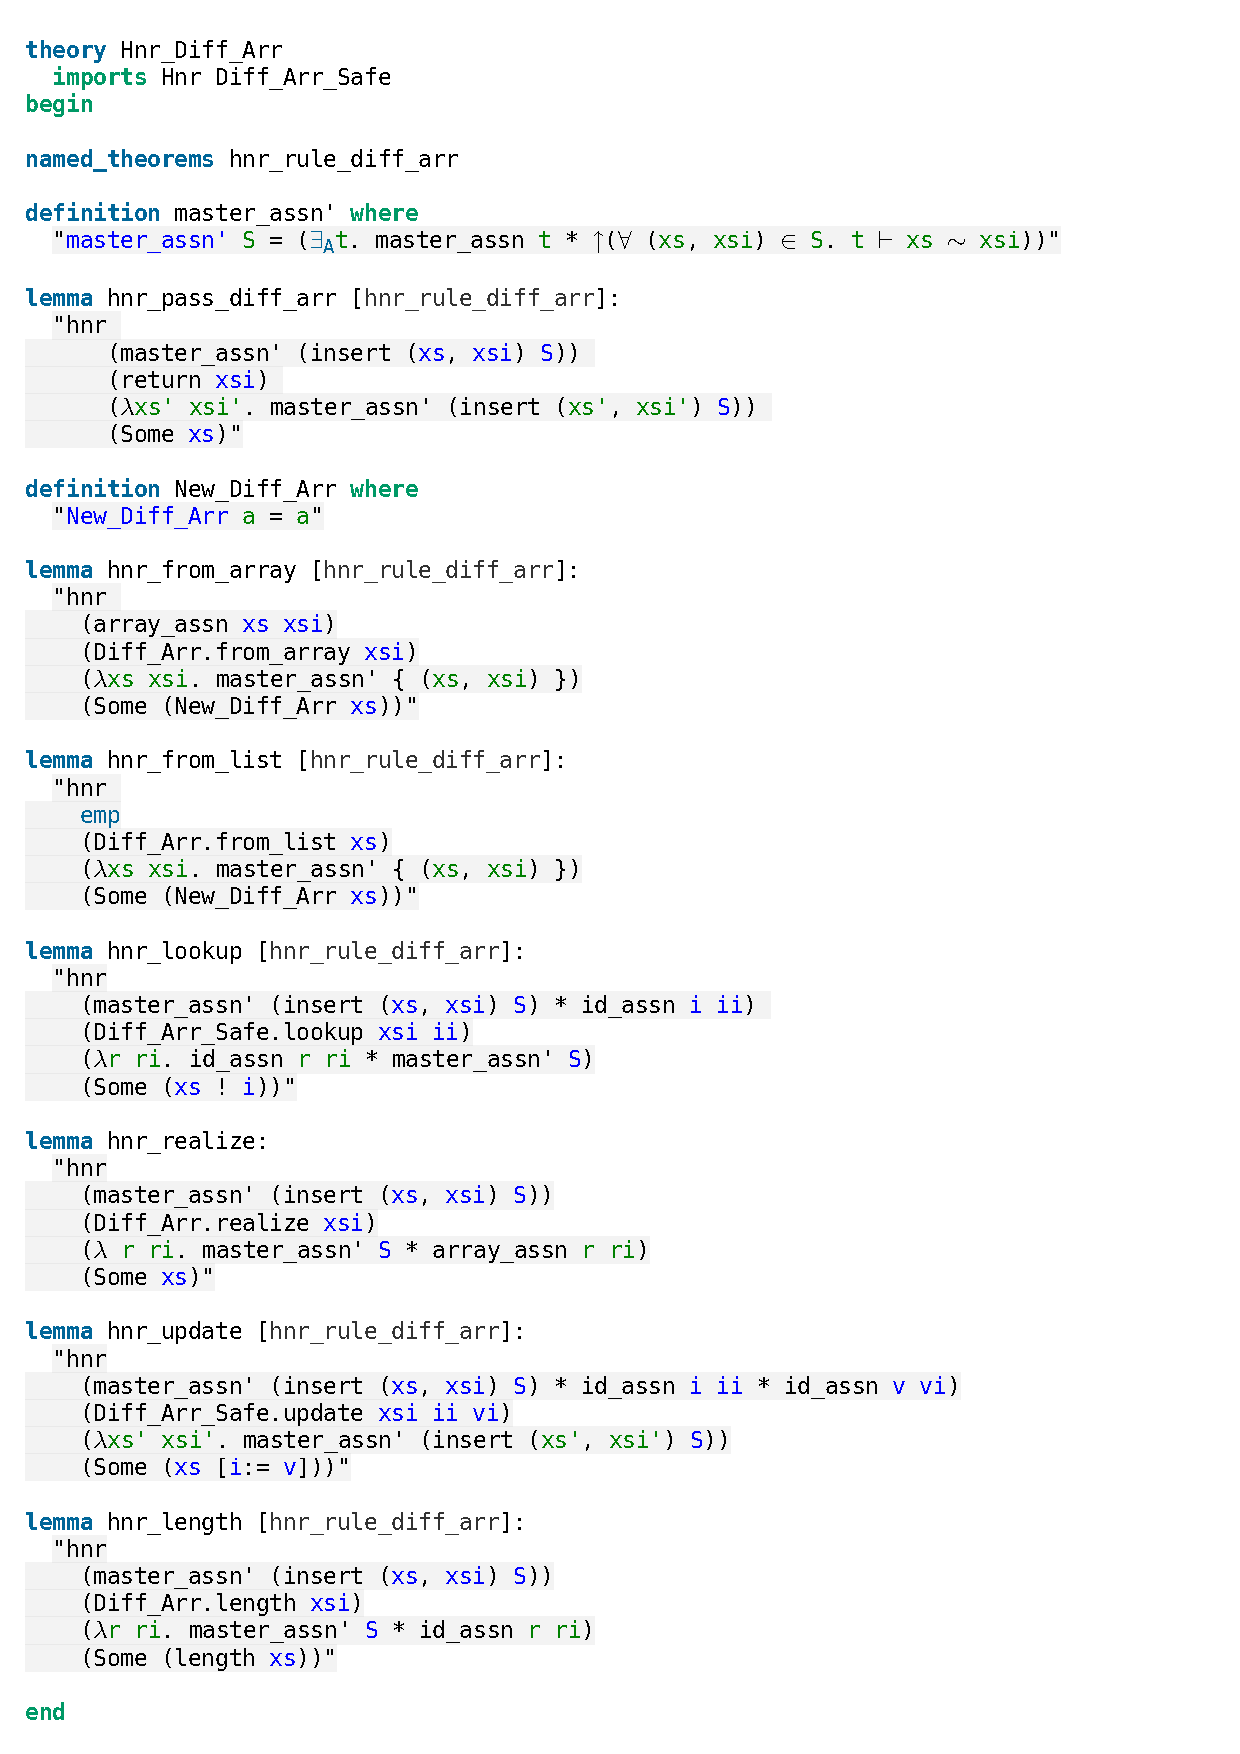
\includegraphics[trim={0 1,2cm 0 4,8cm}, clip, width=1.00\textwidth]{figures/Theory_Hnr_Diff_Arr.pdf}
    \caption[Hnr diff array rules]{Hnr diff array rules}
    \label{fig:hnr_diff_arr_rules}
\end{figure}

\noindent The proofs are again done by converting the |hnr| statements to Hoare triples and then using separation logic proof automation, which relies on the Hoare triple rules from \autoref{section:diff_arr_operations}.

\subsection{Set Inference}

This time we cannot just use reflexivity as the strategy for matching assertions in the frame and for the keep drop method. Simple reflexivity cannot solve goals for inserting elements into the set of the master assertion because the insert operations can be in different orders. We build up a procedure for this case, which we call \textit{set inference} and pass it as the matching strategy to our previously implemented frame inference. The set inference works on rules of the form: |master|\_|assn|' |S| $\Longrightarrow_A$ |master|\_|assn|' |S|'.\\
An example for |S| could be |{a, b, c}| and for |S|' |insert b ?F|. Then, we need to determine if all the elements we know in |S|', and therefore do not belong to the frame, are in |S|. For that, we use a similar approach as for the frame inference previously. \\
As the first step of the set inference, we notice that for solving a goal of the described form, it is enough to solve a goal of the form |S = S|' by applying the rule [].

